\documentclass[a4paper, 12pt, twoside]{book}
	\PassOptionsToPackage{table}{xcolor}
	\usepackage[export]{adjustbox}
	\usepackage[english,ngerman]{babel}
	\usepackage{amsmath, url}
	\usepackage[utf8]{inputenc}
	\usepackage[T1]{fontenc}
	\usepackage{import}
	\usepackage{graphicx}
	\usepackage{subcaption}
	\usepackage{verbatim}
	\usepackage{float}
	\usepackage[headheight=12pt]{geometry}
	\usepackage{fancyhdr}
	\usepackage{subfiles}
	\usepackage{float}
	\usepackage[table,xcdraw,dvipsnames]{xcolor}
  \usepackage{amsmath}
	\usepackage{wrapfig}
\usepackage[rightcaption]{sidecap}
\usepackage[font=small,labelfont=bf,tableposition=top]{caption}
	%  Bibliographie
	\usepackage{bibgerm} % Umlaute in BibTeX
%\usepackage[style=authortitle-icomp]{biblatex}
\bibliographystyle{ieeetr} 
\usepackage[babel,german=guillemets]{csquotes}

	

	\pagestyle{fancy}
	\fancyhf{}
	\fancyhead[LE,RO]{Baran Avinc}
	\fancyhead[RE,LO]{Masterarbeit}
	\fancyfoot[LE,RO]{\vspace{0.05cm}\thepage}
	%\fancyfoot[RE,LO]{\vspace{0.05cm}
\includegraphics[width=0.1\textwidth]{Bilder/TU-Berlin-Logo.pdf}}
	\renewcommand{\headrulewidth}{1pt}
	\renewcommand{\headrule}{\hbox to\headwidth{\color{RoyalPurple}\leaders\hrule height 				\headrulewidth\hfill}}
	\renewcommand{\footrulewidth}{1pt}
	\renewcommand{\footrule}{\hbox to\headwidth{\color{RoyalPurple}\leaders\hrule height \footrulewidth\hfill}}
	\pagestyle{fancy}


	


  	%
\includegraphics[width=0.1\textwidth]{Bilder/TU-Berlin-Logo.pdf}

	





\begin{document}
	
\begin{titlepage}
		\pagestyle{fancy}
		\centering\textbf{\large Masterarbeit zum Thema}\\
		\vspace{3cm} 
		\noindent{\color{RoyalPurple}\rule{\textwidth}{1pt}} \\
		\vspace{0.5cm} 
		\centering\textbf{\large Untersuchung der optischen Polarisation und internen Quanteneffizienz von AlGaN Quantenfilmen mittels temperatur- und leistungsabhängiger Photolumineszenzspektroskopie} \\
		\vspace{0.25cm} 
		\noindent{\color{RoyalPurple}\rule{\textwidth}{1pt}} \\
		\vspace{3cm}
		\centering Baran Avinc \\
		\vspace{3cm}
		\centering Institut für Festkörperphysik
		\vspace{\fill} \\
		\raggedleft{
\includegraphics[width=0.2\textwidth]{Bilder/TU-Berlin-Logo.pdf}}
\end{titlepage}



	\tableofcontents\thispagestyle{fancy}
	
\chapter{Einleitung}
\thispagestyle{fancy}

\begin{quote}
In the spirit of Alfred Nobel the Prize rewards an invention of greatest benefit to mankind; using blue LEDs, white Light can be created in a new way.\end{quote}
Dieser Satz den die Schwedische Akademie der Künste nach der Vergabe des Nobelpreises an die Entwicklung der blauen LED(kurz, light emitting diode) im Jahr 2014 an die Presse veröffentlichte, fasst treffend zusammen, wie hoch die Bedeutung der auf Halbleiterkristallen basierenden optischen Bauelemente ist.
LEDs nehmen einen fundamentalen und immer bedeutender werdenden Teil unseres alltäglichen Lebens ein. Ausgezeichnet durch ihre hervorragende Effizienz, konkurrenzlosen Lebensdauer und geringen Dimension übernimmt sie durch eine immer höher werdenden Lichtausbeute zusehends neue Anwendungsbereiche. 
%Seit jeher etabliert in den Bereichen der optischen Datenübertragung und Leuchtanzeige schreiten immer mehr andere Wellenlängenbereiche in den Fokus der weltweiten Forschung. 
Insbesondere auf Gallium Nitrid (GaN) basierende Halbleitermaterialien haben einen bahnbrechenden Weg hingelegt, der zur Entwicklung von hoch effizienten und leuchtstarken blauen LEDs führte.



	\chapter{Grundlagen}
\thispagestyle{fancy}

\section{Bandstruktur von Gruppe-III Nitriden}
\begin{figure}[!htb]
    \centering
    \begin{minipage}[t]{\linewidth}
        \centering
        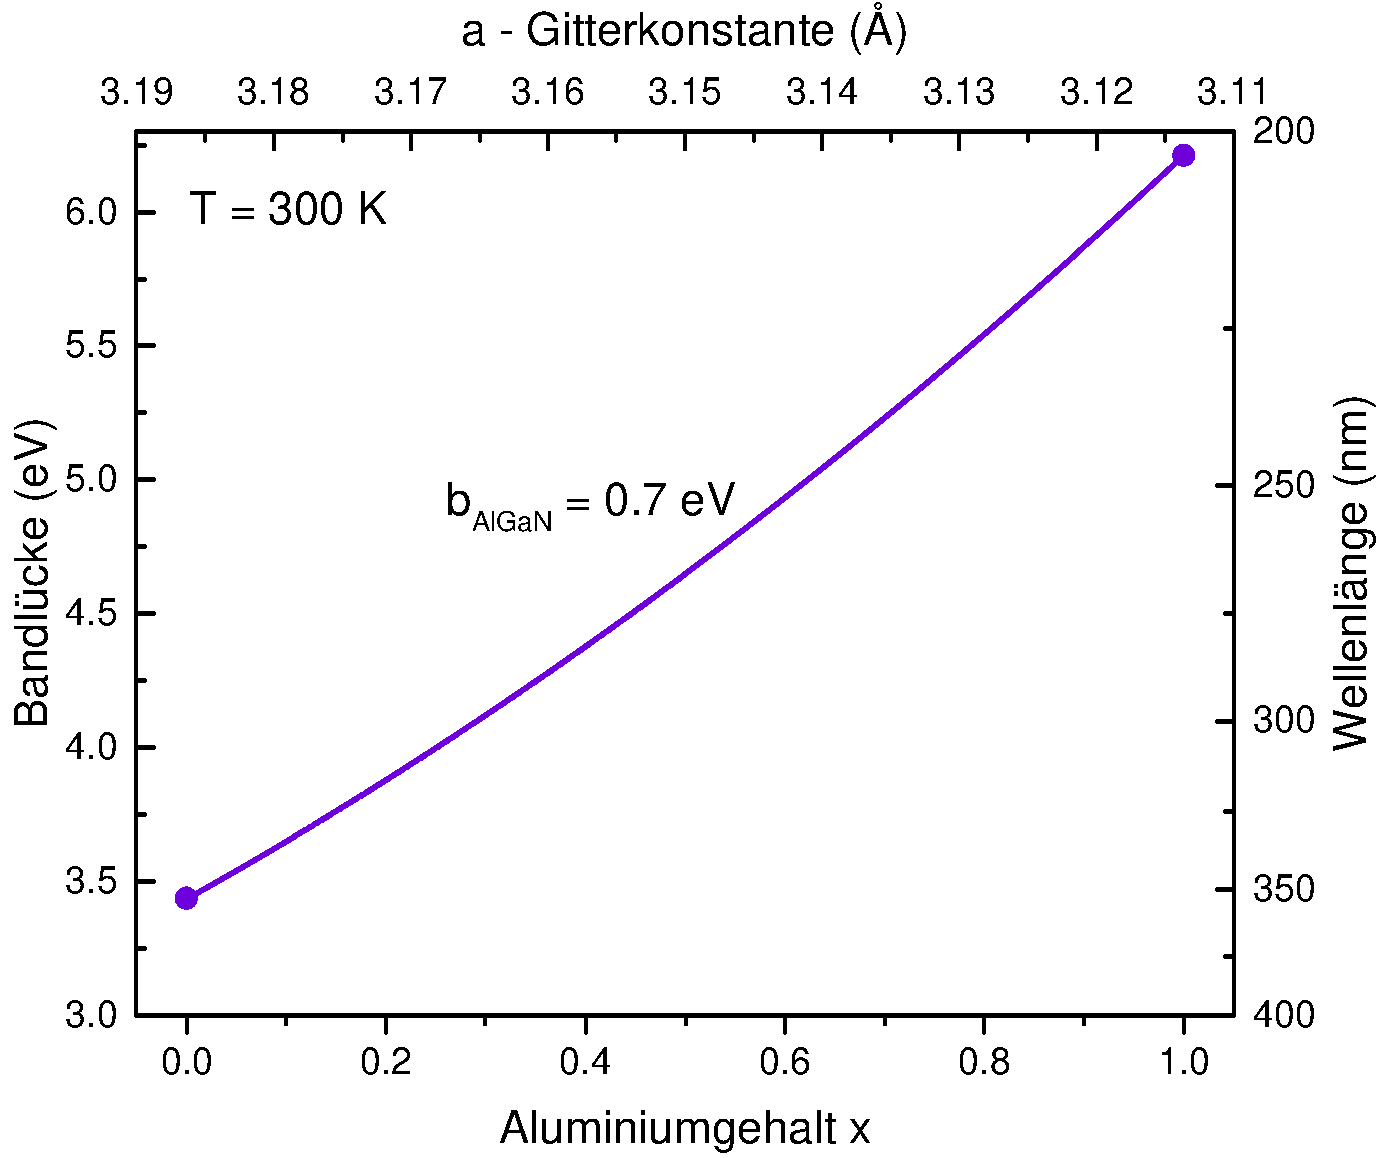
\includegraphics[width=0.5\linewidth]{Bilder/bandluecke.pdf}
        \caption{Die Bandlücke von $Al_{x}Ga_{1-x}N$ variiert mit dem Aluminiumgehalt x zwischen den Bandlücken von AlN ($E_{g}(T = 300 K) = 6,213 \thinspace eV$) und GaN ($E_{g}(T = 300 K) = 3,437 \thinspace  eV$) ~\cite{pipr}. Die Abweichung von der Linearität beschreibt der Bowing-Parameter $b_{AlGaN} = 0,7 \thinspace eV$.} 
        \label{fig:wurtz}
    \end{minipage}% <- sonst wird hier ein Leerzeichen eingefügt
\end{figure}
\noindent
Der Schwerpunkt dieser Arbeit liegt auf dem AlGaN-Materialsystem mit hohen Al-Konzentrationen. Das Mischverhältnis bestimmt hierbei die Bandlückenenergie des Verbindungshalbleiters. Durch die unterschiedlichen Bandlückenenergien von Aluminium mit $6,03 \thinspace eV$\cite{fenaln} und GaN mit $3,4 \thinspace eV$ \cite{pipr} eignet sich AlGaN besonders für die Emission im Wellenlängenbereich von UV-A bis UV-C. 
Die Bandlückenenergie von AlGaN lässt sich durch Interpolation der binären Energien von GaN und AlN in Abhängigkeit des Kompositionsverhältnisses x berechnen, wobei ein zusätzlicher Bowing-Parameter für die nichtlineare Abweichung hinzugefügt wird. 
%
\begin{equation}
    E_{Al_{x}Ga{1-x}N} = E_{AlN} \cdot x + E_{GaN} \cdot (1-x) - b_{AlGaN} \cdot x \cdot (1-x) 
\end{equation}
%
Die Gruppe um Lee et al. gibt nach Auswertung der in der Literatur vorkommenden unterschiedlichen Bowing-Parameter für $Al_{x}Ga_{1-x}N$ einen Wert von $b_{AlGaN} = 0,62\thinspace(\pm \thinspace 0,45)\thinspace eV$ an und ergänzt, dass hohe Wachstumstemperaturen zu großen Bowing-Parametern führen \cite{doi:10.1063/1.123339}.
Vurgaftman et al. empfehlen unter Berücksichtigung weiterer Veröffentlichungen für $b_{AlGaN} =  0,7 \thinspace eV$.



\section{Wurtzitstruktur}

\begin{figure}[!htb]
    \centering
    \begin{minipage}[t]{\linewidth}
        \centering
        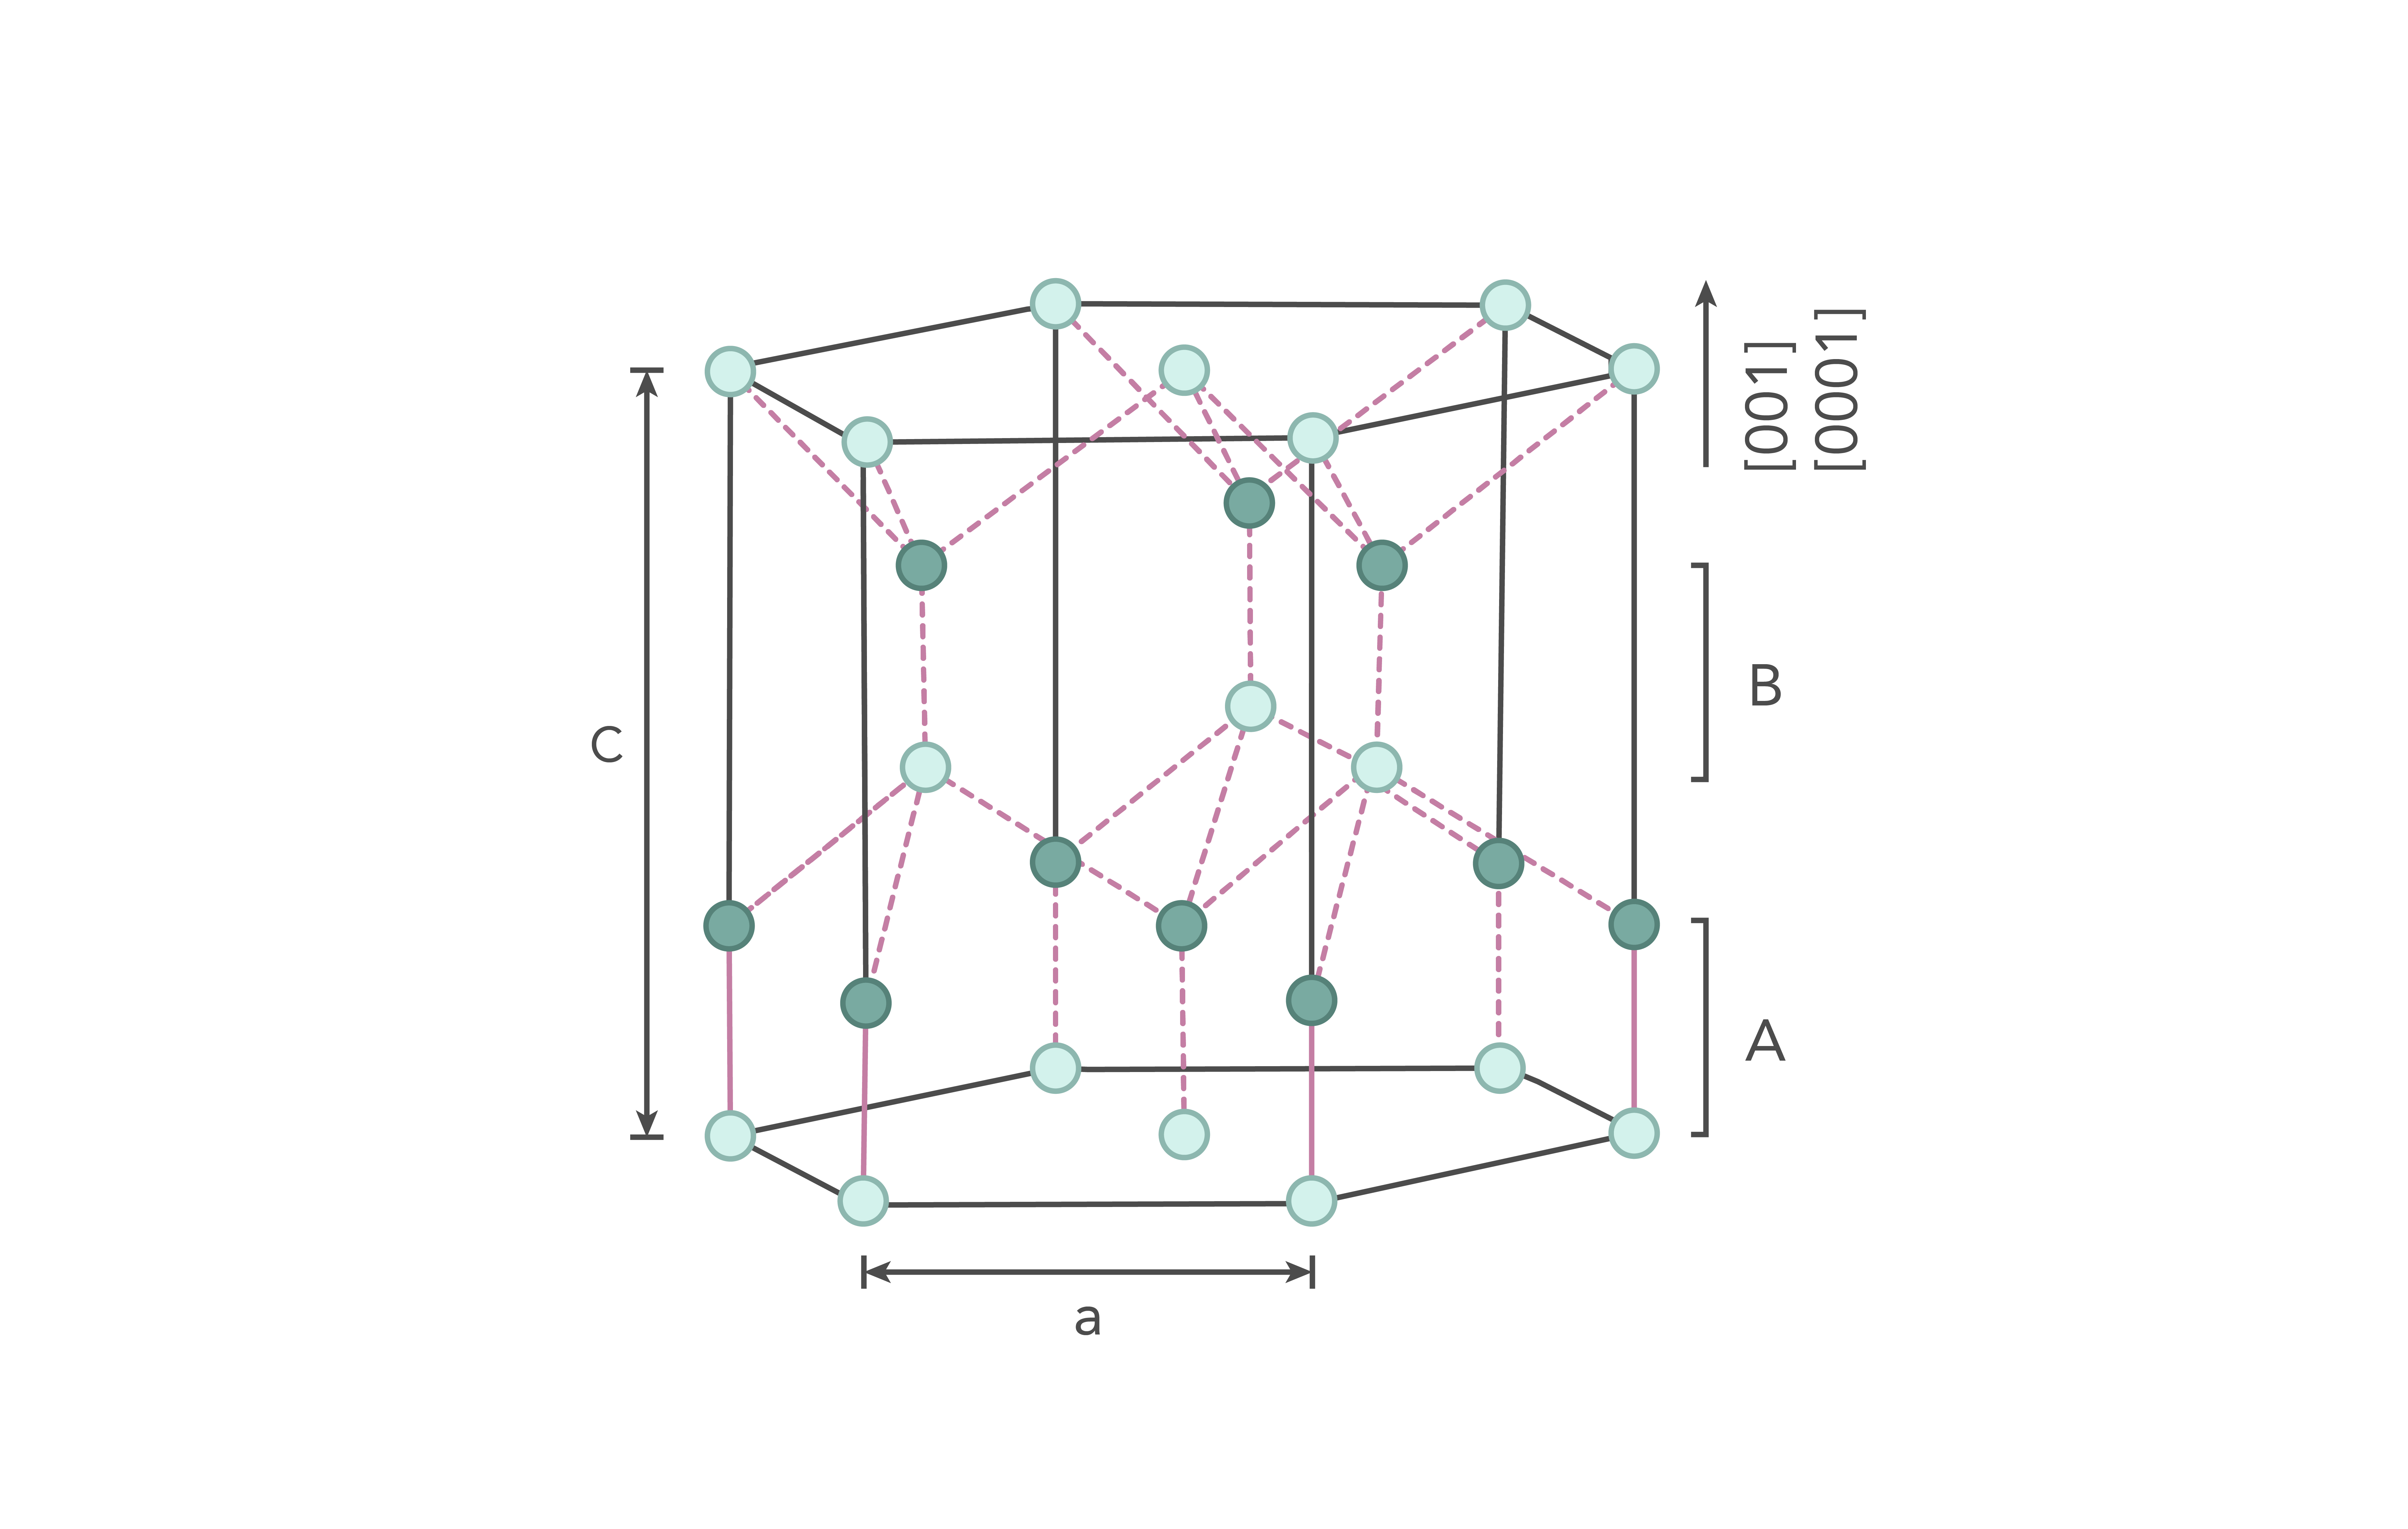
\includegraphics[width=0.8\linewidth]{Bilder/Wurtzite.png}
    \end{minipage}% <- sonst wird hier ein Leerzeichen eingefügt
     \caption{Einheitzelle der hexagonalen Wurtzitstruktur. Die schwarzen Kreise stellen die Position der Stickstoffatome im Gitter dar. Die Gitterposition der Gruppe-III-Metallatome sind als graue Kreise dargestellt. A und B bezeichnen die Stapelebenen.}
        \label{fig:wurtz}
\end{figure}
\noindent
Die wichtige Gruppe der III-Nitridhalbleiter setzt sich aus den Metallen
der dritten Hauptgruppe Aluminium (Al), Gallium (Ga) und Indium (In) zusammen.
Diese kristallisieren, wie in Abbildung \ref{fig:wurtz} zu sehen, bevorzugt in der hexagonalen Wurtzitstruktur. Anschaulich bedeutet dies, dass ausgehend von der hexagonal dichtesten Kugelpackung in Doppellagen, die Gruppe-III-Metalle und Stickstoff (N) sich entlang der c-Achse in der Abfolge A-B-A-B anordnen \cite{buchc}. Die Einheitszelle wird durch Gitterparameter $a$ und $c$ bestimmt. Die Gitterkonstanten zeigen eine lineare Abhängigkeit vom Konzentrationsverhältnis x und können mit dem Vegard'schen Gesetz berechnet werden.
%
\begin{align}
\begin{split}
    a_{Al_{x}Ga{1-x}N} &= a_{AlN} \cdot x + A_{GaN} \cdot (1-x)  ,
    \\
    c_{Al_{x}Ga{1-x}N} &= c_{AlN} \cdot x + A_{GaN} \cdot (1-x) 
\end{split}
\end{align}
%
Die Tabelle \ref{table:tab1} zeigt die typischen Gitterkonstanten.
\begin{figure}[H]
\centering
\begin{tabular}{|c|c|c|c|}
\hline
\multicolumn{1}{|l|}{Gitterkonstante} & AlN & GaN & Saphir \\ \hline \hline
a & 3,112 & 3,192 & 4,758 \\ \hline
c & 4,980 & 5,196 & 12,99 \\ \hline
\end{tabular}
\caption{Übersicht der Gitterkonstanten der binären Halbleiter AlN, GaN und $Al_{2}O_{3}$ (Saphir). ~\cite{pohl} }
\label{table:tab1}
\end{figure}

\section{Polarisationsfeld und QCSE in III/V Halbleitern}

Aufgrund der fehlenden Inversionssymmetrie und stark unterschiedlichen Elektronegativitäten des Stickstoffs und der entsprechenden Gruppe III-Metalle bilden sich Polarisationsfelder aus, die entlang der auf der Basalebende stehenden c-Achse verlaufen. Hier unterscheidet man zwischen zwei Arten von Polarisationsfeldern, die spontane Polarisation $ \vec{P}^{sp} $ und die piezoelektrische Polarisation $ \vec{P}^{pz} $. Die spontane Polarisation entsteht durch Dipolmomente im Kristall, die sich aufgrund von ungleichen Bindungslängen nicht komplett aufheben. Ursprung der 
Dipolmomente im AlGaN sind die unterschiedlichen Elektronegativitäten zwischen den Gruppe III-V Elementen. Bedingt durch die angestrebte Minimierung der Gesamtenergie kommt es zur Abweichung vom idealen Tetraederwinkel von $109,5^{\circ}$~\cite{ambacher2002}.
%
\begin{figure}[htb]
    \centering
    \begin{minipage}[t]{1.0\linewidth}
        \centering
        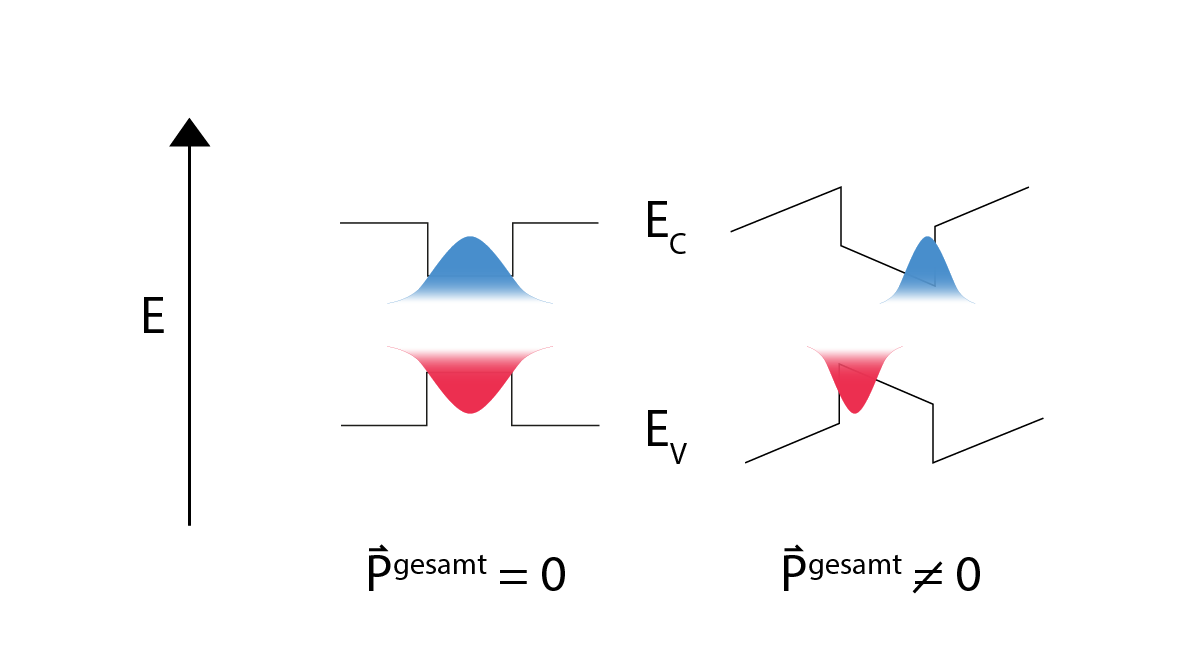
\includegraphics[width=0.7\linewidth]{Bilder/QCSE.png}
    \end{minipage}% <- sonst wird hier ein Leerzeichen eingefügt
    \caption{Einfluss der spontanen und piezolektrischen Polarisation auf Valenz- und Leitungsband einer Quantenfilm-Heterostruktur. Die Aufenthaltswahrscheinlichkeiten von Elektronen und Löchern werden verschoben.}
        \label{fig:qcse}
\end{figure}
\noindent
Die Ursache für die piezoelektrische Polarisation sind die Verspannungen zwischen den in (0001)-Richtung gewachsenen Schichten, welche durch die unterschiedlichen thermischen Ausdehnungskoeffizienten und die Gitterfehlanpassung beim pseudomorphen Wachstum entstehen. Sie wird berechnet nach
%
\begin{equation}
    \vec{P}^{pz} = e \cdot \epsilon
\end{equation}
%
mit Dehnung $\epsilon$ und dem piezolektrischen Tensor $\vec{e}$ (Tensor dritter Stufe).
\newline
In Heterostrukturen führt der Wechsel der Gesamtpolarisation $\vec{P}^{gesamt} = \vec{P}^{pz} + \vec{P}^{sp}$ zwischen den einzelnen Schichten zur Ansammlung von Ladungsträgern an den Grenzflächen. Dies ist insbesondere für die Effizienz von Leucht-und Laserdioden von Nachteil. Denn in diesen erzeugen die induzierten Grenzflächenladungen ein elektrisches Feld, das zur einer Bandverbiegung führt (siehe Abb. \ref{fig:qcse}). Mit dem Einfluss der Polarisation sammeln sich die Elektronen und Löcher im Quantenfilm somit auf gegenüberliegenden Seiten. Dies führt dazu, dass der räumliche Überlapp der Wellenfunktionen von Elektronen und Löchern abnimmt. Durch das verringerte Überlappintegral der Wellenfunktionen sinkt nach Fermis Goldener Regel auch die strahlende Rekombinationsrate. Dieser Effekt wird als "Quantum Confined Stark Effekt"  (QCSE) bezeichnet. Des Weiteren sinkt die effektive Bandlücke und ist im Spektrum durch eine Rotverschiebung der Emission zu erkennen. Bei hohen Ladungsträgerdichten im Quantenfilm kommt es zur Abschirmung (engl. screening) der Grenzflächenladungen, welche die Auswirkungen des Effektes abschwächen.

	%
\thispagestyle{fancy}


\section{Rekombinationsmechanismen}
%
\begin{figure}[h]
\centering
\begin{minipage}[t]{1\linewidth}
\centering
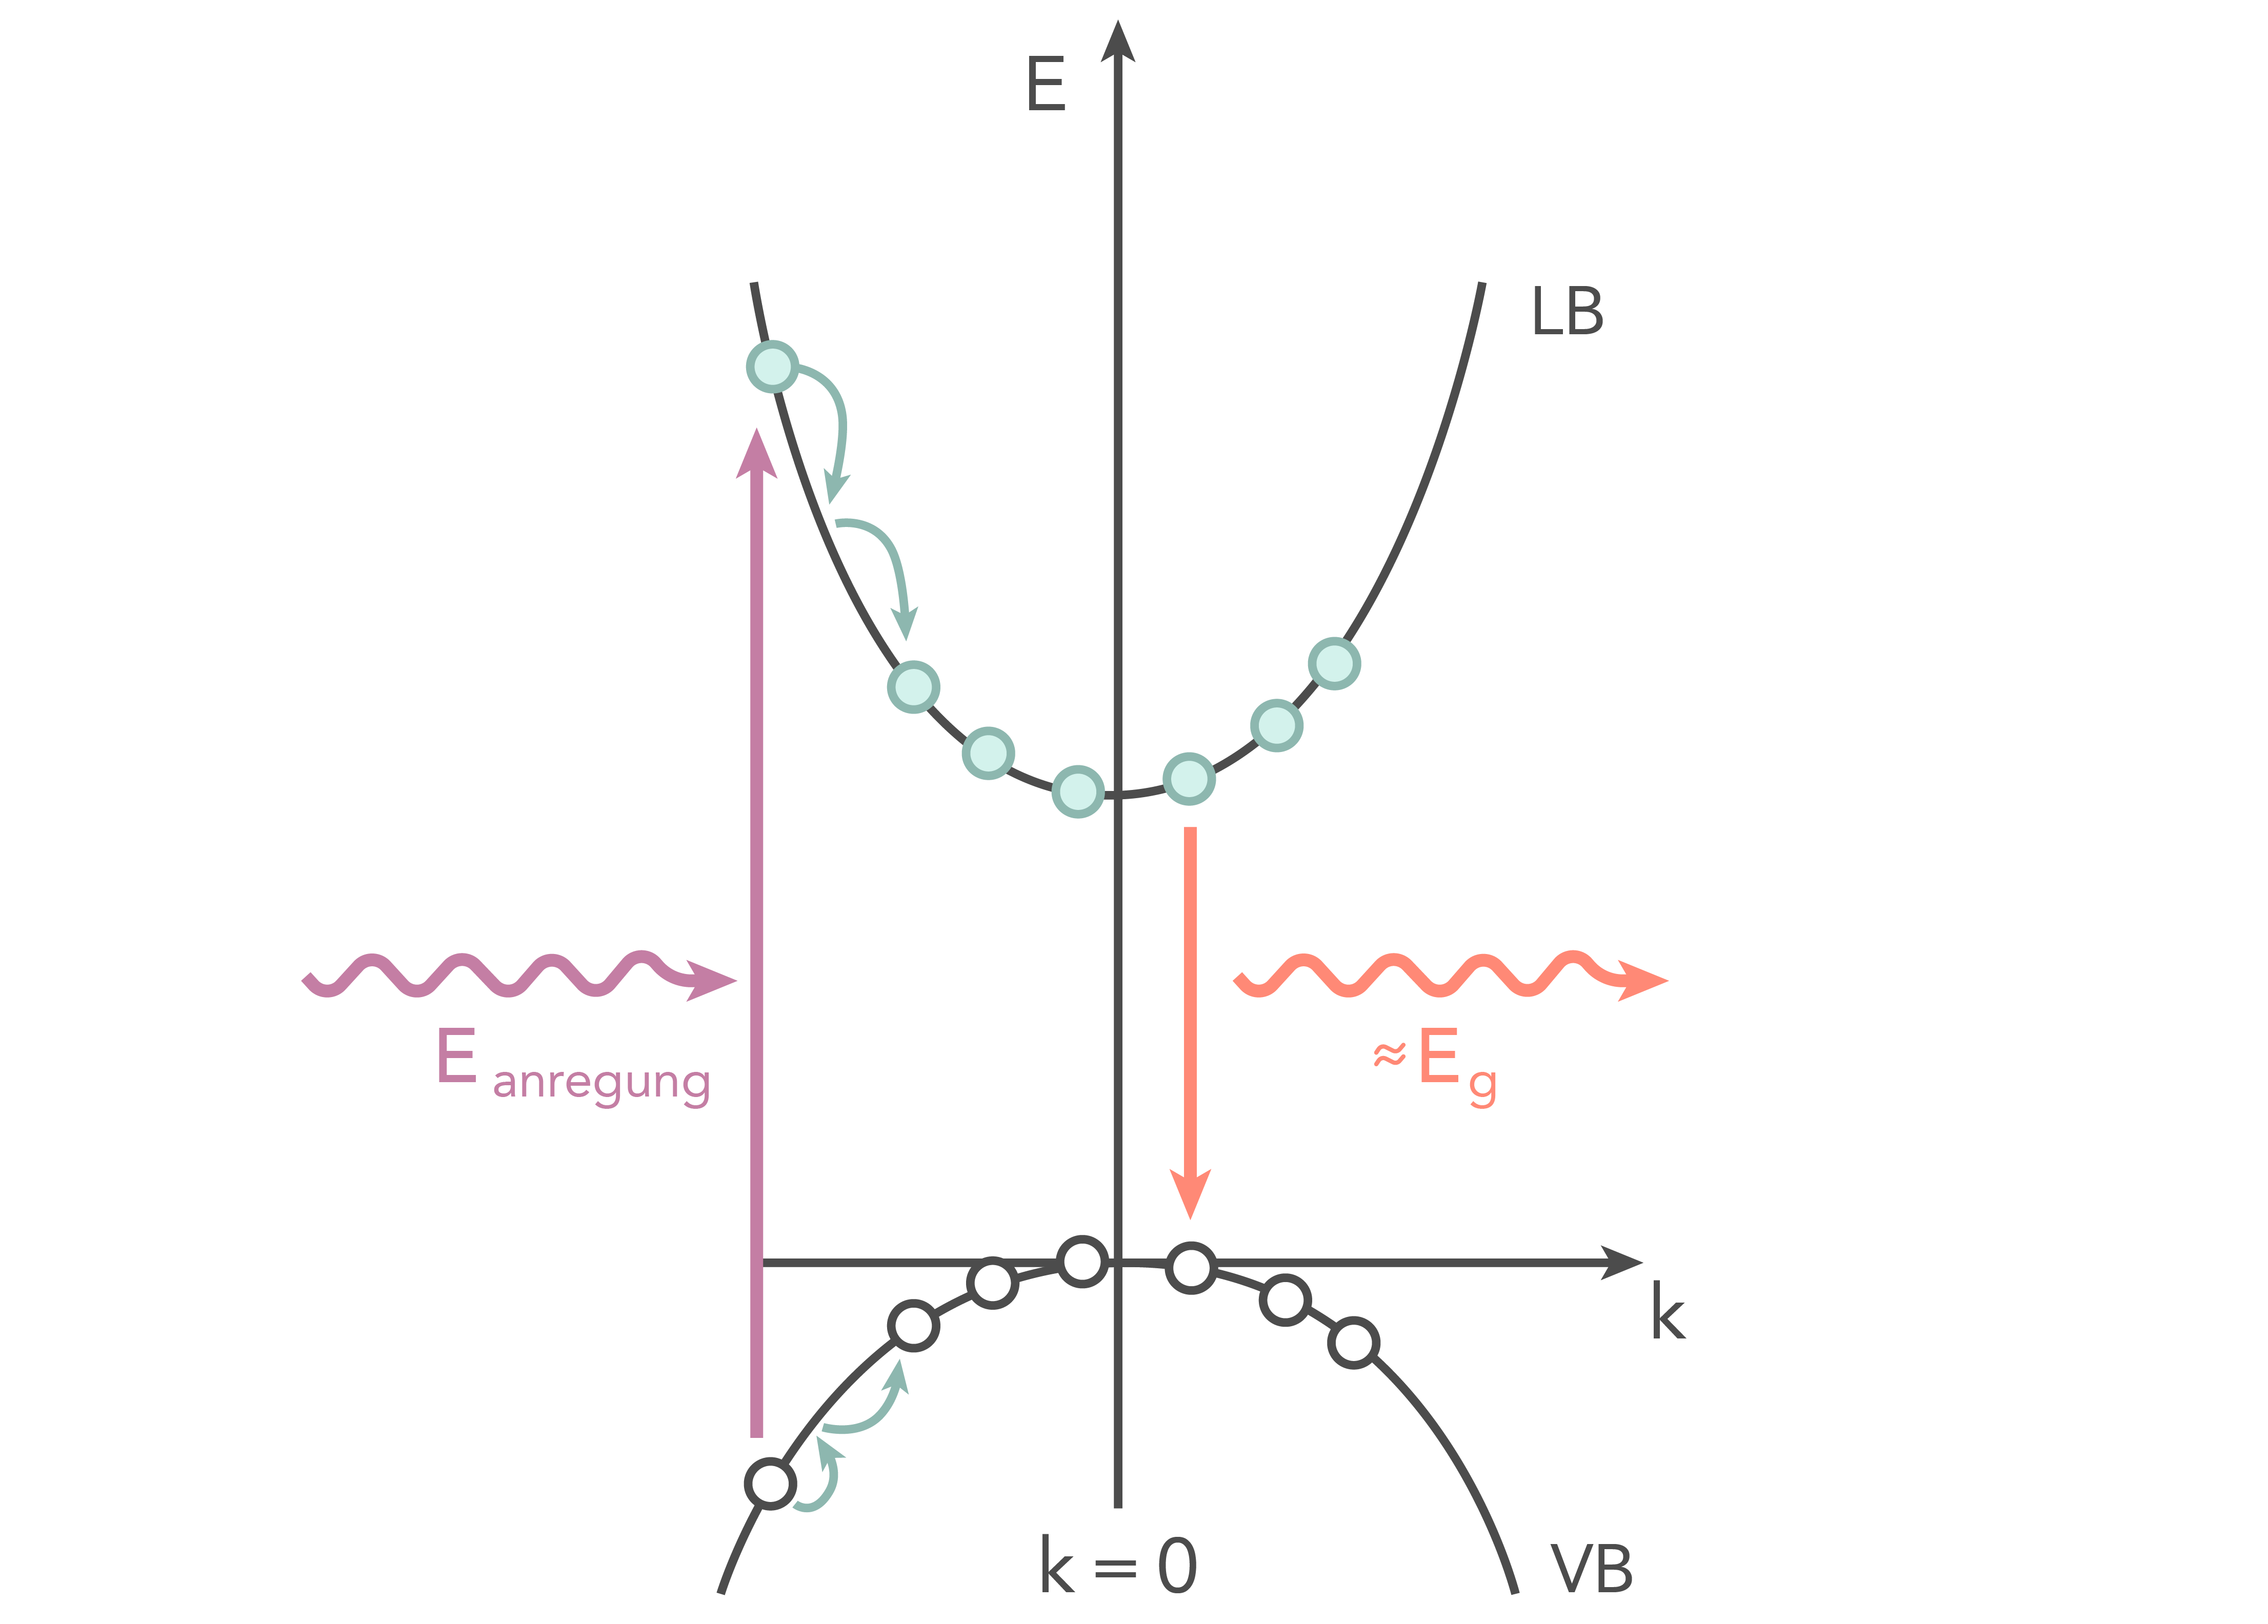
\includegraphics[width=0.8\linewidth]{Bilder/bandrekomb.png}
\end{minipage}% <- sonst wird hier ein Leerzeichen eingefügt
\caption{Durch Einstrahlung eines Photons ausreichender Energie, können Elektronen vom Valenzband in das Leitungsbands angeregt werden. Von dort aus rekombinieren Elektronen und Loch entweder strahlend unter Aussendung eines Photons oder nicht-strahlend.}
 \label{fig:bandrekomb}
\end{figure}
\noindent
In der Photolumineszenzspektroskopie wird Licht als Anregungsquelle von Halbleitermaterialien für die Erzeugung eines Elektron-Loch-Paars benutzt. Dabei wird ein Elektron aus dem Valenzband in das Leitungsband angehoben und ein Loch zurückgelassen wie in Abbildung \ref{fig:bandrekomb} gezeigt wird. Die Elektronen relaxieren anschliessend sehr schnell in das Minimum des Leitungsbandes und analog die Löcher in das Minimum des Valenzbandes Abb. . Leitung-und Valenzband befinden sich im Fall von AlGaN am gleichen $\vec{k}$ Vektor im reziproken Raum, dem sog. $\Gamma$ -Punkt. Das macht das Materialsystem AlGaN zu einem direkten Halbleiter, was von besonderem Vorteil ist. Denn ein direkter Bandübergang, ist die wichtigste Grundlage für eine effiziente halbleiterbasierte Lichtquelle. Denn die Wahrscheinlichkeit einer Anregung und daraufhin folgender Rekombination unter Aussendung eines Photons ist deutlich höher, da kein Phonon am Prozess beteiligt sein muss (Abb. \ref{fig:rekombphoton}). 
\begin{figure}[htb]
    \centering
    \begin{minipage}[t]{0.49\linewidth}
        \centering
        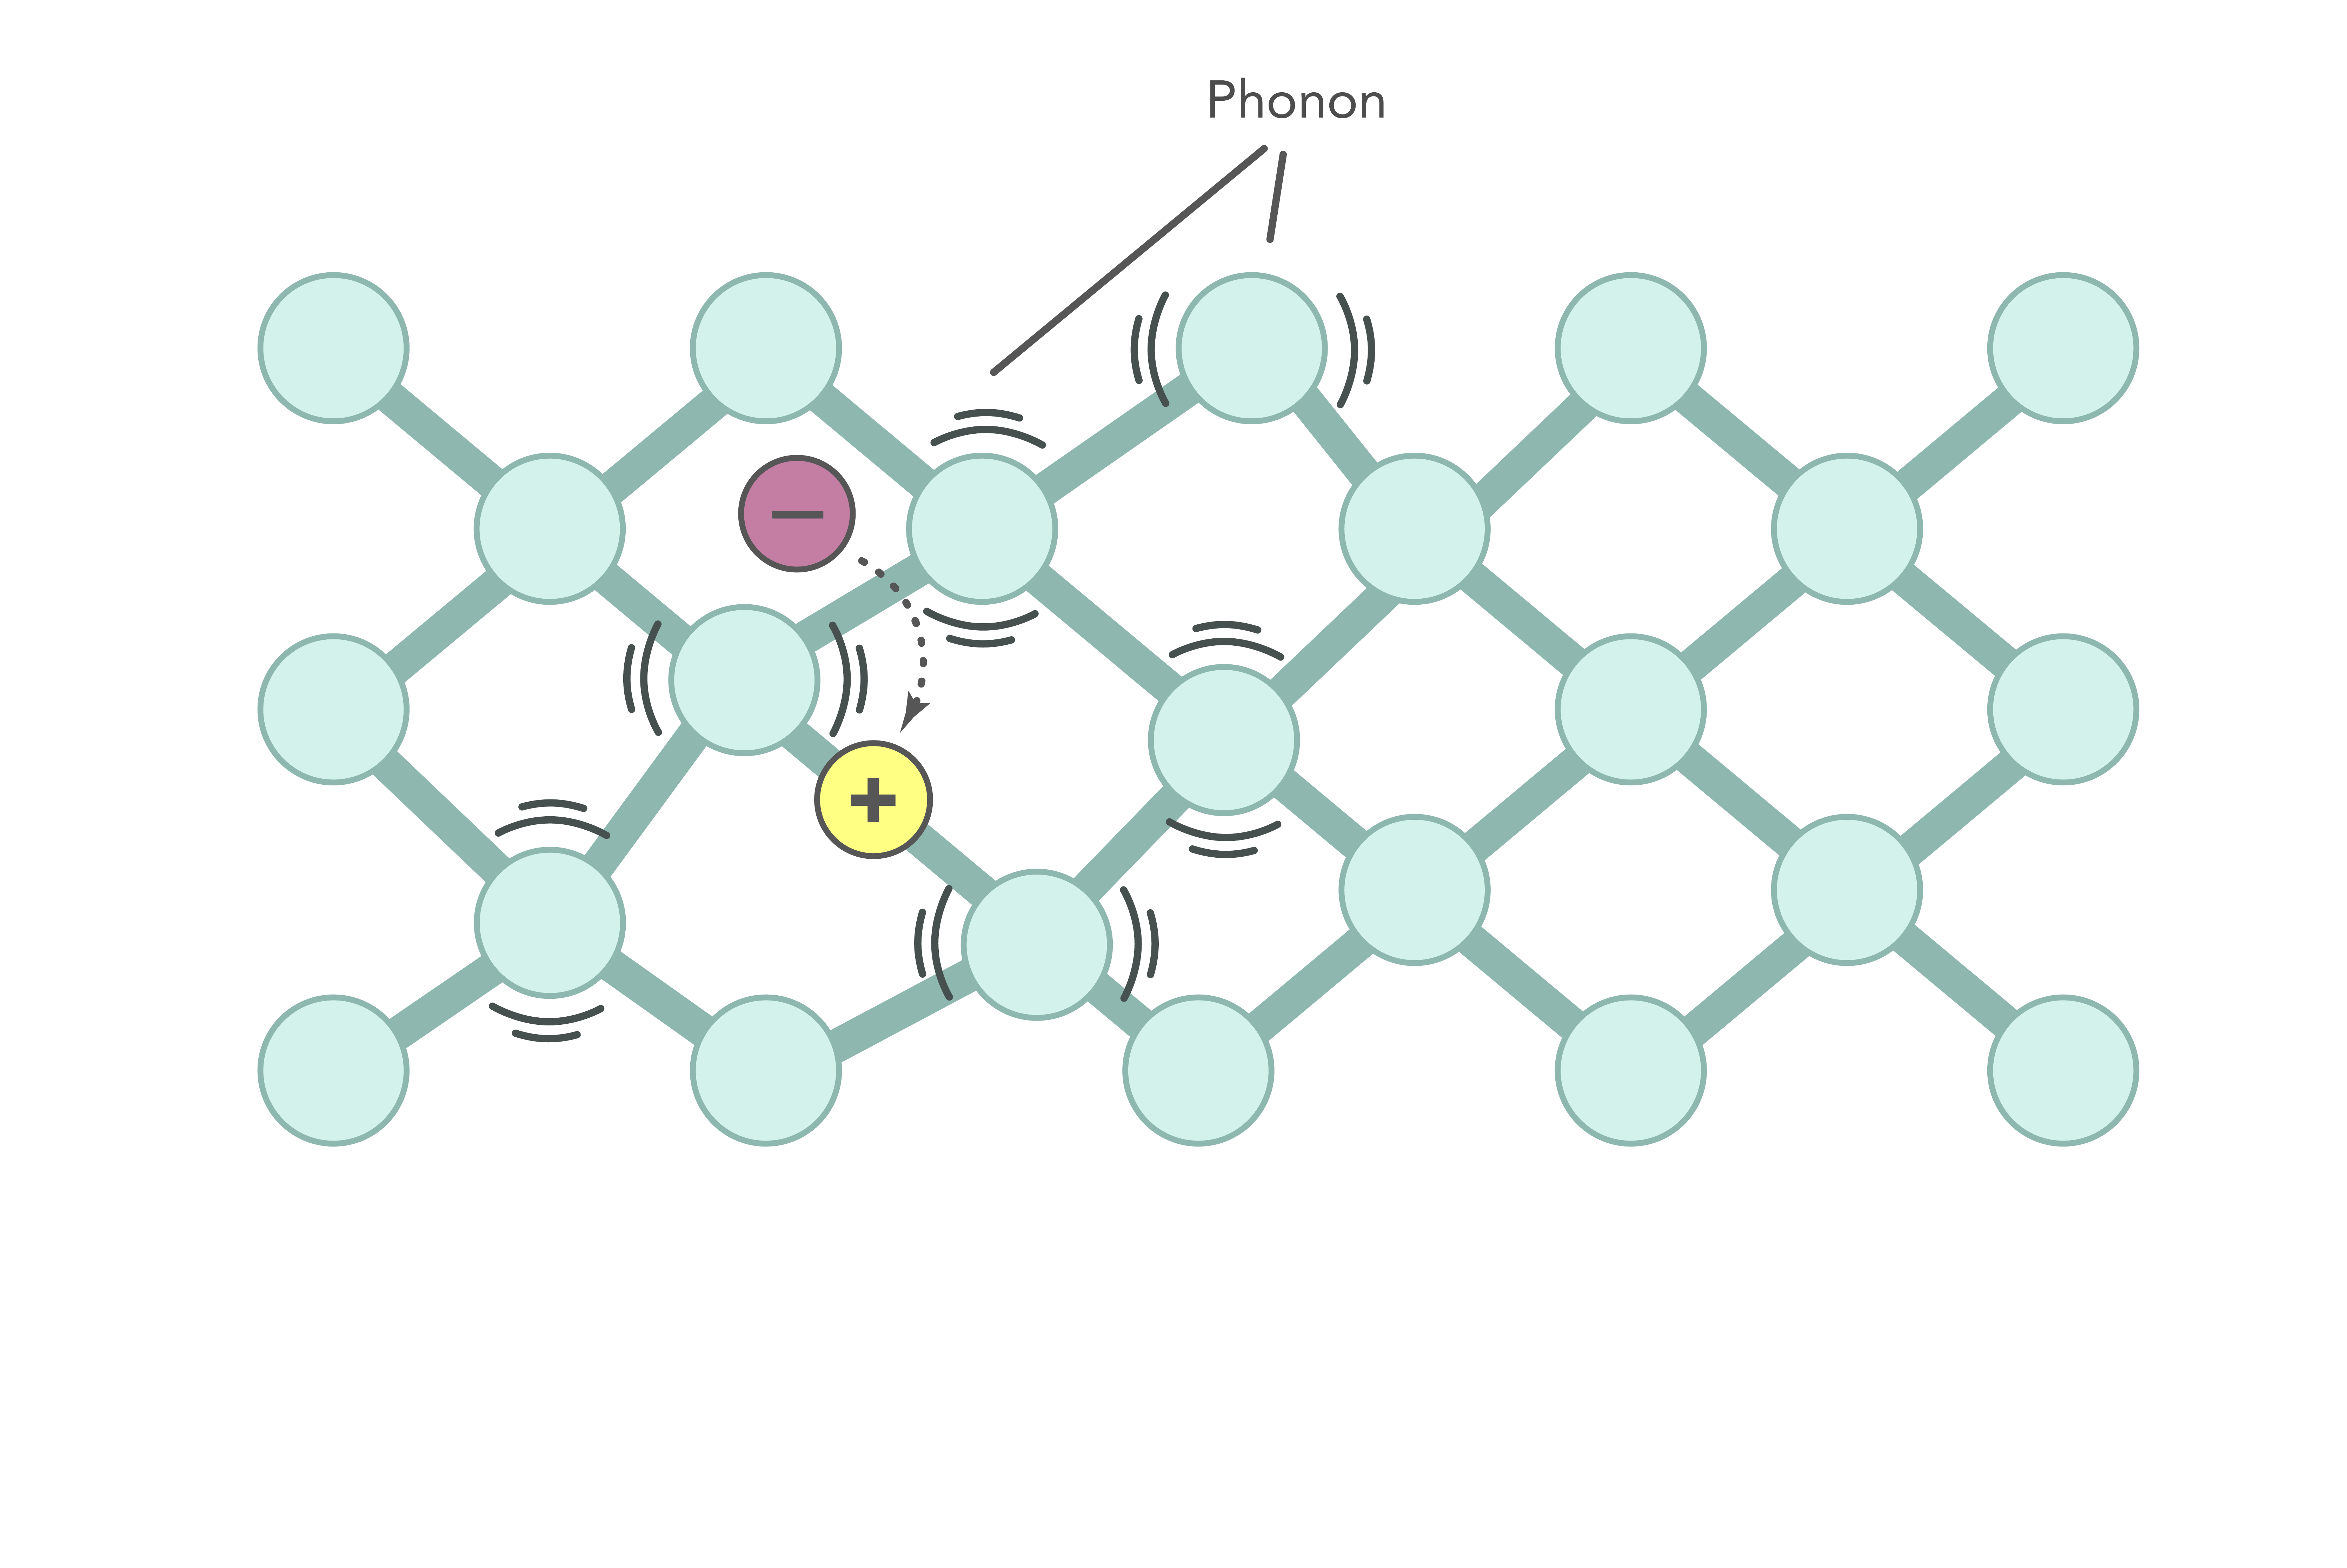
\includegraphics[width=\linewidth]{Bilder/nonradRekomb.png}
        \caption{Rekombination von Elektron und Loch unter Teilnahme eines Phonons.}
    \end{minipage}% <- sonst wird hier ein Leerzeichen eingefügt
    \hfill
    \begin{minipage}[t]{0.49\linewidth}
        \centering
        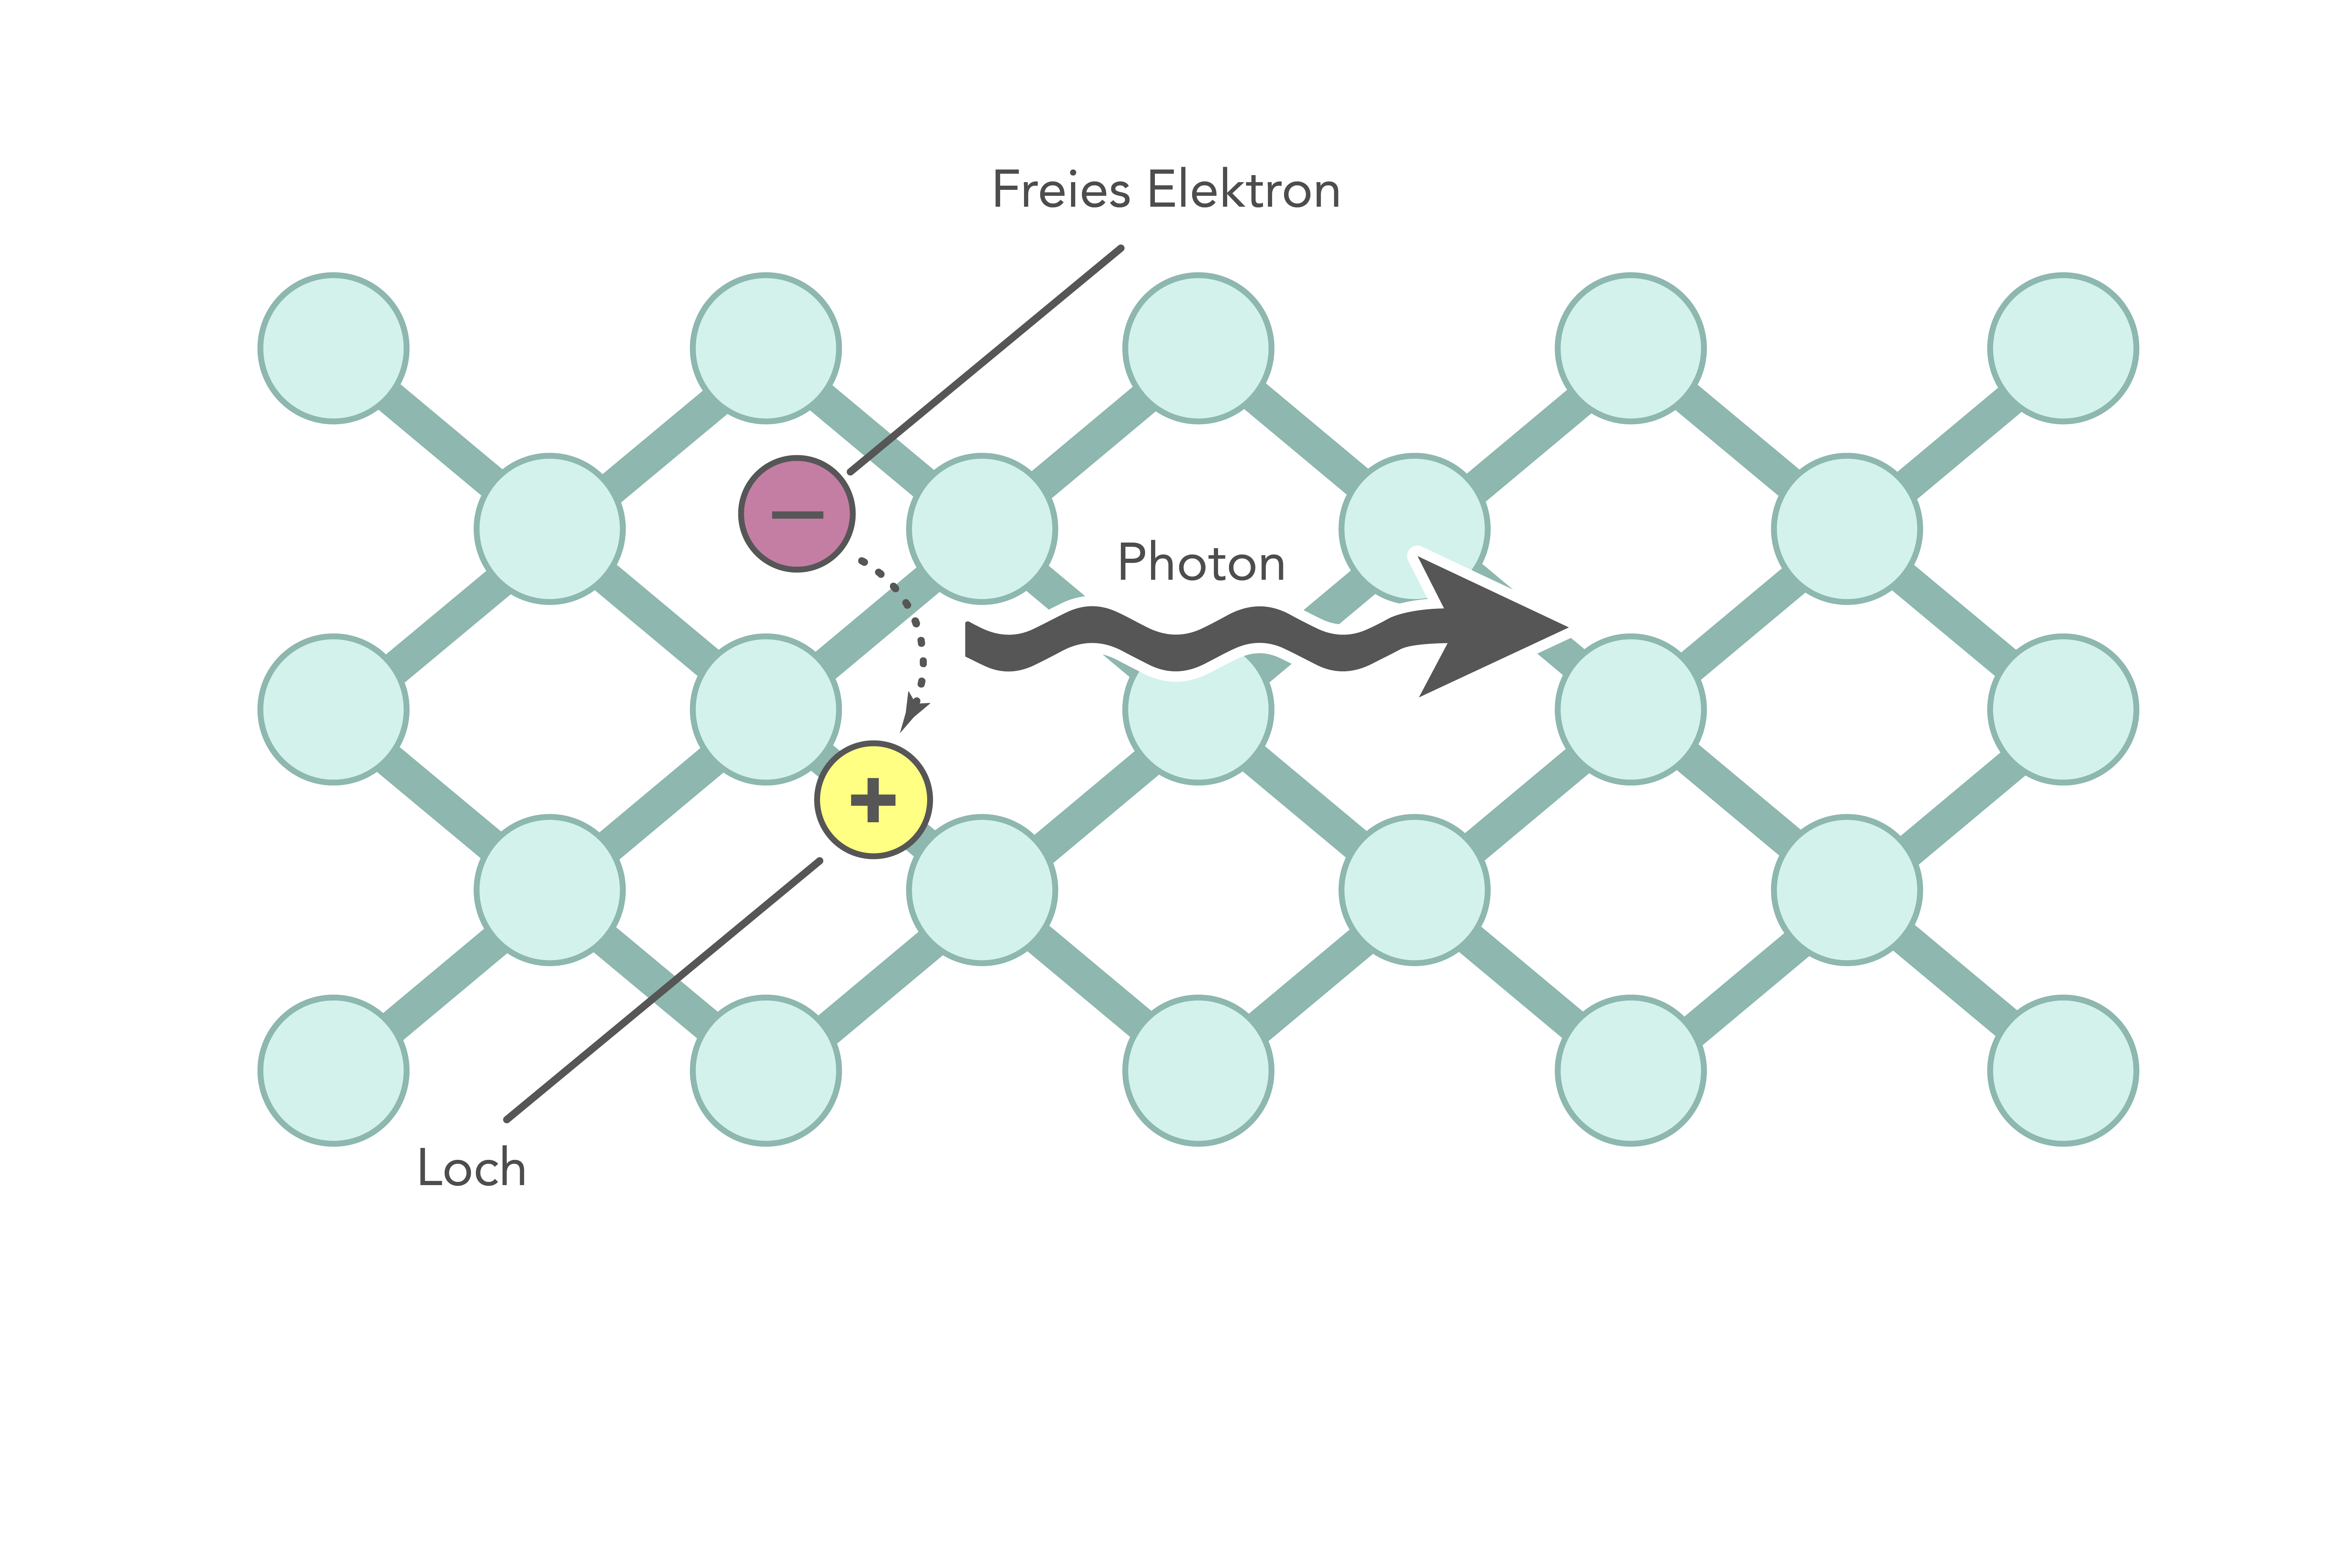
\includegraphics[width=\linewidth]{Bilder/radRekomb.png}
        \caption{Radiative Rekombination von Elektron und Loch und Aussendung eines Photons}
    \end{minipage}
		\label{fig:rekombphoton}
\end{figure}
\noindent
Die Rekombination kann dennoch auch nicht-strahlend erfolgen, weil epitaktisch gewachsene Halbleitersstrukturen herstellungsbedingt beispielsweise nicht ohne ungewollte Dotierung durch Fremdatome, Versetzungen oder Fehlstellen an Atomgitterplätzen (Vakanzen) gewachsen werden können. Diese als sogenannten Störstellen fungieren und diskrete Energieniveaus haben, 
%
\begin{figure}[h]
    \centering
    \begin{minipage}[t]{0.75\linewidth}
        \centering
        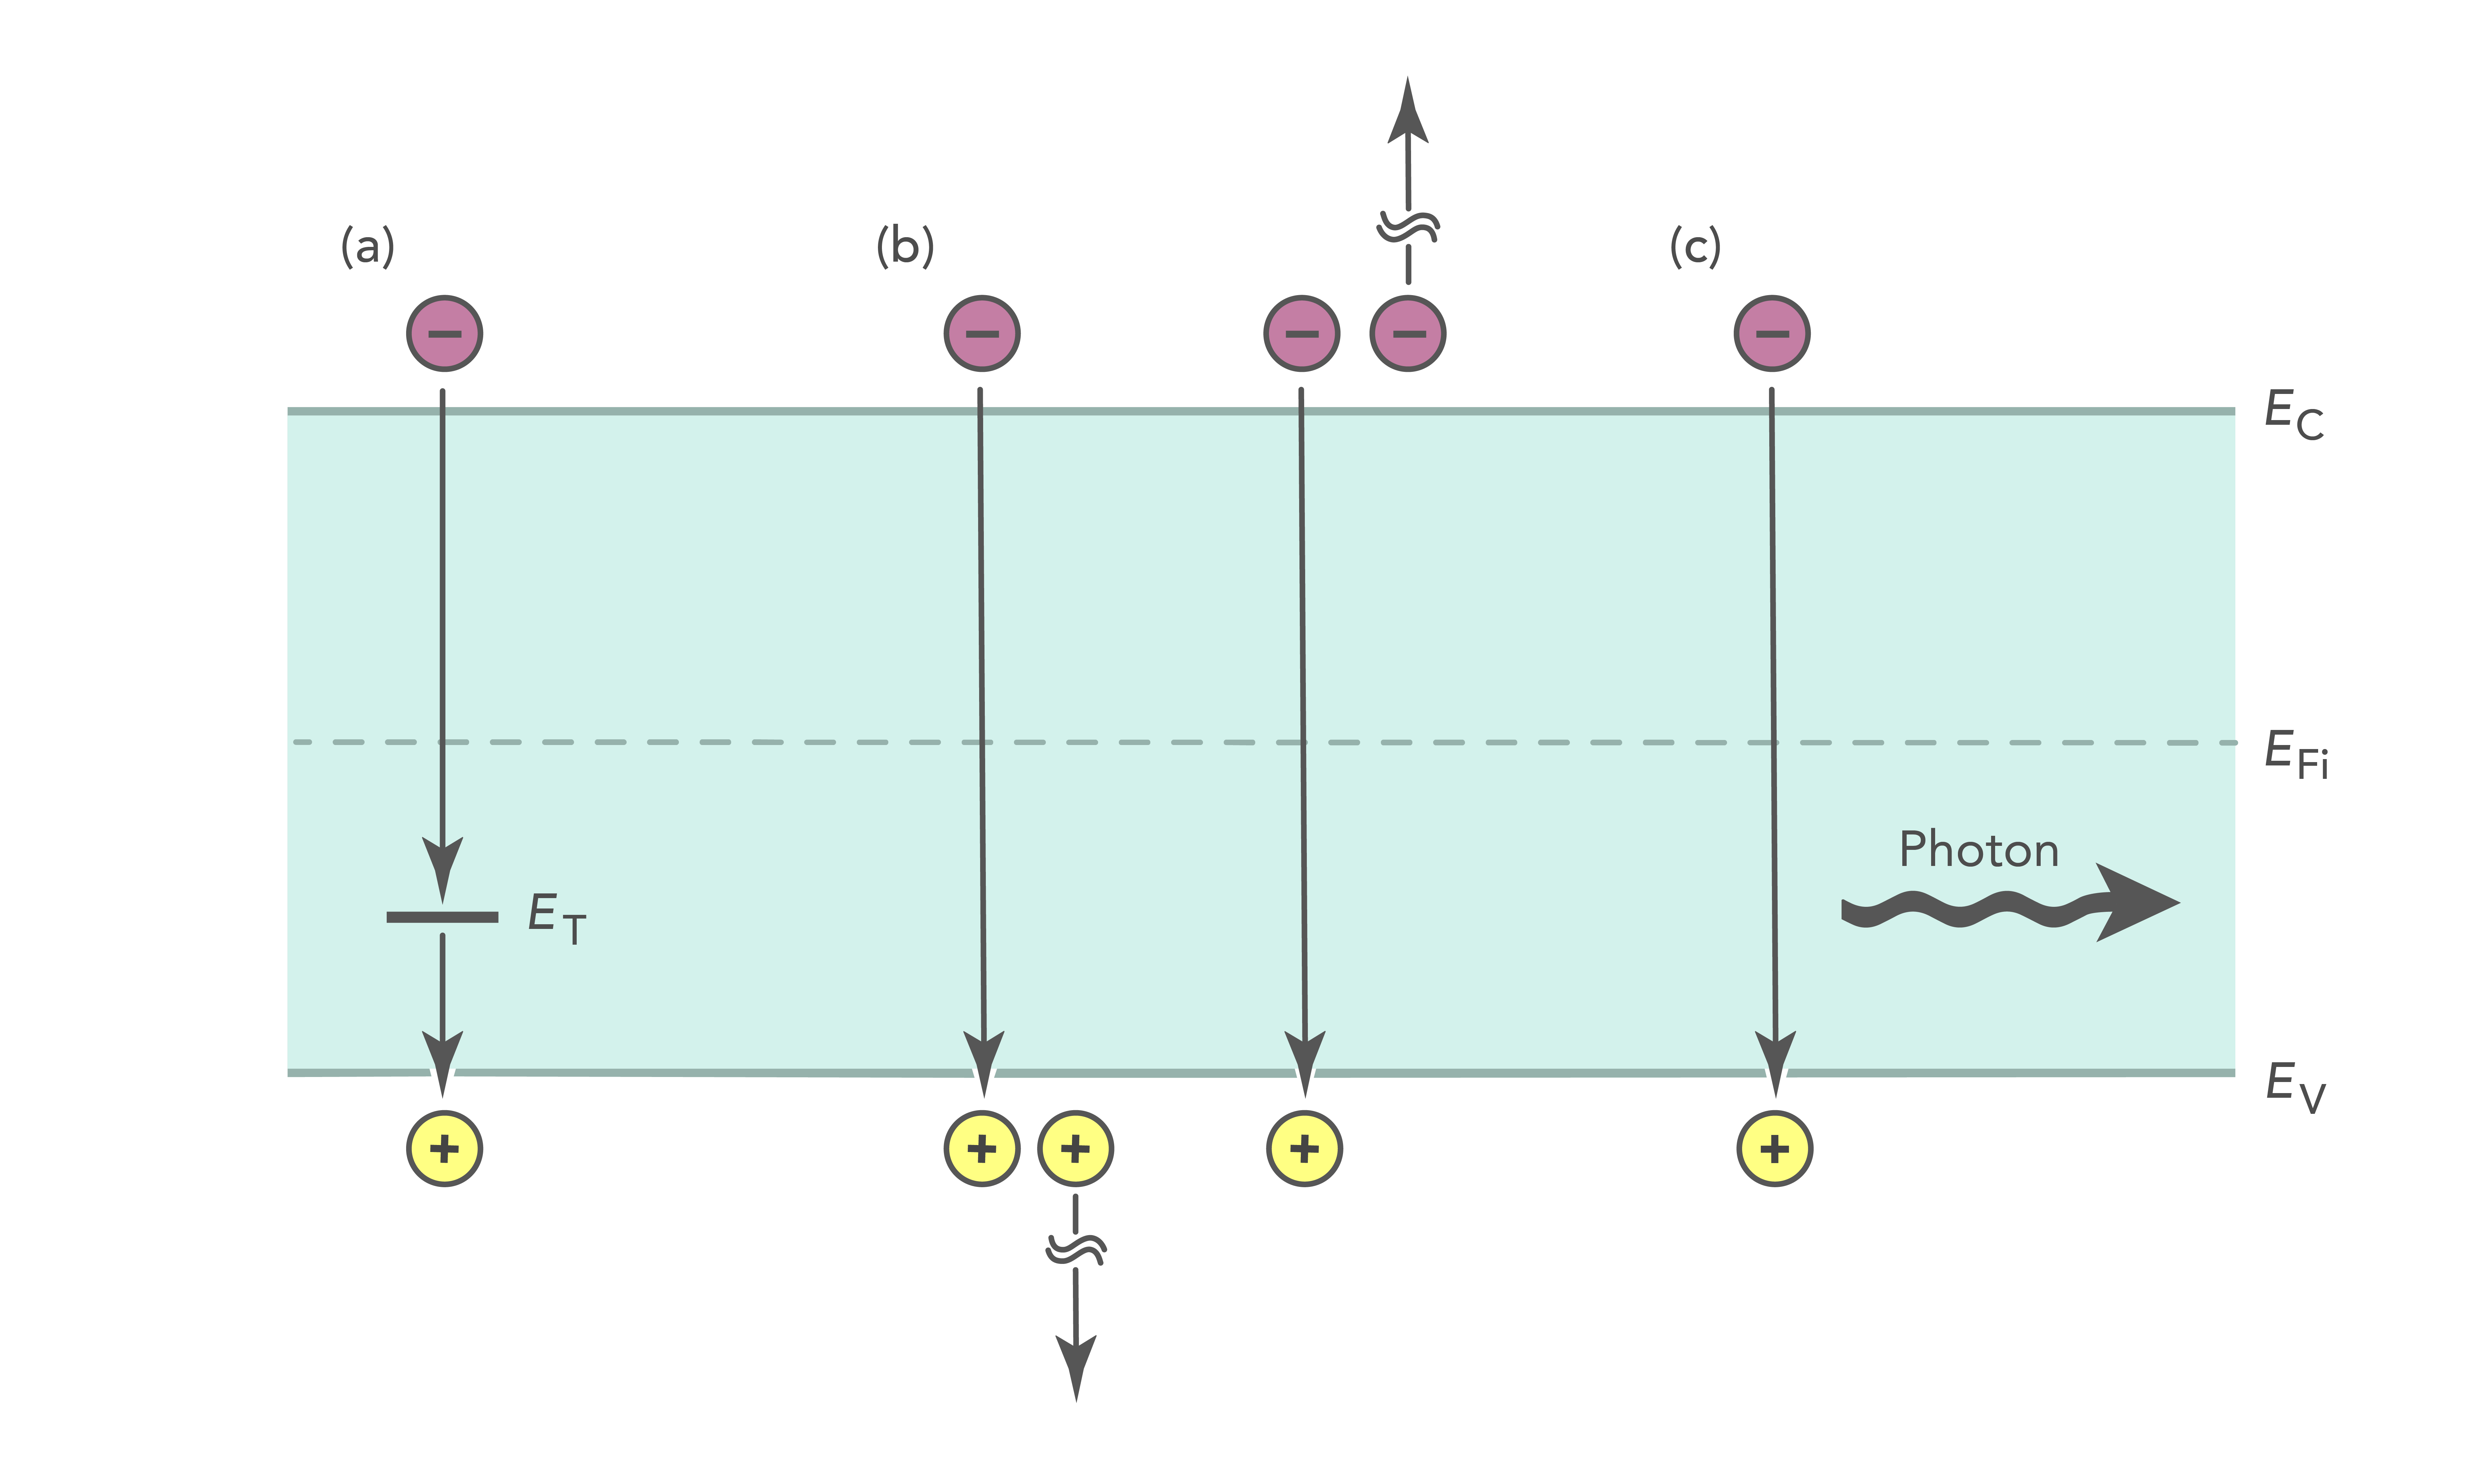
\includegraphics[width=\linewidth]{Bilder/rekbomChannels.png}
        \caption{Übersicht über die beteiligten Rekombinationsprozesse im ABC-Modell.}
        \label{fig:rekombChannels}
    \end{minipage}% <- sonst wird hier ein Leerzeichen eingefügt
\end{figure}
\noindent
%
Dazu werden drei Prozesse betrachtet: Zuallerst die nichtstrahlende Rekombination, die durch die Shockley-Read-Hall- (SRH-) Rekombination an Defekten beschrieben und durch den Parameter $A$ berücksichtigt wird ($R_{nonrad} = A \cdot n $). Sie ist linear abhängig von der Ladungsträgerdichte $n$. Sie findet statt unter der Beteiligung eines Defektniveaus und eines Phonons. Der strahlende Prozess der spontanen Rekombination ist für niedrige Ladungsträgerdichten quadratisch in $n$ und findet statt als Zwei-Teilchen Prozess bei dem Loch und Elektron beteiligt sind ($R_{rad} = B \cdot n^2 $). Dieser wird beschrieben mit dem Koeffizienten B. 
Der letzte Prozess ist die Auger-Rekombination der speziell für sehr hohe Anregungsleistungsdichten relevant ist und dann durch die kubische Abhängigkeit stark dominiert ($R_{auger} = C \cdot n^3 $). Dabei gibt ein bereits in das Leitungsband angeregte Elektron seine Energie an ein weiteres Elektron im Leitungsband ab. Dieses relaxiert dann entweder wieder zum Leitungsbandminimum unter Mitwirkung von Phononen oder verlässt bei Oberflächennähe den Kristall. Der letzte Fall bildet die Grundlage für die Auger-Elektronen-Spektroskopie.
Die effektive Rekombination ist somit die Summe aus der radiativen Rekombination, der nicht-radiativen Rekombination und der Auger-Rekombination.
\begin{equation}
    R_{eff} = R_{rad} + R_{nonrad} + R_{auger}
    \label{eq:iqe1}
\end{equation}
Der allgemein verwendete Ansatz zur Beschreibung der effektiven Rekombinationsrate $R_{eff}$ (oder auch Generationsrate $G$) wird mit Hilfe der genannten Koeffizienten beschrieben und beruht auf der Abhängigkeit der beteiligten Prozesse von der Ladungsträgerdichte $n$ und wird daher auch ABC-Modell genannt.
\begin{equation}
    R_{eff} (G) = A \cdot n + B \cdot n^2 + C \cdot n^3 
    \label{eq:iqe2}
\end{equation}
Weiter wird angenommen, dass die Anregungsleistungsdichte des Lasers P proportional zu
der Ladungsträger-Generationsrate G ist. Die radiative Rekombination $R_{rad}$ wird hauptsächlich beeinflusst durch den Überlapp der Wellenfunktionen von Elektronen und Loch im Leitungsband und Valenzband des QW. Dieser wiederum ist stark beeinflusst vom QCSE (Abb. 
\ref{fig:qcse}) und besonders bedeutend bei heteroepitaktisch gewachsenen Halbleiterstrukturen. 
%

	%
\section{Bestimmung der internen Quanteneffizienz}


Die aktive Region einer idealen LED würde für jedes injizierte Elektron jeweils ein Photon aussenden. 
Das bedeutet, die IQE die nach \cite{schub} wie folgt definiert ist
\begin{equation}
    IQE = \frac{ \footnotesize \text{Anzahl der Photonen die von der aktiven Zone emittiert werden pro Sekunde}}{ \footnotesize \text{Anzahl der Elektronen die in die LED injiziert werden pro Sekunde}}
\end{equation}
müsste den Wert $1$ annehmen. Die IQE kann somit analog beschrieben werden als Verhältnis von radiativer Rekombination und der effektiven Rekombination. Beschrieben mit Ratengleichungen und mit \ref{eq:iqe1} ist die IQE in ihrer einfachsten Form somit
\begin{equation}
    IQE = \frac{B \cdot n^2}{A \cdot n + B \cdot n^2 + C \cdot n^3} = \frac{R_{rad}}{R_{eff}}
\end{equation}
Die IQE kann mit Hilfe der Photolumineszenzspektroskopie bestimmt werden, in dem angenommen wird, dass keine thermisch aktivierten Defekte bei Raumtemperatur vorhanden sind
\begin{equation}
    A \propto e^{\frac{-E_{activation}}{kT}}
\end{equation}
Mit dieser und der Annahme das keine Auger Rekombination ($ C \cdot n^3 $) auftritt, ist die IQE bei Tieftemperatur ($ \propto 5K$) gleich 1. Somit kann die IQE beschrieben werden
\begin{equation}
    IQE = \frac{\text{Integrierte PL Intensität (T)}}{ \text{Integrierte PL Intensität } (T \rightarrow 0 K) }
\end{equation}
Als Quotient der integrierten PL Intensität bei Temperatur T und integrierter PL Intensität bei Tieftemperatur ($5K$). Die IQE ist folglich abhängig von der Temperatur, da der Paramater A für die SRH-Rekombination temperaturabhängig ist [Abb. \ref{fig:abha}]. 
Um also die IQE bei Raumtemperatur zu bestimmen, wird das Spektrum einer Probe bei 5K und 300K bei ansonsten möglichst gleichen Bedingungen aufgenommen. Die Intensität in Abhängigkeit der Wellenlänge wird interpoliert, dann integriert und dann das Verhältnis berechnet.
%
\begin{figure}[tb]
    \centering
    \begin{minipage}[t]{0.49\linewidth}
        \centering
        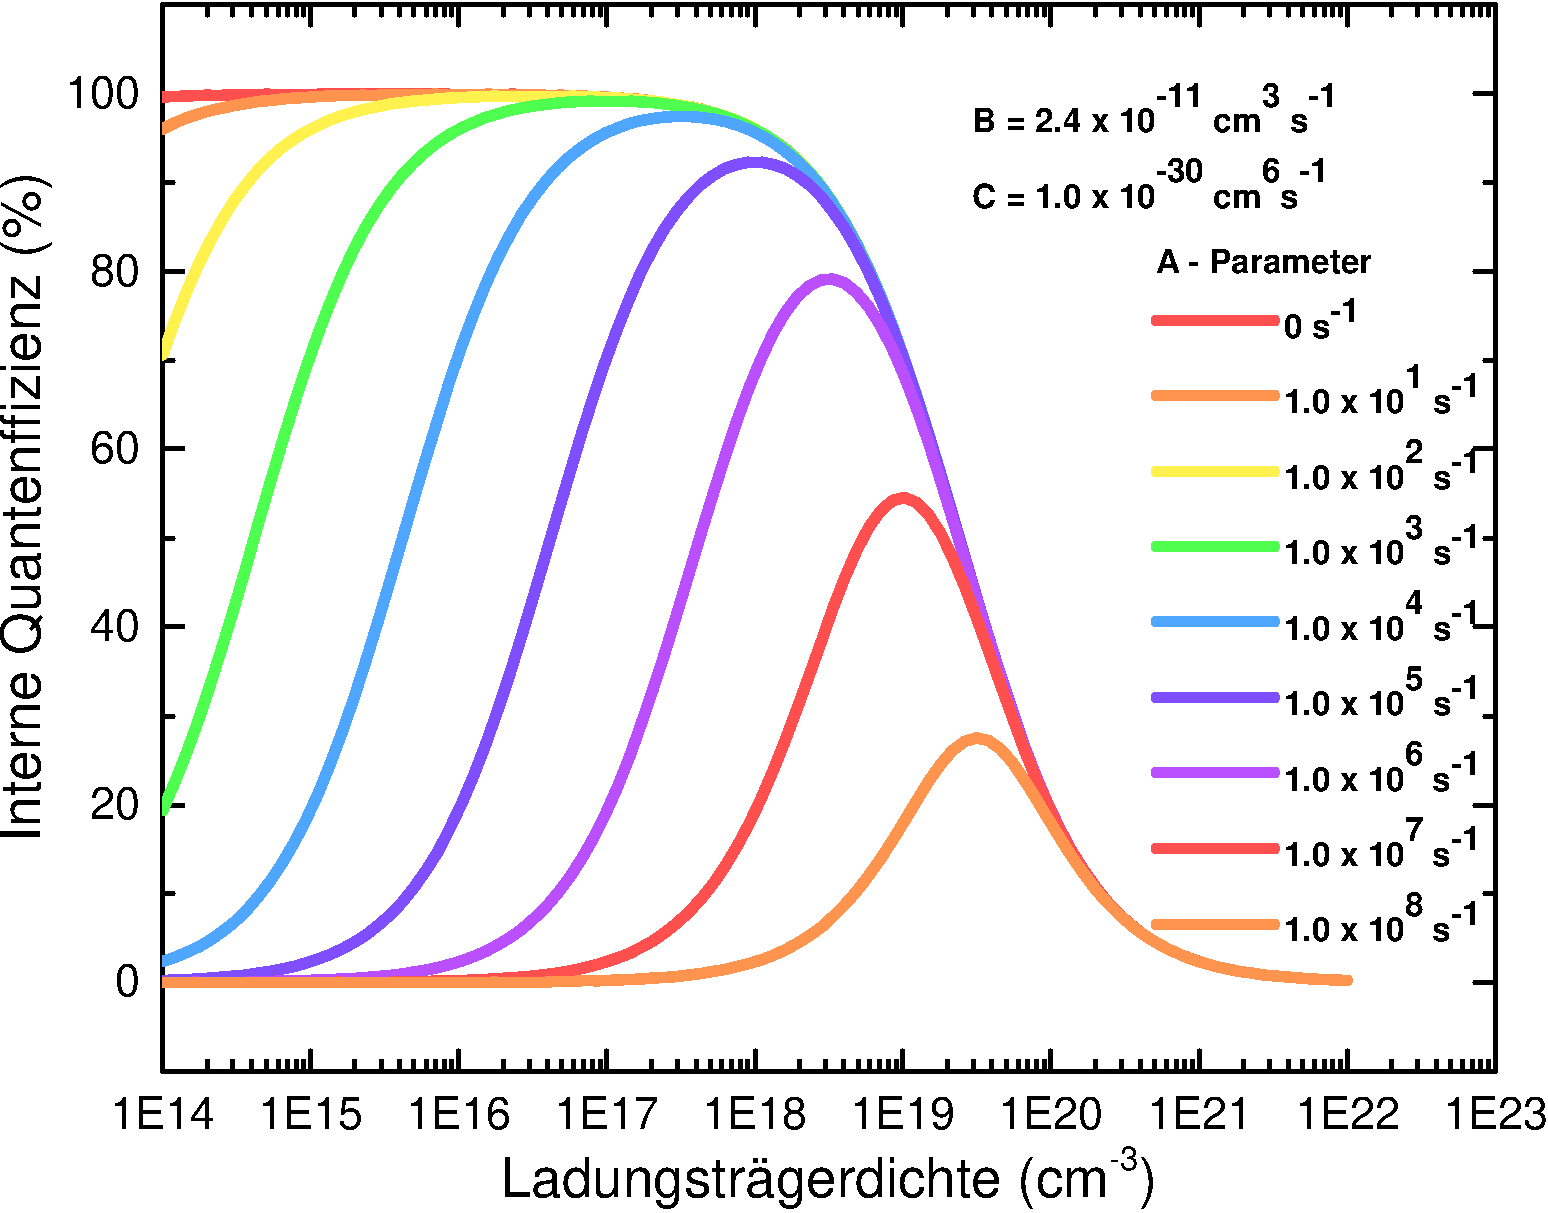
\includegraphics[width=\linewidth]{Bilder/IQEohneDotierungVerschAParams.pdf}
        \caption{Die Grafik zeigt die Abhängigkeit der internen Quanteneffizienz von der Ladungsträgerdichte für feste Paramater B und C. Der Paramater wird A wird variiert mit 9 verschiedenen Werten von $0 s^{-1} $ bis $10^9 s^{-1}$ ~\cite{semreich}.}
        \label{fig:abha}
    \end{minipage}% <- sonst wird hier ein Leerzeichen eingefügt
    \hfill
    \begin{minipage}[t]{0.49\linewidth}
        \centering
        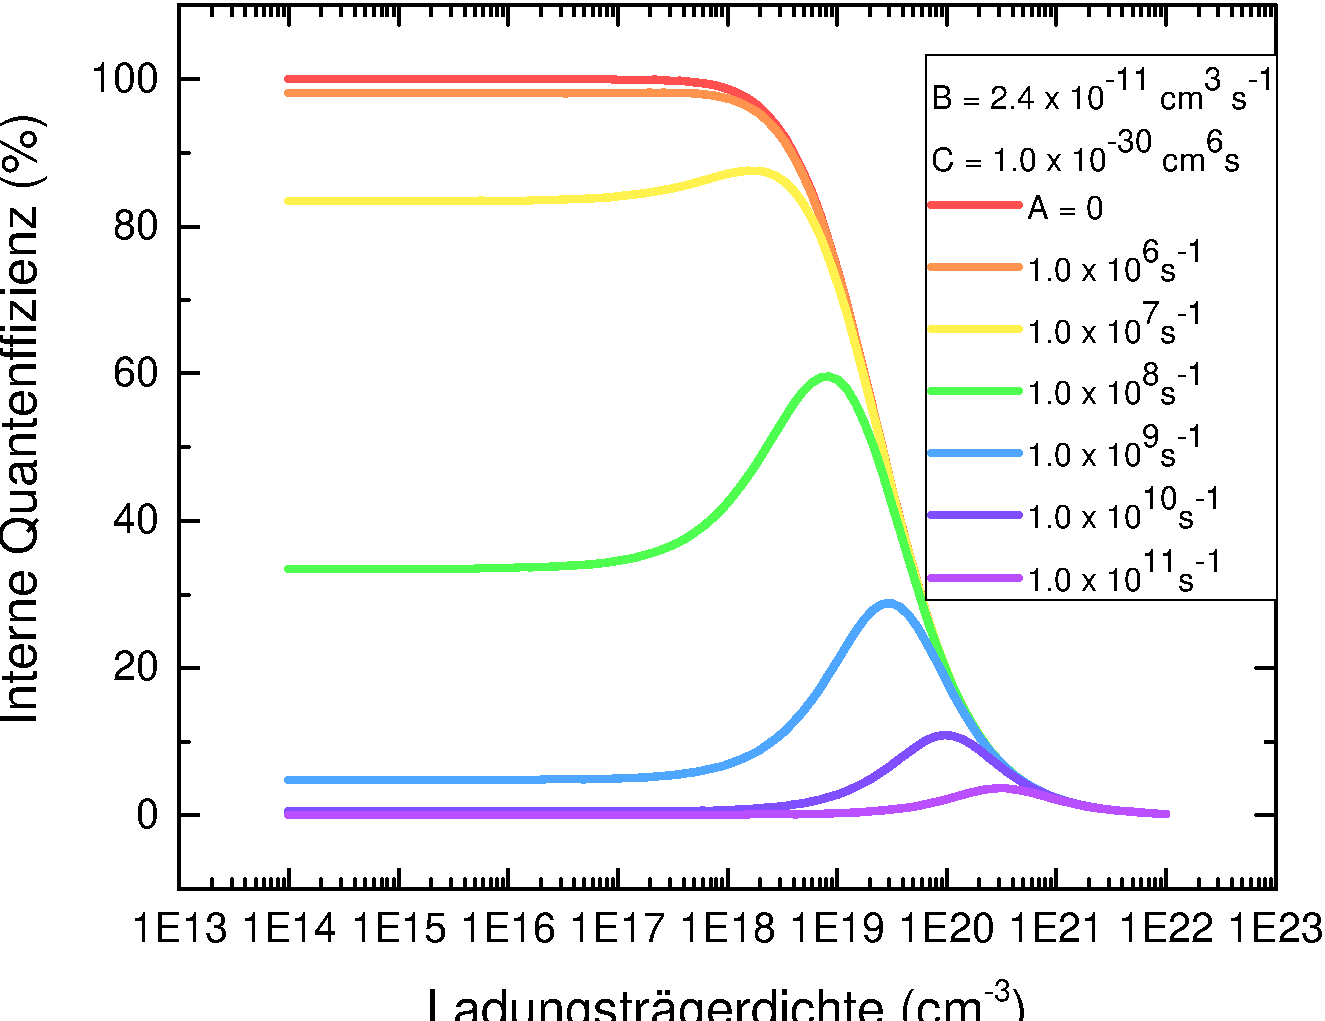
\includegraphics[width=\linewidth]{Bilder/IQEmitDotierungVerschAParams.pdf}
        \caption{}
        \label{fig:abha1}
    \end{minipage}
\end{figure}
\vspace{1cm}
\raggedright
\newpage
%
Das ABC-Modell stellt aber nur eine Vereinfachung dar und berücksichtigt nicht alle vorkommenden Effekte wie beispielsweise Lokalisierung, Screening durch Ladungsträger und Dotierung. 
Der Effekt der Dotierung spielt dabei eine besonders wichtige Rolle, da eine Silizumdotierung üblich in UV-Leds ist und einen großen Einfluss hat.
Nach \cite{schub} kann gezeigt werden, dass die Ratengleichungen, mit der Annahme einer Dotierung für die 
die Radiative Rekombination sich ändert und soll nun hergeleitet werden:
\\newline
Jeder dotierte oder undotiere Halbleiter hat zwei Arten von Ladungsträgern, Elektronen und Löcher.
Im Gleichgewicht, bedeutet ohne externe Anregung durch Absorption von Licht oder Injektion von Elektronen, ist das Produkt von Elektronen- und Lochkonzentration eine konstante Größe.
\begin{equation}
    n_0 \cdot p_0 = n_i^2
    \label{eq:constant}
\end{equation}
Hierbei sind $n_0$ und $p_0$ die Elektron- und Lochkonzentration unter Gleichgewichtsbedingung und $n_{i}$ damit die intrinsische Ladungsträgerkonzentration.
Werden zusätzlich die durch Anregung erzeugten Ladungsträger betrachtet, so ist die Gesamtladungsträgerkonzentration gegeben als Summe der Anregungs- und Gleichgewichtsladungsträger. 
\begin{equation}
    n_{ges} = n_0 + n \medspace \text{und} \medspace  p_{ges} = p_0 +  n 
\end{equation}
Hierbei sind $ n$ und $p$ die Anregungsladungsträger. 
Die Anzahl der stattfindenden Rekombination zwischen Elektronen und Löchern sind direkt proportional zur Elektronen-und Ladungsträgerkonzentration, so gilt, $R \propto n \cdot p $. Mit einer Proportionalitätkonstante, wird Rekombinationrate pro Zeit und Volumen definiert als
\begin{equation}
    R = - \frac{dn_{ges}}{dt} = - \frac{dp_{ges}}{dt} = B \cdot n_{ges} \cdot p_{ges}
\end{equation}
Weil Elektronen und Löcher bei Anregung paarweise erzeugt werden und verschwinden (durch Rekombination), gilt
\begin{equation}
    \label{eq:gleich}
    n(t) =  p(t)
\end{equation}
Die radiative Rekombinationrate wird dann mit $p_{0} = 0$ und Gleichung [\ref{eq:gleich}] zu
\begin{align}
\begin{split}
    R_{rad} &= B \cdot (n_0 + n)  \cdot (p_0 + p) ,
    \\
    R_{rad} &= B \cdot (n_0 + n) \cdot (n) ,
    \\
    R_{rad} &= B \cdot n^2 \cdot n \cdot n_0
\end{split}
\end{align}
Dabei beschreibt $n_{0}$ die Ladungsträgerkonzentration durch die Silizumdotierung. 
Somit wird die IQE zu:
\begin{equation}
    IQE = \frac{B \cdot n^2 + B \cdot n \cdot n_{0}}{A \cdot n + B \cdot n^2  + B \cdot n \cdot n_{0}+ C \cdot n^3} 
    \label{eq:dopediqe}
\end{equation}
Und hat einen enormen Einfluss auf die Ordinate, wie in Abb. [\ref{fig:abha1}] zu sehen ist.
%


	%
\section{Bestimmung der IQE bei Raumtemperatur durch Fitting}

\thispagestyle{fancy}

\begin{figure}[htb]
    \centering
    \begin{minipage}[t]{0.49\linewidth}
        \centering
        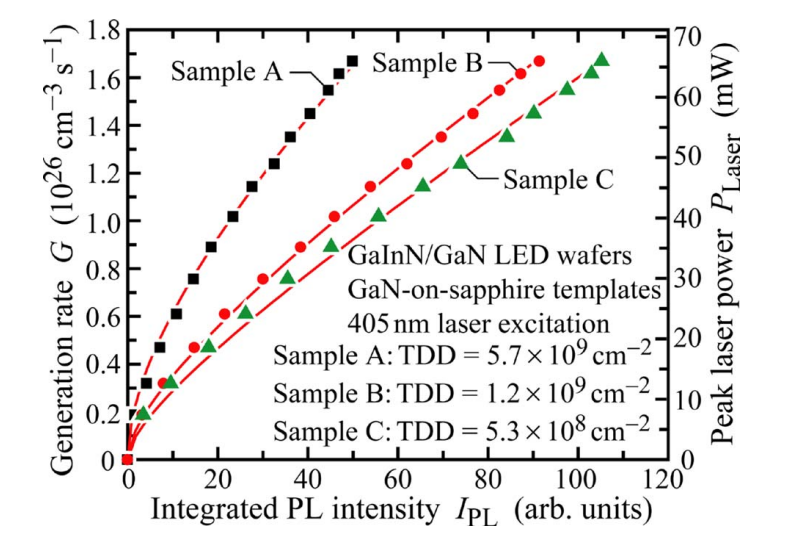
\includegraphics[width=\linewidth]{Bilder/raumtempMethodeBeispielFit.png}
        \caption{Fit für die Generationsrate in Abhängigkeit der integrierten PL-Intensität für drei InGaN/GaN MQW Proben mit einer unterschiedlichen Versetzungsdichten aus \cite{doi:10.1063/1.3100773}.}
    \end{minipage}% <- sonst wird hier ein Leerzeichen eingefügt
    \hfill
    \begin{minipage}[t]{0.49\linewidth}
        \centering
        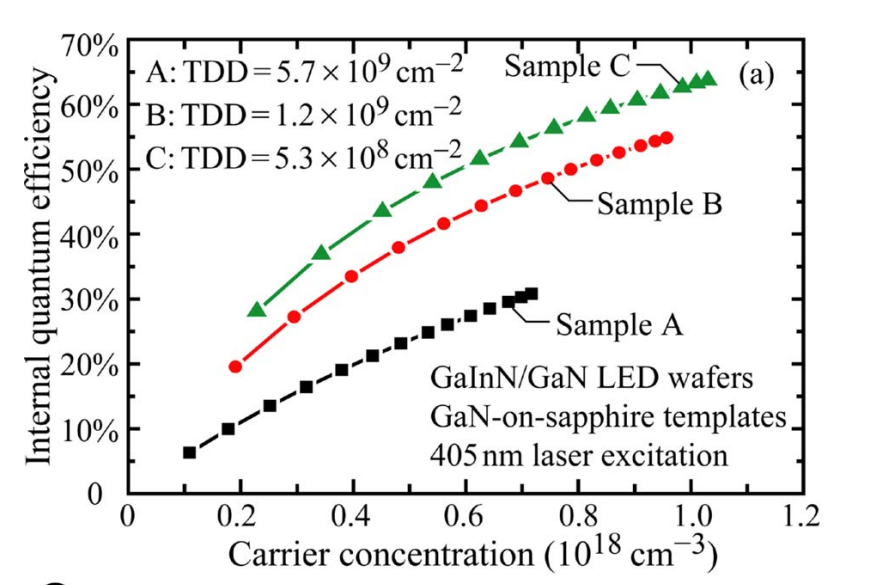
\includegraphics[width=\linewidth]{Bilder/raumtempMethodeIQE.png}
        \caption{Ergebnisse für die IQE in Abhängigkeit der Ladungsträgerdichte aus den durch die Fits extrahierten Werte ( \cite{doi:10.1063/1.3100773}). }
        \label{fig:iqert}
    \end{minipage}
\end{figure}
\noindent
In diesem Kapitel soll nun eine in \cite{doi:10.1063/1.3100773} und \cite{doi:10.1063/1.4917540} gezeigte Methode zur Bestimmung der IQE durch ein Fitting-Modell für die integrierte Intensität in Abhängigkeit der Ladungsträgerdichte vorgestellt werden. Das ist insbeondere von Vorteil, da so ein aufwändiges runterkühlen nicht mehr notwendig wäre, da die Spektren allein bei Raumtemperatur aufgenommen werden könnten. 
\newline
Angefangen mit der Rekombinationsrate, geht das Modell davon aus,
dass bei Raumtemperatur Auger-Rekombination nur bei sehr hohen Anregungsleistungsdichten relevant ist, wegen der kubischen Abhängigkeit der Auger-Rekombination von der Ladungsträgerdichte $n$. Die Generationrate G und die IQE bei Gleichgewichtsbedinungen ist somit:
\begin{equation}
    G = R_{eff} = A \cdot n + B \cdot n^2
    \label{eq:generationrate}
\end{equation}  
\begin{equation}
    IQE = \frac{B\cdot n^2}{A \cdot n + B \cdot n^2} = \frac{B\cdot n^2}{G}
    \label{eq:iqe2}
\end{equation}  
G beschreibt namentlich die Rate der Ladungsträger die durch Bestrahlung mit dem Laser erzeugt werden und entspricht hierbei der effektiven Rekombinationsrate $R_{eff}$.
Die integrierte PL-Intensität kann beschrieben werden als:
\begin{equation}
    I_{PL} = \eta \cdot B \cdot n^2
    \label{eq:integint}
\end{equation} 
$\eta$ ist eine konstante die durch das Volumen der angeregten aktiven Region und der Kollektionseffizienz bestimmt wird. Durch Eliminierung von $n$ in den Gleichungen \ref{eq:generationrate} und \ref{eq:integint} kann die Generationsrate durch die integrierte PL Intensität beschrieben werden
\begin{equation}
    G = \frac{A}{\sqrt{B\cdot n}}\sqrt{I_{PL}} + \frac{1}{\eta} I_{PL}
    %\label{eq:newgenrate}
\end{equation} 
Um dies in Zusammenhang mit dem Experiment zu bringen, kann die Generationsrate getrennt berechnet werden mit Nutzung experimenteller Werte durch 
\begin{equation}
    G = \frac{P_{laser} (1-R)\alpha l}{A_{spot} l h v} = \frac{P_{laser}(1-R) \alpha }{ (A_{spot} h v)}
   % \label{eq:newgenrate}
\end{equation} 
Dabei ist $P_{laser}$ die optische Leistung die auf der Probe landet, $R$ ist die Fresnel Reflektion auf der Probenoberfäche, $A_{spot}$ ist die Fläche des Laserspots auf der Probe, $h v$ ist die Energie eines Photons mit $193 nm$ und $\alpha$ ist der Absorptionskoeffizient. Damit ist es möglich, die Generationsrate zu bestimmen und in Abhängigkeit der integrierten PL-Intensität darzustellen. Und indem die Koeffizienten $c_1 = A \sqrt{B  \eta}$ und $c_2 = 1 / \eta$ durch einen Fit der Generationsrate in Abhängigkeit der integrierten Intensität extrahiert werden, kann die IQE bestimmt werden. Dazu wird $c_1$ nach A umgestellt ($A = \sqrt{B \eta} \cdot c1$) und in \ref{eq:generationrate} eingesetzt
\begin{equation}
    G = \sqrt{B \eta} \cdot c_1\cdot n + (\sqrt{B} \cdot n)^2
    \label{eq:generationrateneu}
\end{equation}  
Durch lösen von Gleichung \ref{eq:generationrateneu}, für $(\sqrt{B} \cdot n)$ und einsetzen in Gleichung \ref{eq:iqe2} ist es so möglich die IQE basierend auf einem Fit durch Raumtemperaturmessung in Abhängigkeit der Anregungsleistungsdichten zu bestimmen (Abb. [\ref{fig:iqert}]).

hallo


	\thispagestyle{fancy}


\chapter{Optische Polarisation und Valenzbandstuktur}
\label{chap:polgrund}
%
\begin{figure}[H]
    \centering
    \begin{minipage}[t]{0.49\linewidth}
        \centering
        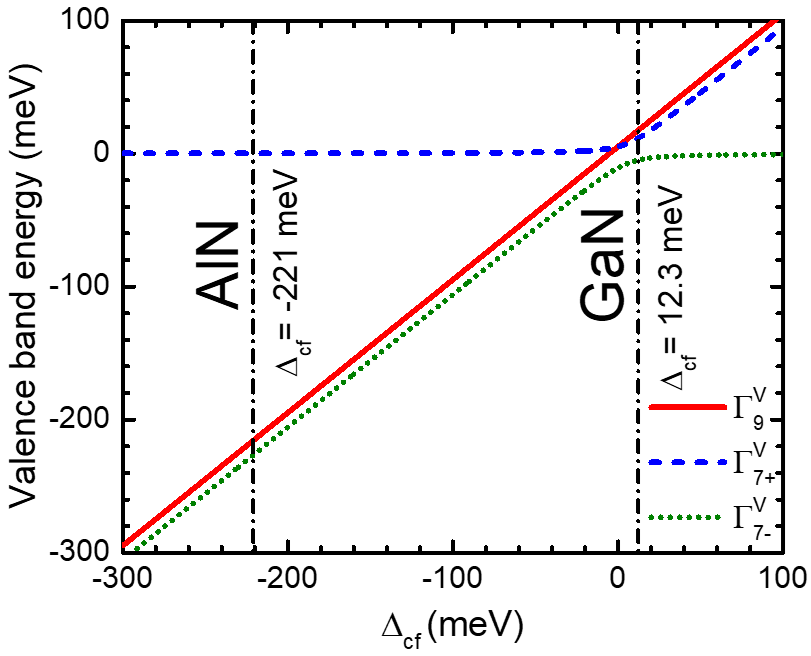
\includegraphics[width=\linewidth]{Bilder/vancebandPlot.png}
        \caption{Die energetische Reihenfolge der Valenzbänder in Abhängigkeit der Kristallfeldaufspaltung. Sichtbar ist der Wechsel der Bandanordnung mit sinkender Kristallfeldaufspaltung und der Effekt des "`anti-crossing"' bei den Bändern gleicher Symmetrie.    }
        \label{fig:auger5k}
    \end{minipage}% <- sonst wird hier ein Leerzeichen eingefügt
    \hfill
    \begin{minipage}[t]{0.49\linewidth}
        \centering
        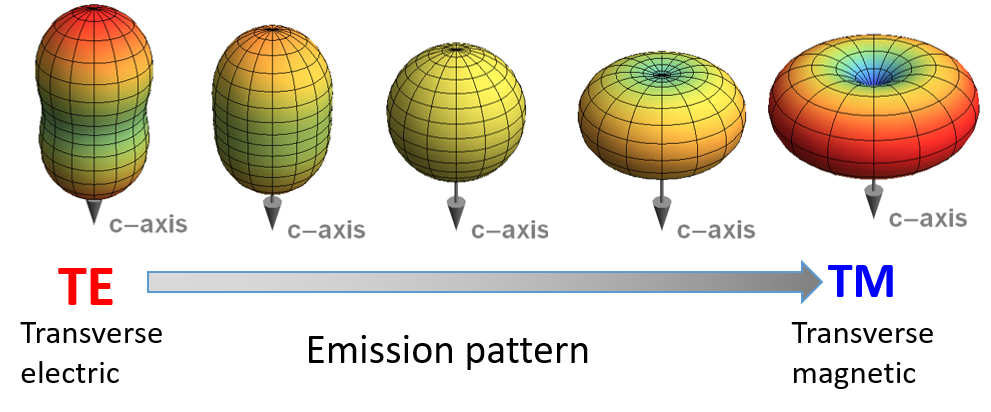
\includegraphics[width=\linewidth]{Bilder/martinTETM.png}
        \caption{Die Grafik zeigt die sich kontinuierlich ändernde Abstrahlcharakteristik in Abhängigkeit der Polarisation von TE- zu TM~\cite{martingut}.  }
        \label{fig:martintetm}
    \end{minipage}
\end{figure}
\vspace{0.1cm}
\noindent
Durch die Prozessierung und die Flip-Chip-Montage kann Licht nur durch die untere, unbewachsene Seite des Saphir-Substrates ausgekoppelt werden. Die Art und Weise der Lichtauskopplung hat einen bedeutenden Einfluss auf die Extraktionseffizienz und damit auf die externe Quantenffizienz(EQE). Durch die Geometrie bestimmt, hängt die Extraktionseffizienz maßgeblich vom Emissionsprofil ab, so dass Licht welches senkrecht zur Quantenfilmebene abgestrahlt wird, die höchste Extraktionseffizienz aufweist. 
Um diese zu optimieren, ist es wichtig die Bandstrukturen zu betrachten.
%
\begin{figure}[htb]
  \centering
  \begin{minipage}{\linewidth}
      \centering
        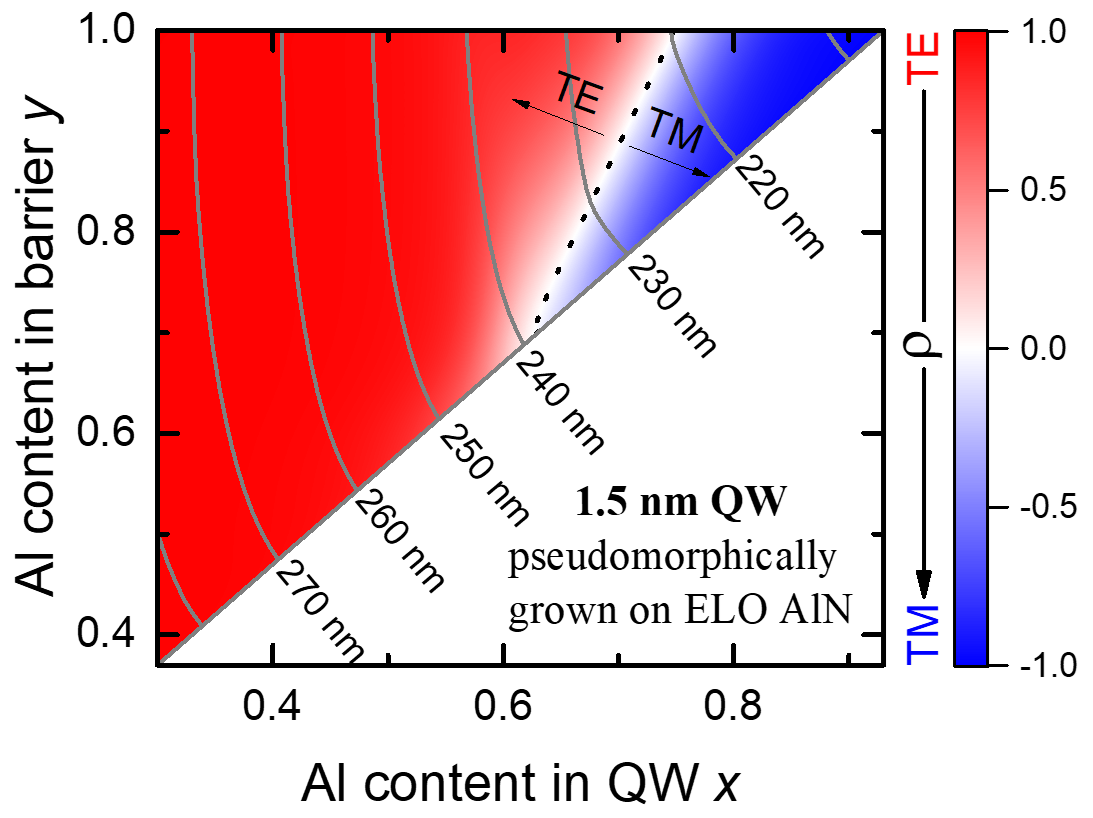
\includegraphics[width=0.6\textwidth]{Bilder/christophPolarisationSimu.png}
      \caption{Simulationsergebnisse des Polarisationsgrades in Abhängigkeit der Aluminiumkonzentration der Barrieren und QWs, basierend auf
dem k·p-Modell, für AlGaN-QW mit $1.5nm$-Dicke, die pseudomorph auf ELO-AlN gewachsen wurden. Die gestrichelte Linie zeigt, dass der Wechsel der Polarisation abhängig ist vom Aluminiumanteil in den Barrieren und QWs \cite{doi:10.1063/1.4932651} .}
      \label{fig:simuchr}
  \end{minipage}
\end{figure}
%
Die Valenzbandstrukturen von AlN und GaN unterscheiden sich durch die unterschiedliche anordnung der Bänder. Neben dem Leitungsband gibt es ein durch Spin-Bahn-Wechselwirkung und Kristallfeldenergie dreifach aufgespaltenes Valenzband~\cite{doi:10.1063/1.117689}. Sie werden nach ihrer energetischen Lage als A-,B- und C-Band bezeichnet. In AlN hat das A-Band eine $\Gamma^{L}_{7+}$, das B-Band eine $\Gamma^{L}_{9}$ und das C-Band eine $\Gamma^{L}_{7}$ Symmetrie. Bei GaN hingegen gilt folgende Reihenfolge:  $\Gamma^{L}_{9}$, $\Gamma^{L}_{7+}$, $\Gamma^{L}_{7}$. Die Ursache für den Symmetriewechsel liegt in der großen negativen Kristallfeldenergie von AlN mit einem Wert von $-221meV$ \cite{PhysRevB.87.235209} im Vergleich zur positiven von GaN mit $12,3meV$ ~\cite{PhysRevB.81.155202}. Bei Raumtemperatur wird, nach der Fermi-Dirac-Verteilung, das oberste Band mit der $\Gamma^{L}_{7+}$-Symmetrie, besetzt und aus Zuständen des $p_z$ bestehend, wird transversal magnetisch (TM) polarisiertes Licht emittiert ist. Die strahlende Rekombination findet demnach überwiegend mit Elektronen und Löchern aus dem A-Band mit $\Gamma^{L}_{7+}$-Symmetrie statt.
In GaN ist das oberste Valenzband am $\gamma$-Punkt mit $\Gamma^{L}_{9}$-Symmetrie . Das elektrische Feld des Lichtes ist senkrecht zur c-Kristallachse und wird durch Übergänge ins A- und B- Band erzeugt~\cite{doi:10.1063/1.3574025}, die aus Zuständen des $p_x$-und $p_y$-Orbitals bestehen. Bei strahlender Rekombination von Elektronen mit den Löchern im A- und B-Band entsteht also überwiegend TE-polarisiertes Licht ~\cite{doi:10.1063/1.3574025} . 
%
\begin{figure}[htb]
  \centering
  \begin{minipage}{\linewidth}
      \centering
      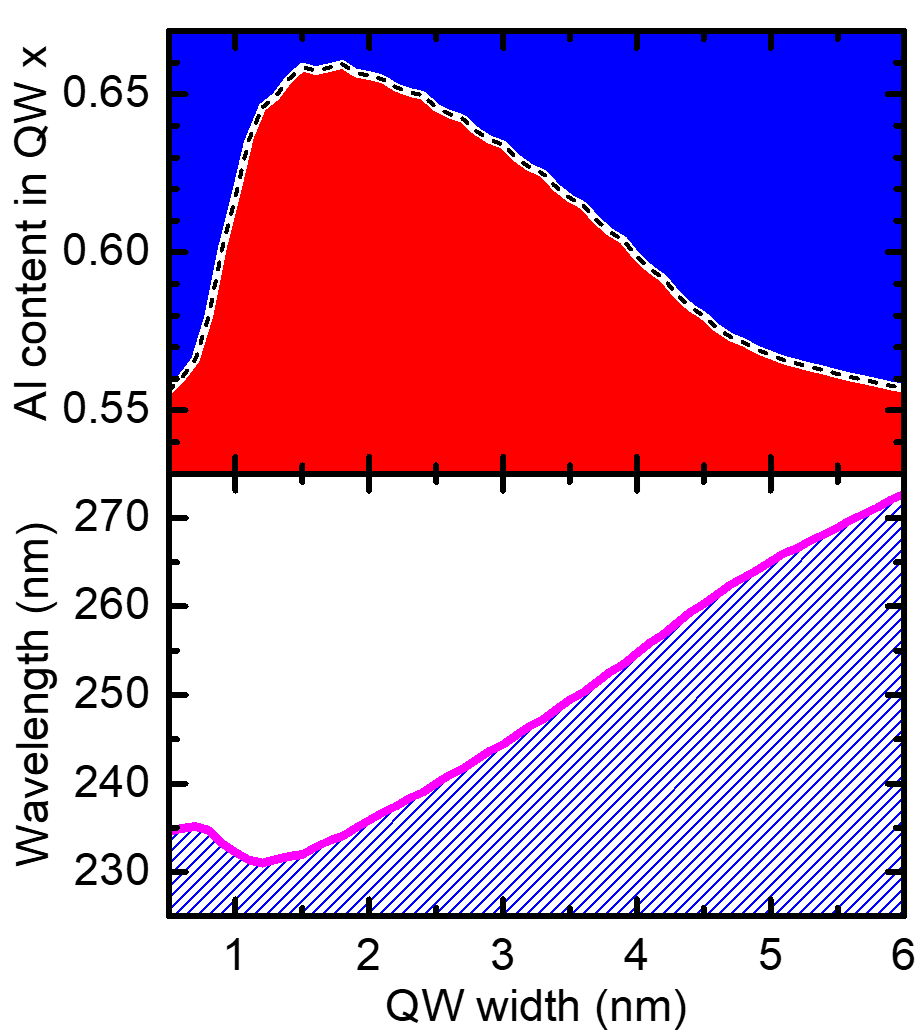
\includegraphics[width=0.4\linewidth]{Bilder/christophPolarisationSimu1.png}
      \caption{Ergebnisse der Simulation für die Polarisation in Abhängigkeit von der QW-Dicke(Wellenlänge) und dem Al-Gehalt in den QWs ~\cite{doi:10.1063/1.4932651}.}
      \label{fig:simu1chr}
  \end{minipage}
\end{figure}
%
Licht kann nicht ausgekoppelt werden, da es nur in der x-y- Ebene (parallel zur Quantenfilmebene) emittiert. Daraus resultierend sinkt die Extraktionseffizienz und damit die EQE. Bei $Al_{x}Ga_{1-x}N$ kommt es mit steigendem Aluminiumgehalt zu einer kontinuierlichen Verschiebung der Valenzbänder und es kommt zum sog. "`anti-crossing"' des $\Gamma^{L}_{7+}$ und $\Gamma^{L}_{7-}$ und resultiert in einer Änderung der Oszillatorstärke und damit der Polarisationseigenschaften ~\cite{doi:10.1063/1.4932651}.
Bedeutet, die Lichtemission ändert sich von hauptsächlich TE-polarisiertem Licht zu TM-polarisiertem Licht. Der genaue Aluminiumgehalt, an dem die Valenzbandkreuzung auftritt, ist noch nicht hinreichend bekannt. Theoretische Betrachtungen sagen für unverzerrtes $Al_{x}Ga_{1-x}N$ einen Kreuzungspunkt bei ca. $7\%$ vorher ~\cite{doi:10.1063/1.3675451}. Durch den starken Einfluss von Verzerrungen auf die Energie der  Valenzbandkante, ist die Polarisation abhängig von der wachsenden biaxialen Verzerrung bei steigendem Aluminiumgehalt. So wurde von Kawanishi et al. experimentell der Wechsel bei einem Aluminiumgehalt von "`75\%"' festgestellt ~\cite{doi:10.1063/1.2410242}. 
Noch dazu ist ist die Polarisation bei Mehrfachquantenfilmen(engl. multiple quantum wells, kurz MQW) abhängig vom Ladungsträgereinschluss (engl. quantum confinement). Dieser ist hauptsächlich bestimmt durch die Barrierenhöhe und Barrierendicke. Mit kleiner werdender Barrierendicke, steigt der Grad der Polarisation durch den gesteigerten Einfluss des QCSE ~\cite{PhysRevB.84.035305}. 
Reich et al. untersuchte unter diesem Zusammenhang die optische Polarisation der Emission von UVC-Leuchtdioden(LEDs) auf Basis von (0001) orientierten $Al_{x}Ga_{1-x}N$-MQWs mit Simulationen und Elektrolumineszenzmessungen ~\cite{doi:10.1063/1.4932651}. Dabei stellte er fest, dass mit zunehmendem Aluminium-Gehalt in den QWs die inplanare-Intensität des TE polarisierten Lichtes gegenüber dem des TM polarisierten Lichts abnimmt, was auf die Neuordnung der Valenzbänder in $Al_{x}Ga_{1-x}N$ zurückzuführen ist. 
Durch Modellrechnungen, basierend auf dem k·p-Modell, wurde die Abhängigkeit der Polarisation von den Aluminiumkonzentration in den Barrieren und QWs für pseudomorph aufgewachsenes ELO-AlN berechnet Abb. [\ref{fig:simuchr}]. Zusätzlich wurde die Polarisation in Abhängigkeit einer Variation der QW-Dicke und dem Al-Gehalt in den QWs betrachtet Abb. [\ref{fig:simu1chr}].
\begin{figure}[htb]
  \centering
  \begin{minipage}{\linewidth}
      \centering
      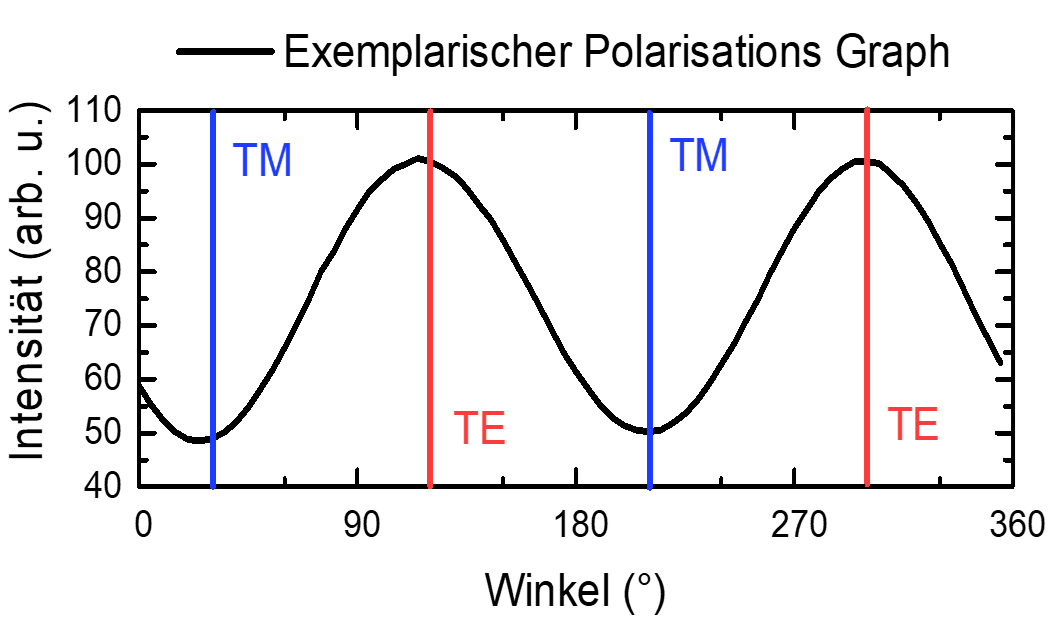
\includegraphics[width=0.6\linewidth]{Bilder/exemplPolGraph.png}
      \caption{Exemplarischer Graph einer Polarisationsmessung mit Photolumineszenzspektroskopie. Zu sehen ist die integrierte Intensität in Abhängigkeit des Winkels eines Polarisators. Zur Bestimmung des Polarisationsgrades wird die integrierte Intensität der TM-Emission(Blau) $I_{T;}$  und der TE-Emission(Rot) $I_{TE}$ in Gleichung ~\ref{eq:pol} eingesetzt.}
      \label{fig:degra}
  \end{minipage}
\end{figure}
Diese Erkenntnise lassen sich zusätzlich mit Hilfe der Photolumineszenz prüfen. So lässt sich die Polarisation bestimmen, in dem die Polarisation $\rho$ der Photolumineszenzemission aus der Kante einer Probe mit Hilfe der Gleichung 
\begin{equation}
\rho = \frac{ I_{TE} - I_{TM} }{ I_{TE} - I_{TM} } 
\label{eq:pol}
\end{equation}
bestimmt wird. Dabei ist $I_{TE}$ die integrierte Intensität der TE-polarisierten und $T_{TM}$ die Intensität der TM-polarisierten Emission. 
 



	%
\chapter{Aufbau}


\thispagestyle{fancy}
\label{chap:aufbau}
\section{Photolumineszenzaufbau}
\begin{figure}[!htb]
    \centering
    \begin{minipage}[t]{\linewidth}
        \centering
        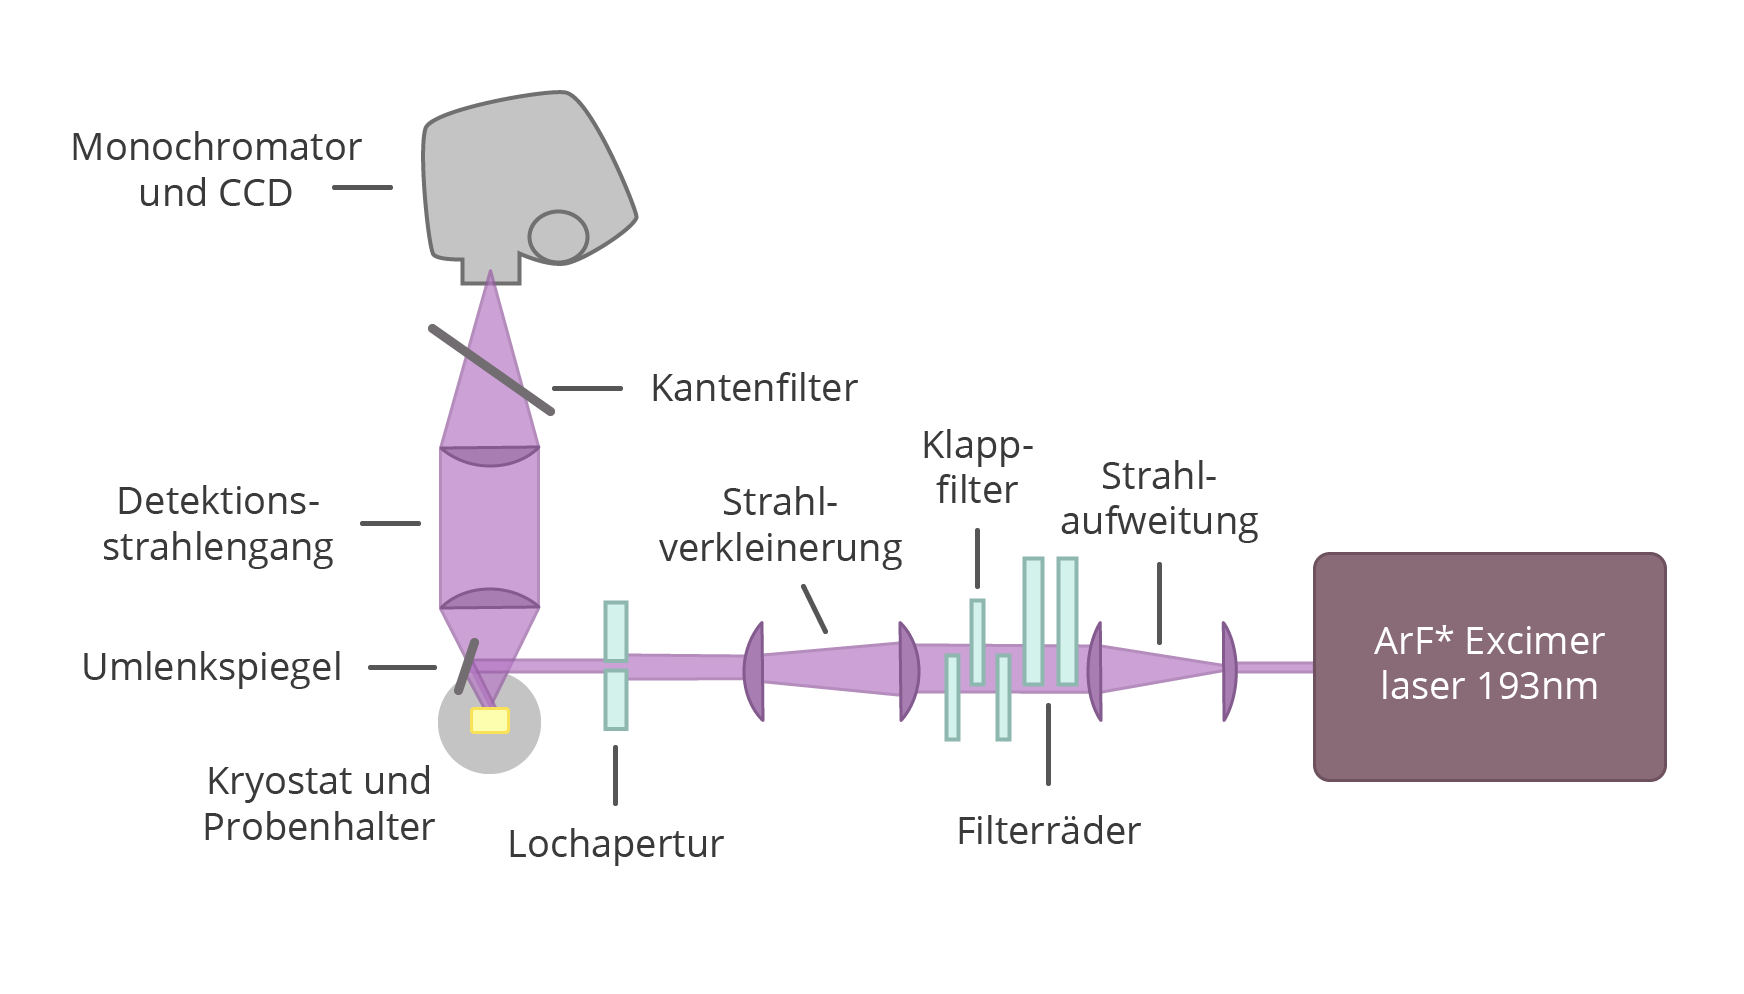
\includegraphics[width=0.8\linewidth]{Bilder/aufbauPL.png}
        \caption{Aufbau des Photolumineszenzmessplatzes der AG Kneissl. }
        \label{fig:plaufbau}
    \end{minipage}% <- sonst wird hier ein Leerzeichen eingefügt
\end{figure}
\noindent
Für die experimentelle Untersuchung der UV-Photolumineszenz wurde der PL-Aufbau der AG-Kneissl, der in Abbildung \ref{fig:plaufbau} dargestellt ist, verwendet. Der PL-Aufbau wurde von Christoph Reich in der Zeit seiner Diplomarbeit aufgebaut und während seiner Promotion erweitert \cite{creich}. 
Als Anregungsquelle für die Photolumineszenz dient ein ArF-Excimerlaser mit einer Wellenlänge von $193 \ nm$ ($6,4 \ eV$). Mit dieser Wellenlänge ist er bestens geeignet für die Überbandanregung von Nitridhalbleitern. 
Des Weiteren bietet der Aufbau die Möglichkeit von temperaturabhängigen Untersuchungen von $5 \ K $ bis $300 K$. Dies ist auch die Grundlage für die Bestimmung der IQE. 
\newline
Der Laser mit dem Modellnamen "`Xantos XS"' von der Firma Coherent bietet eine maximale Emissionsenergie von $ 5 \ mJ $ und eine einstellbare Frequenz bis zu 500 Hz bei einer Pulsdauer von $5 \ ns$.
Durch interne Rückkopplung ist eine Energiestabilisierung möglich, die die Schwankung der Anregungsleistung auf 3 Prozent minimiert. 
\newline
Die Ansteuerung des kompletten Messvorgangs erfolgt durch die Messsoftware von Christoph Reich, entwickelt in der grafischen Programmiersprache "`LabView"' von Texas Instruments. Diese ermöglicht alle nötigen Einstellungen an Pumpen, Heizern, Laser, Filtern und Spektrometer, um einen nahezu komplett automatisierten Messvorgang zu starten. Spektren können so mit verschiedenen Parametern wie Position, Anregungsleistungsdichte, Temperatur, Energiebereich und Integrationszeit aufgenommen werden und auch ein Gaswechsel ist möglich.
\newline
Beginnend vom Laser wird im ersten Schritt der Laserstrahl durch ein Linsensystem, bestehend aus einer Zerstreuungs- und Sammellinse, aufgeweitet. Dieser Schritt ermöglicht es, die Anregungsleistungsdichte zu verringern, um die am Aufbau beteiligten Geräten, insbesondere die Filterräder, nicht mit zu hohen Leistungen zu beschädigen. Mit Hilfe der Filterräder ist es möglich, die Anregungsleistungsdichte 61 stufig zu variieren und somit leistungsdichteabhängige IQE Messungen zu machen. Als nächstes passiert der Strahl ein Linsensystem aus zwei Sammellinsen für eine Strahlverkleinerung. Vor dem Auftreffen des Strahles am Probenhalter im Kryostaten passiert der Strahl noch eine Lochblende. Sie dient der Entfernung achsennaher Strahlen und um bei Bedarf den Strahldurchmesser noch weiter zu verringern. 
\newline
Um den Strahl in Richtung des Probenhalters durch das Fenster im Kryostaten zu lenken, wird ein Spiegel mit einer dielektrischen Beschichtung benutzt. Der Laserstrahl durchdringt die Fenster des Kryostaten, welche speziell für eine hohe Transmission in diesem Wellenlängenbereich ausgelegt sind. Der Kryostat selbst ist horizontal und vertikal verschiebbar, um die Messung mehrerer Proben im Probenhalter in einem Messvorgang bei gleichen Bedingungen zu ermöglichen. Die Proben werden mit einem Kleber auf dem Probenhalter selbst befestigt, bevor dieser in den Kryostaten geschoben wird. 
Die Anregung der Proben mit dem Laserstrahl führt zur probenspezifischen Emission von Licht. Diese wird von einer Linse im Strahlengang vor dem Detektor eingefangen und von einer zweiten Linse auf den Monochromatorspalt fokussiert.
\newline
Bei dem Monochromator handelt es sich um einen "`iHR 320"' des Herstellers "`Horiba"'. Zur Verfügung stehen drei Blazegitter mit $300 \thinspace \frac{Linien}{mm}$,
$600 \thinspace \frac{Linien}{mm}$ und $1800 \thinspace \frac{Linien}{mm}$. Bei der verwendeten Spaltbreite von $100 \thinspace \mu m$ entspricht die maximale Auflösung in etwa $5 \thinspace meV$ ($0,17 \thinspace nm$). Für Messungen oberhalb von $225 \thinspace nm$ besteht die Möglichkeit einen Kantenfilter in den Strahlengang einzubringen, mit dem das Laserstreulicht und dessen höhere Ordnungen aus dem Spektrum entfernt werden können. Bei dem CCD Chip handelt es sich um das Modell "`Syncerity"' von "`Horiba"' der "`open electrode"' -Bauart mit 1024x256 einzelnen Pixeln. 

\section{Messaufbau Lichtpolarisation}
\begin{figure}[!htb]
    \centering
    \begin{minipage}[t]{\linewidth}
        \centering
        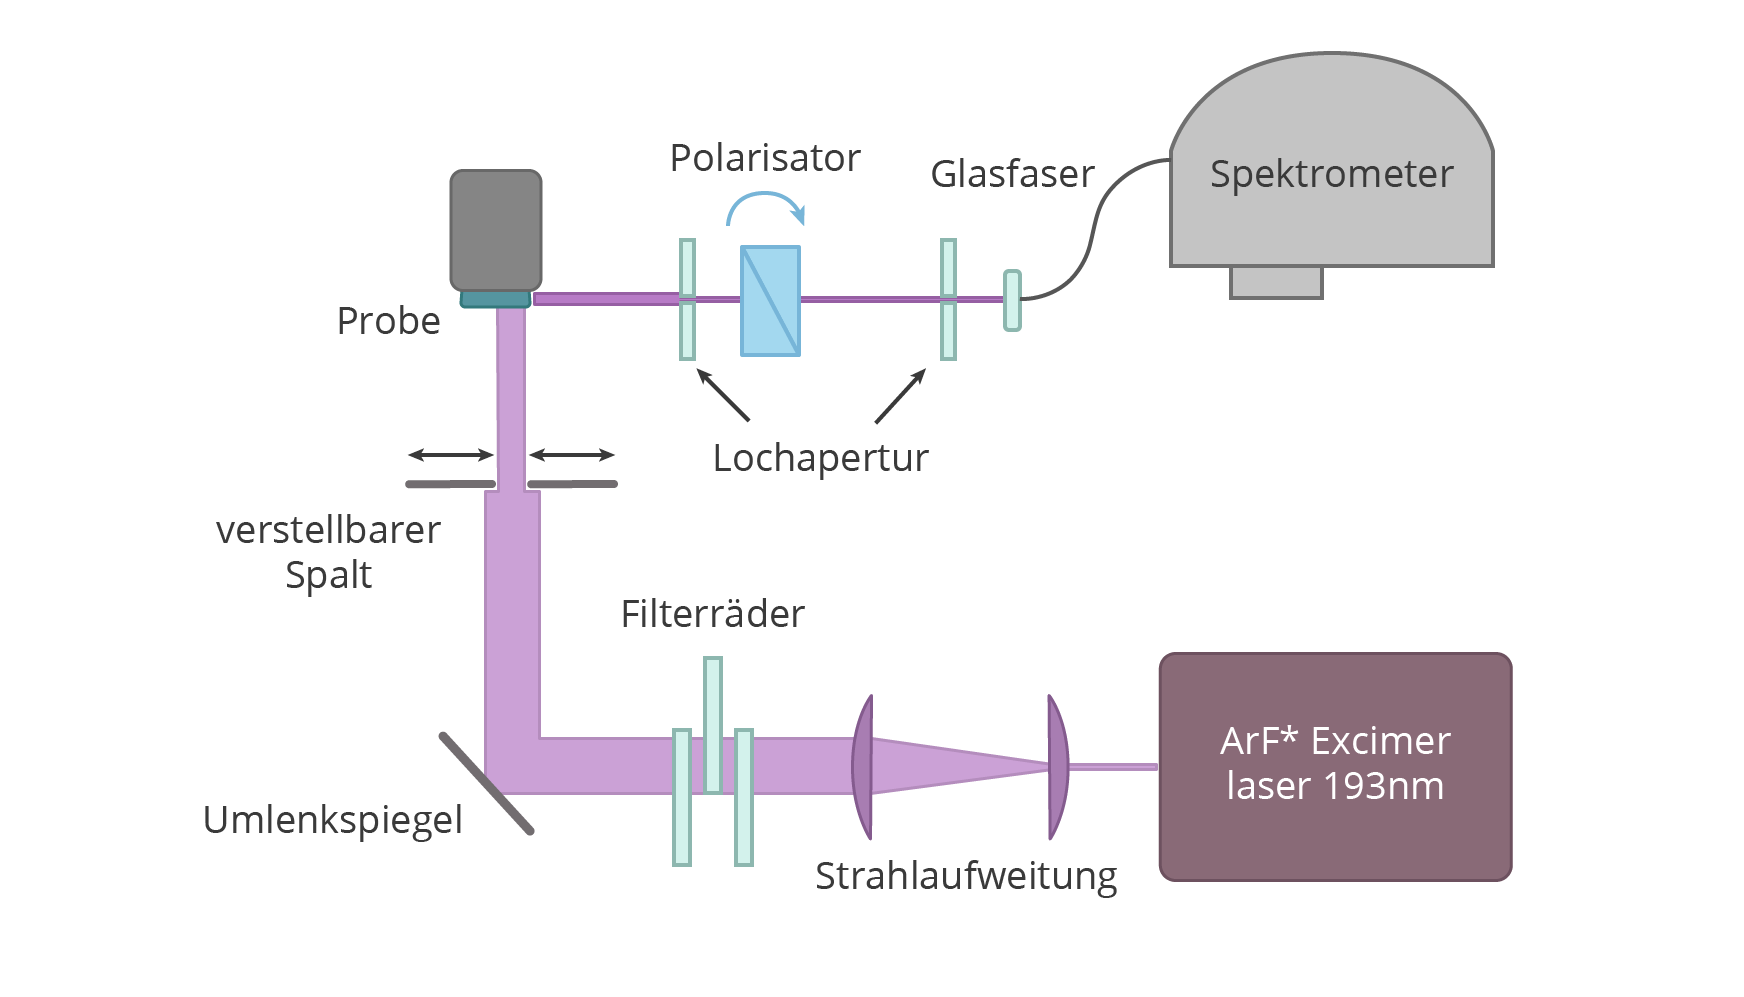
\includegraphics[width=0.8\linewidth]{Bilder/aufbauPol.png}
        \caption{Aufbau des Photolumineszenzmessplatzes der AG Kneissl zur Bestimmung der Polarisation. }
        \label{fig:polaufbau}
    \end{minipage}% <- sonst wird hier ein Leerzeichen eingefügt
\end{figure}
\vspace{1cm}
\noindent
Der Messaufbau zur Bestimmung der Lichtpolarisation ist in Abbildung \ref{fig:polaufbau} dargestellt.
Die Anregung der untersuchten Proben erfolgt senkrecht zur Probenoberfläche. Die Lumineszenz der Probe wird aus der Kante gemessen, weil TM-polarisiertes Licht nur vertikal zur c-Achse, wie in Abbildung \ref{fig:martintetm} sichtbar, emittiert wird. Die Lumineszenz wird dann unter kleinem Öffnungswinkel über eine Linse mit sich dahinter befindlicher Blende eingesammelt und parallelisiert. Das parallelisierte Licht wird dann durch einen Glan-Taylor-Polarisator geleitet. Dass das Licht parallelisiert ist, ist wegen der anisotropen Brechzahl des Polarisators wichtig. Diese ist neben der Polarisationsrichtung auch von dem Eintrittswinkel abhängig und entscheidet ob der Strahl transmittiert oder reflektiert wird \cite{0950-7671-25-12-304}. In Abhängigkeit der Orientierung des Polarisators wird TE- oder TM-polarisiertes Licht transmittiert. Der eingestellte Winkel lässt sich $1^\circ$ granular einstellen. 

	%\chapter{Aufbau: Erweiterung und Bestimmung der Degradation des UV Quarzglases }
\thispagestyle{fancy}

\section{Bestimmung der Degradation des UV Quarzglases}
%
\begin{figure}[htb]
  \centering
  \begin{minipage}[t]{0.49\linewidth}
      \centering
      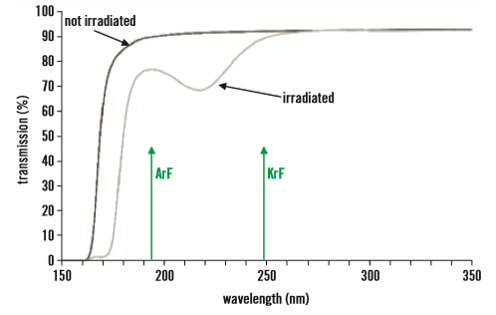
\includegraphics[width=\linewidth]{Bilder/uvsilicaDegradation.png}
      \caption{Vom Hersteller angegebene wellenlängenabhängige Transmission vor und nach Degradation durch Bestrahlung.}
      \label{fig:degra}
  \end{minipage}
\end{figure}
\vspace{1cm}
\raggedright
Da die Messung der Anregungsleistungdichte erfolgt, bevor das Laserlicht die Probe durch das UV-Quarzglas im Kryostaten trifft, ist es wichtig den Transmissionsverlust zu bestimmen, um die realen Werte für die Anregungsleistungsdichte zu kennen (Die Anregungsleistungsdichte die bei der Probe ankommt). Der Kryostat besitzt vier Fenster, bestehend aus UV-Quarzglas, das besonders transparent im UV-Wellenlängen bereich ist. Durch diese Fenster dringt das Laserlicht in den Probenhalter ein. Von diesen Fenstern war und ist eines in dauerhaftem Gebrauch. Wie in Abb. ~\ref{fig:degra} zu sehen ist, weisen die Fenster aber mit der fortlaufender Bestrahlung Degradation auf, so nimmt laut Hersteller durch Degradation die Transmission von 90 Prozent bis auf ca. 75 Prozent ab für eine Wellenlänge von 193 nm.
Um nun den Transmissongrad zu bestimmen, wurde der Probenhalter aus dem Kryostat entfernt, damit das Laserlicht ungehindert durch zwei parallel liegende Fenster durchdringen kann, um so auch die Anregungsleistungsdichte des Laserlichtes nach durchdringen des letzten Fenster messen zu können. So konnte die Anregungsleistungsdichte vor dem Eintreten und nach dem Austreten in den Kryostaten bestimmt werden. 
Dies wurde einmal bei den parallel liegenden unbenutzten Fenstern gemacht. Davon ausgehend, dass beide Fenster, da unbenutzt, den gleichen Transmissionsgrad haben, kann darauf zurückgeschlossen werden, dass ein unbenutztes Fenster einen Transmissionsgrad von 59 Prozent aufweist, was um ca. 10 Prozent von der Herstellerangabe abweicht, die aber nicht die Reflektion im Kryostaten mitberechnet. 
%
\begin{figure}[htb]
  \centering
  \begin{subfigure}{0.40\textwidth}
    \centering
    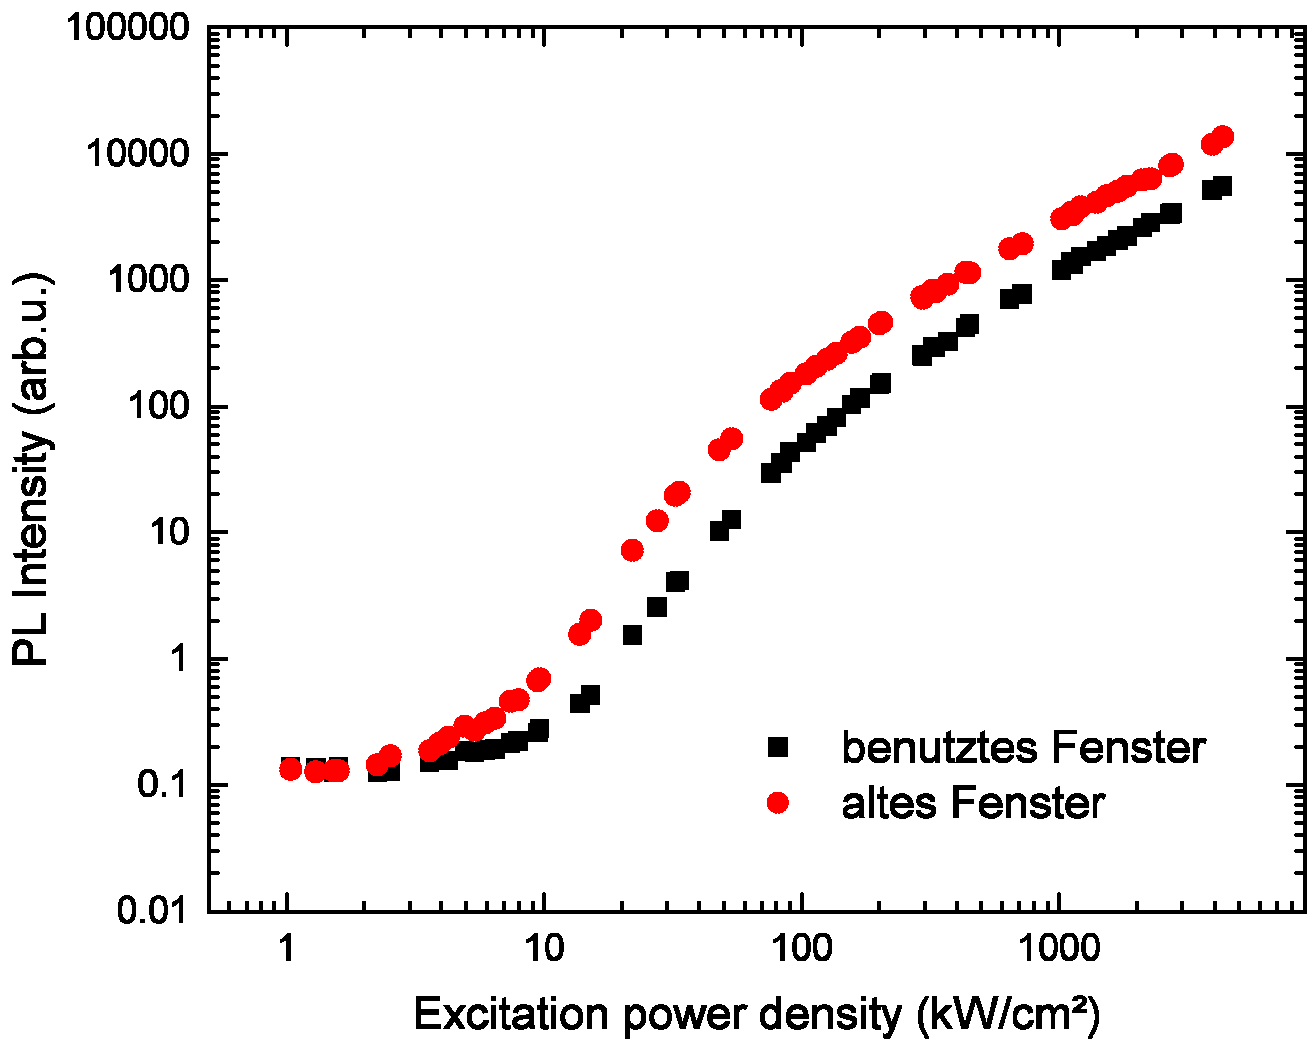
\includegraphics[width=0.9\linewidth]{Bilder/uvsilicavergleich.pdf}
    \caption{PL Intensität in Abhängigkeit der Anregungsleistungsdichte mit den benutzten und unbenutzten Fenstern}
    \label{fig:sub1}
  \end{subfigure}%
  {\LARGE$\xrightarrow{\cdot 0,44}$}
  \begin{subfigure}{0.40\textwidth}
    \centering
    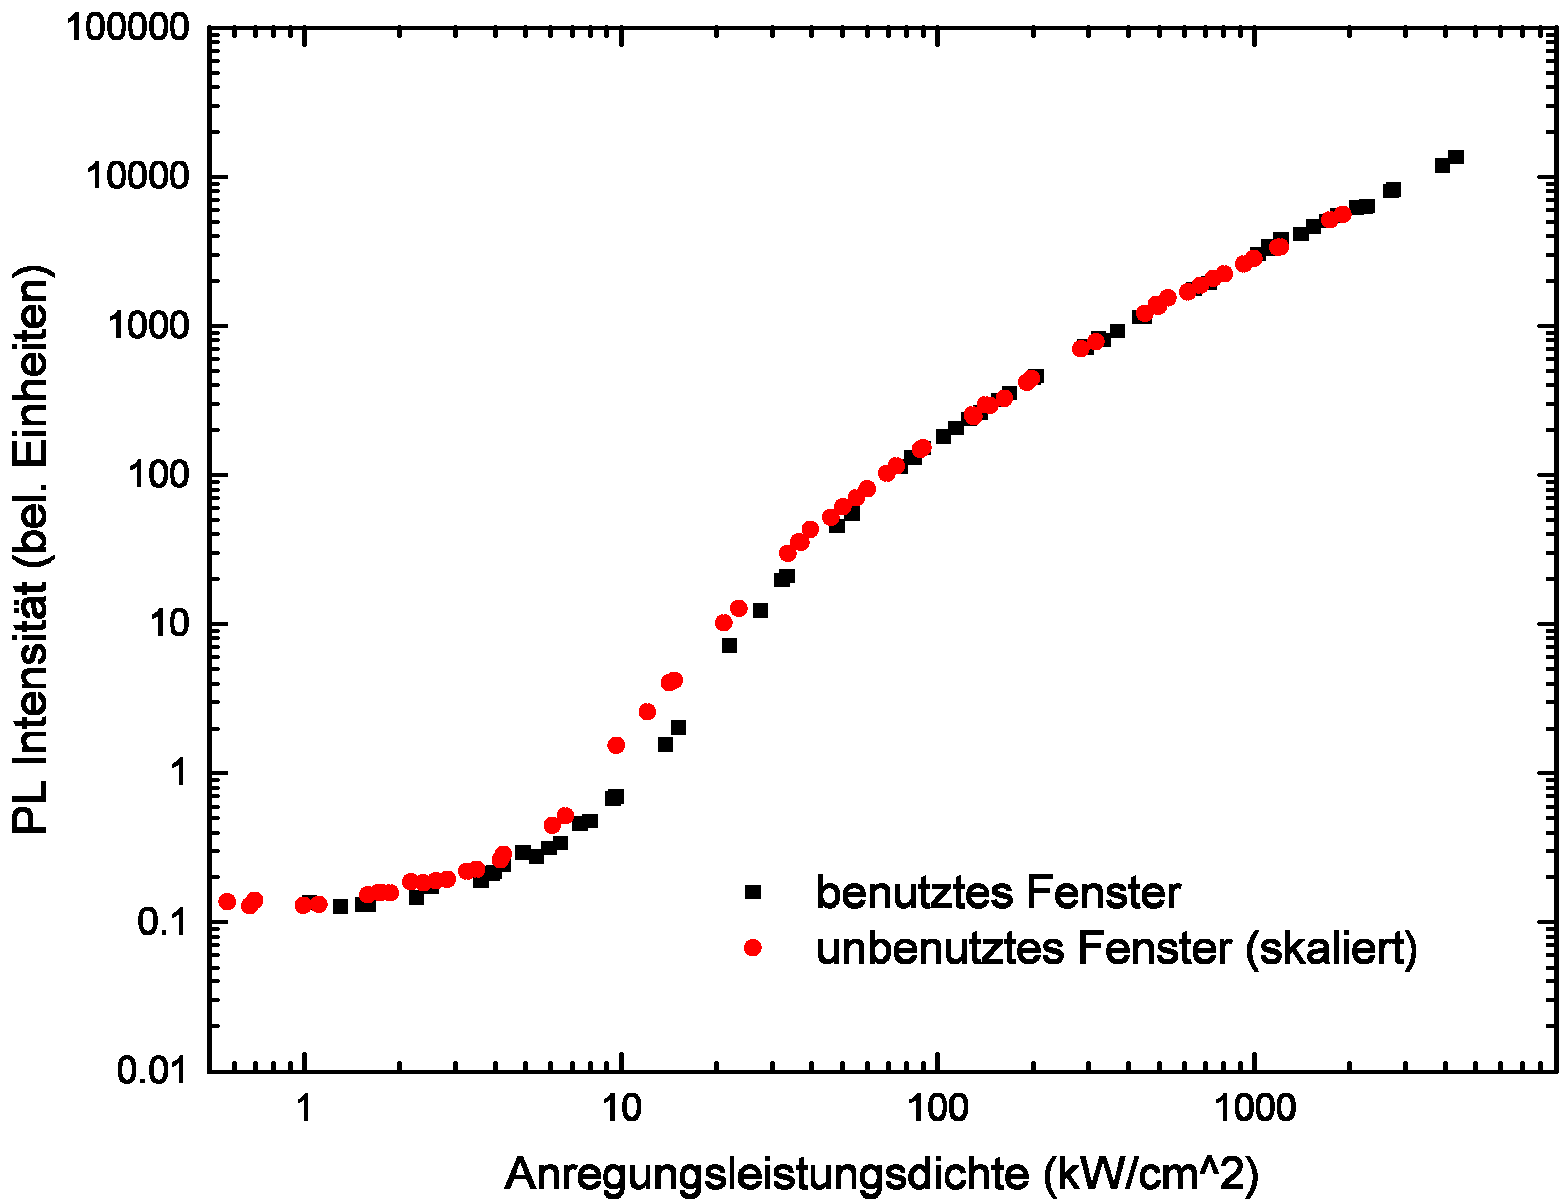
\includegraphics[width=0.9\linewidth]{Bilder/uvsilicaVergleichSkaliert.pdf}
    \caption{Die Anregungsleistungsdichte des unbenutzten Fensters mit den rechnerisch bestimmten 0,44 skaliert}
    \label{fig:sub2}
  \end{subfigure}
  \caption{}
  \label{fig:vergleichSkaliert}
\end{figure}
%
Um den Transmissionsgrad des benutzten Fensters zu bestimmen, wurde die Transmission durch das benutzte Fenster und dem parallel liegenden unbenutzten Fenster gemessen. Mit dem Wissen, dass der Transmissionsgrad durch das unbenutzte Fensters bei 59 Prozent ($T_{unb} = 0,59$), kann die Transmission durch das benutzte Fenster auf 26 Prozent ($T_{ben} = 0,26$) runtergerechnet werden. 
Davon ausgehend, dass die Transmission bei höheren Wellenlängen (Emission) gleich und bei beiden Fenstern ähnlich ist,
%
\begin{equation}
  F_{skal} = \frac{ T_{ben} }{ T_{unb} } = 0,44\label{eq11}
\end{equation}
%
kann der Skalierungsfaktor mit für die Anregungsleistungsdichte auf 0,44 bestimmt werden. Was bedeutet, dass durch Degradation die Transmission auf 44 Prozent der ursprünglichen Transmission gesunken ist.
Dies bestätigt sich auch durch die Gegenüberstellung in Abb. ~\ref{fig:vergleichSkaliert}. Dies bedeutet, dass durch die zeitliche Degradation die Transmission auf 44 Prozent der ursprünglichen gesunken ist.
Im Umkehrschkuss bedeutet dies, dass von der Anregungsleistungsdichte durch die geringe Transmission der Fenster und Reflektion im und außerhalb des Kryostaten nur ca. 26 Prozent bei der Probe ankommen. 
	%\section{Aufbau: Erweiterung der Filterkombinationen}
\thispagestyle{fancy}

Im Zuge dieser Arbeit wurden für eine Erhöhung der Messpunkte und Verringerung von Rauschen bei der leistungsdichteabhängigen Messung der IQE die Anzahl der Filterkombination erhöht. Dafür wurden die alten zwei Filterräder durch drei neue ersetzt. 
%
\begin{figure}[ht!]
    \centering
    \begin{minipage}[t]{1\linewidth}
        \centering
        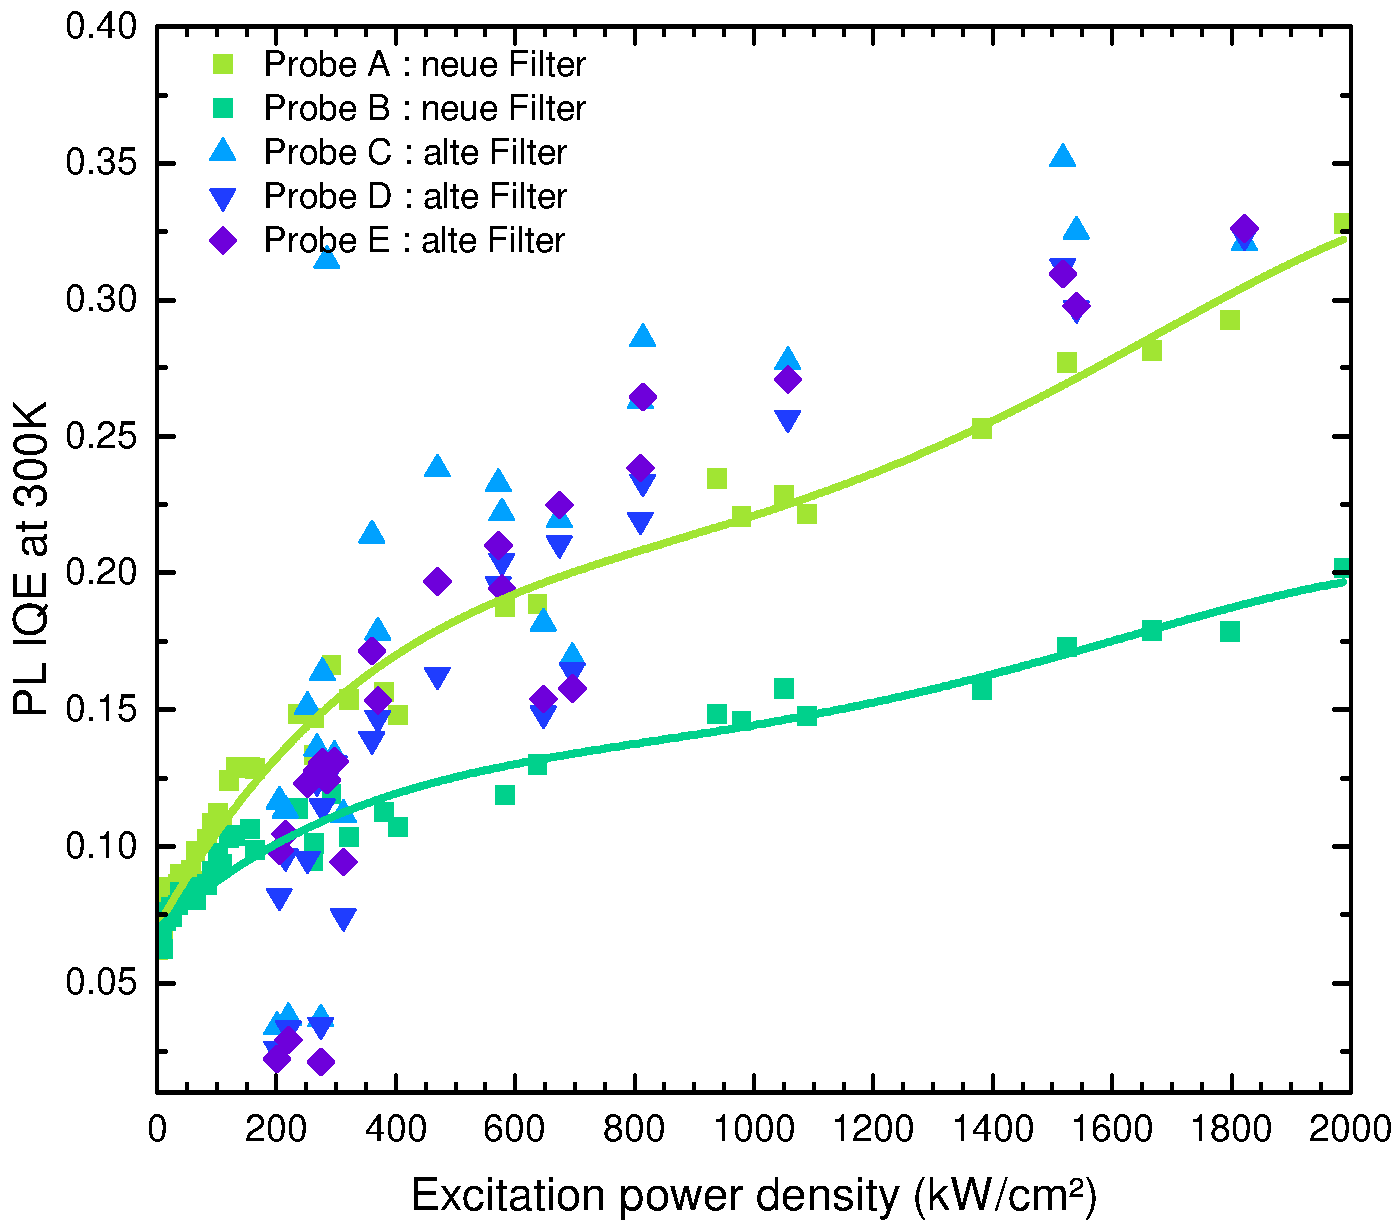
\includegraphics[width = 0.49\linewidth]{Bilder/AuswertungNovemeberKorr1VergleichFilter.pdf}
        \caption{Vergleich der Messung von insgesamt 5 ähnlichen Proben. 3 Proben (blau) wurden mit dem alten Setup gemessen. 2 Proben (grün, durchgezogene Linie) wurden mit dem neuen Setup gemessen. Die Präzision in tieferen Anregungsleistungsdichtenbereichen ist für das neue Setup deutlich erhöht. Das Rauschen fällt ebenfalls deutlich geringer aus. }
        \label{fig:vergleichFilter}
    \end{minipage}
\end{figure}
%
\newpage
Durch die erhöhte Anzahl möglicher Filterkombinationen ist es möglich, statt nur 27 verschiedene Messpunkte 61 zu nehmen. Speziell der Bereich der geringen Anregungsleistungsdichten kann so besser aufgelöst werden und das Rauschen wurde im Allgemeinen stark verringert \ref{fig:vergleichFilter}. 
%

	
\chapter{Einfluss der Auger-Rekombination auf die IQE}
\label{chap:auger}
\thispagestyle{fancy}
Das zum Zeitpunkt des Beginns dieser Arbeit verwendete Modell zur Bestimmung der PL-IQE ging davon aus, dass bei Tieftemperatur keine Auger-Rekombination (Gleichung \ref{eq:standardiqe}) vorkommt, aber wie in Abb. \ref{fig:auger5k} deutlich zu erkennen, nimmt der Verlauf der PL-Intensität in doppeltlogarithmischer Darstellung gegenüber der Anregungsleistungsdichte (die direkt proportional zur Ladungsträgerdichte ist), im Bereich höherer Anregungsleistungen (entsprechend höheren Ladungsträgerdichten) deutlich ab und weist keinen linearen Verlauf mehr auf, den er aber durch eine allein quadratische Abhängigkeit (in doppeltlogarithmischer Darstellung linear) haben sollte. 
\newline
\begin{figure}[ht]
    \centering
    \begin{minipage}[t]{0.49\linewidth}
        \centering
        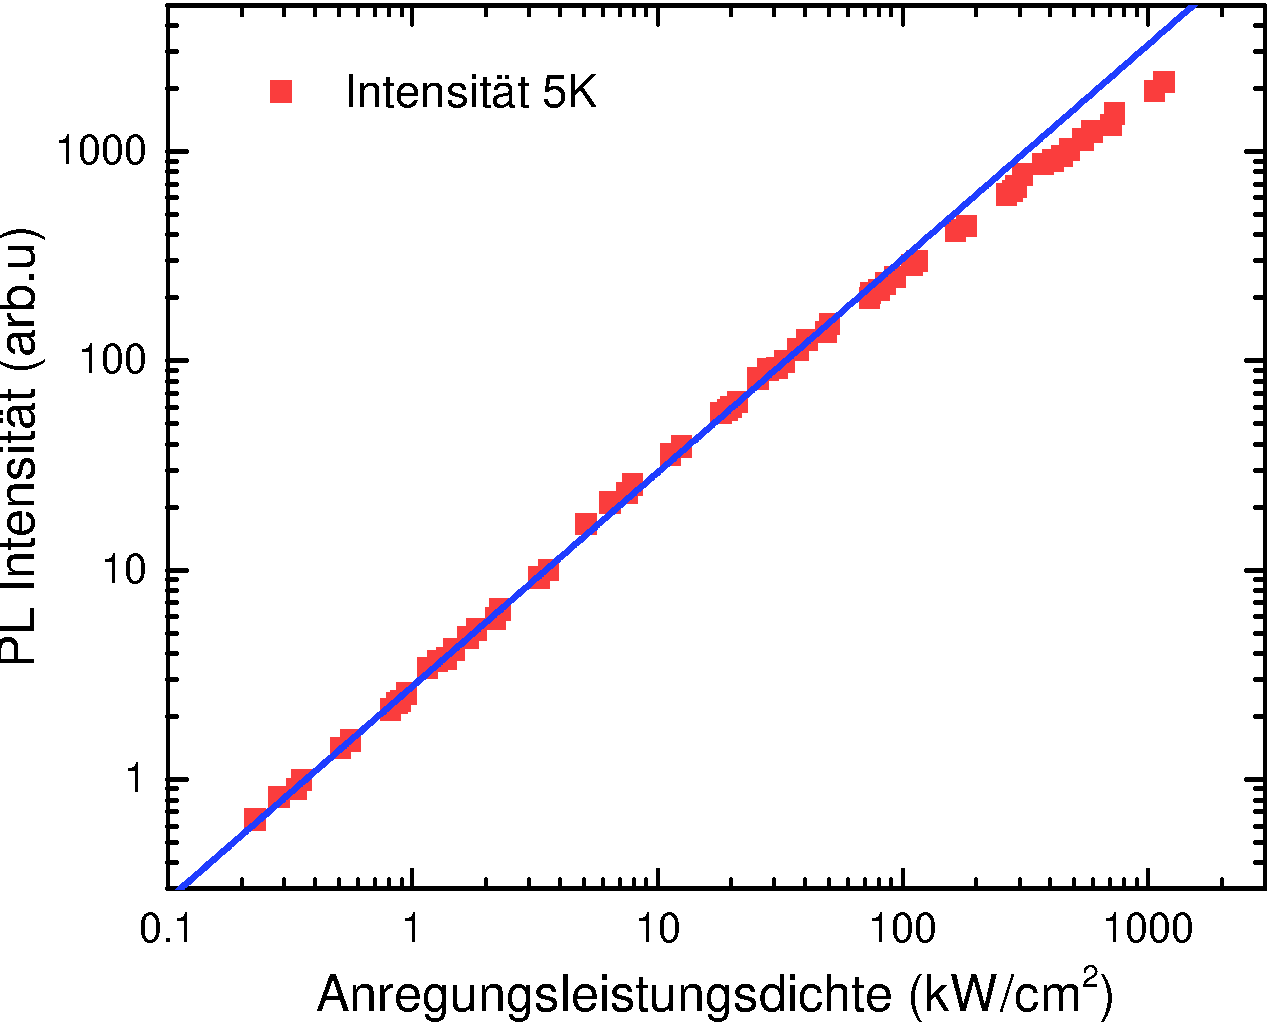
\includegraphics[width=\linewidth]{Bilder/AugerBei5K.pdf}
        \caption{Die Grafik zeigt die integrierte Intensität bei Tieftemperatur ($5 K$) in Abhängigkeit der Anregungsleistungdichte. In doppeltlogarithmischer Darstellung müsste die integrierte Intensität wegen $R = B \cdot n^2$ linear steigen (schwarze Linie).}
        \label{fig:auger5k}
    \end{minipage}% <- sonst wird hier ein Leerzeichen eingefügt
    \hfill
    \begin{minipage}[t]{0.49\linewidth}
        \centering
        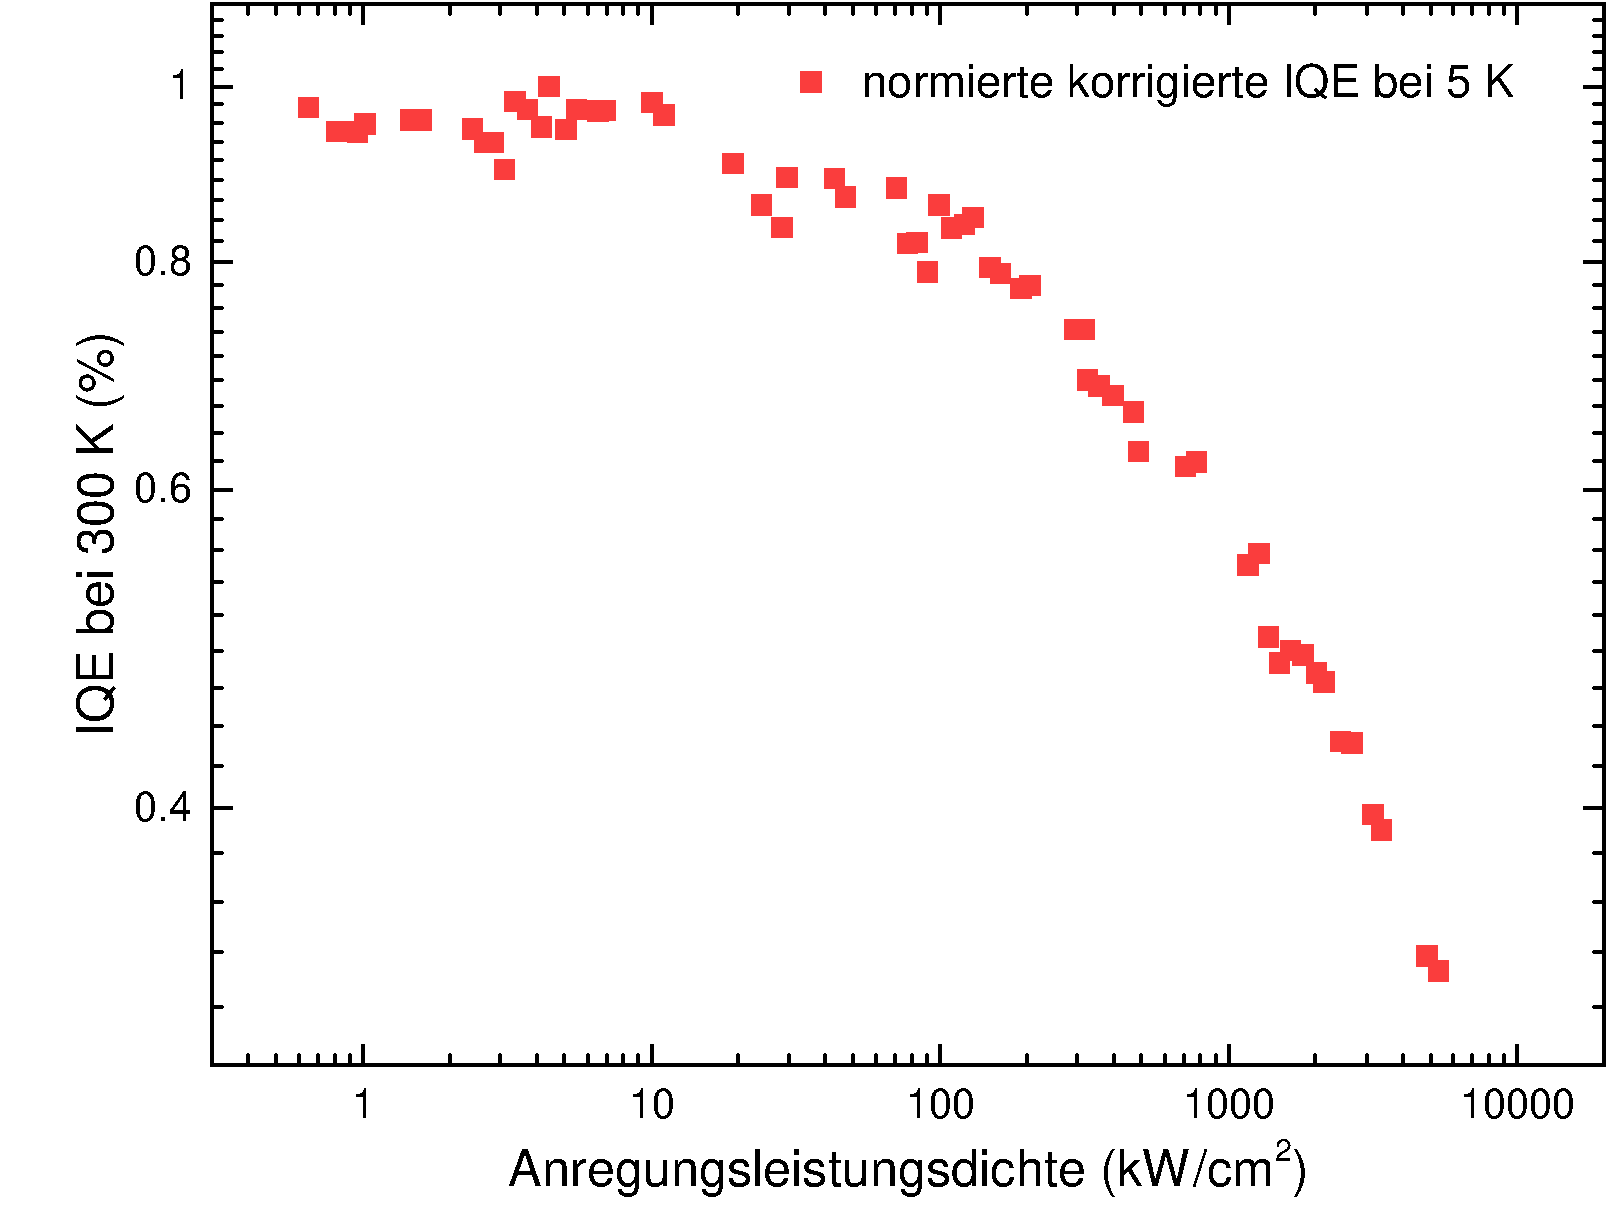
\includegraphics[width=\linewidth]{Bilder/NormierteKorrgierteIQE5K.pdf}
        \caption{Die Grafik zeigt die normierte korrigierte IQE bei 5K nach Gleichung \ref{eq:iqetrue5k}}
        \label{fig:trueiqe}
    \end{minipage}
\end{figure}
\vspace{0.1cm}
\noindent
\newline
Dies zeigt, dass die IQE bei Tieftemperatur nicht, wie bisher angenommen, immer bei 100 Prozent liegt, sondern auch bei Tieftemperatur anregungsleistungsdichteabhängig ist. Das dieser Verlustmechanismus ähnlich wie bei InGaN/GaN auf Auger-Rekombination basiert wurde von Nippert et al. bestätigt \cite{doi:10.1063/1.4965298}. 
Um dies zu berücksichtigen, wird nun die IQE bei 5K definiert als:
\begin{equation}
    IQE_{corr}(T = 5K, P_{exc}) = \frac{ \frac{I_{pl}(T,P_{exc}) }{P_{exc} } } { I_{norm}}
    \label{eq:iqetrue5k}
\end{equation}
mit dem Maximum der Verhältnisse von integrierter PL-Intensität zu Anregungsleistungdichte als  Normierungsfaktor über alle $n$ Anregungsleistungdichten
\begin{equation}
    I_{norm} = \lvert \lvert \sum_{i=1}^{n} \frac{I_{pl}(T,P_{exc,i})}{P_{exc,i}} \lvert \lvert_{max}
    \label{eq:iplnorm}
\end{equation}
\noindent
\begin{figure}[htb]
\centering
    \begin{minipage}[t]{0.49\linewidth}
        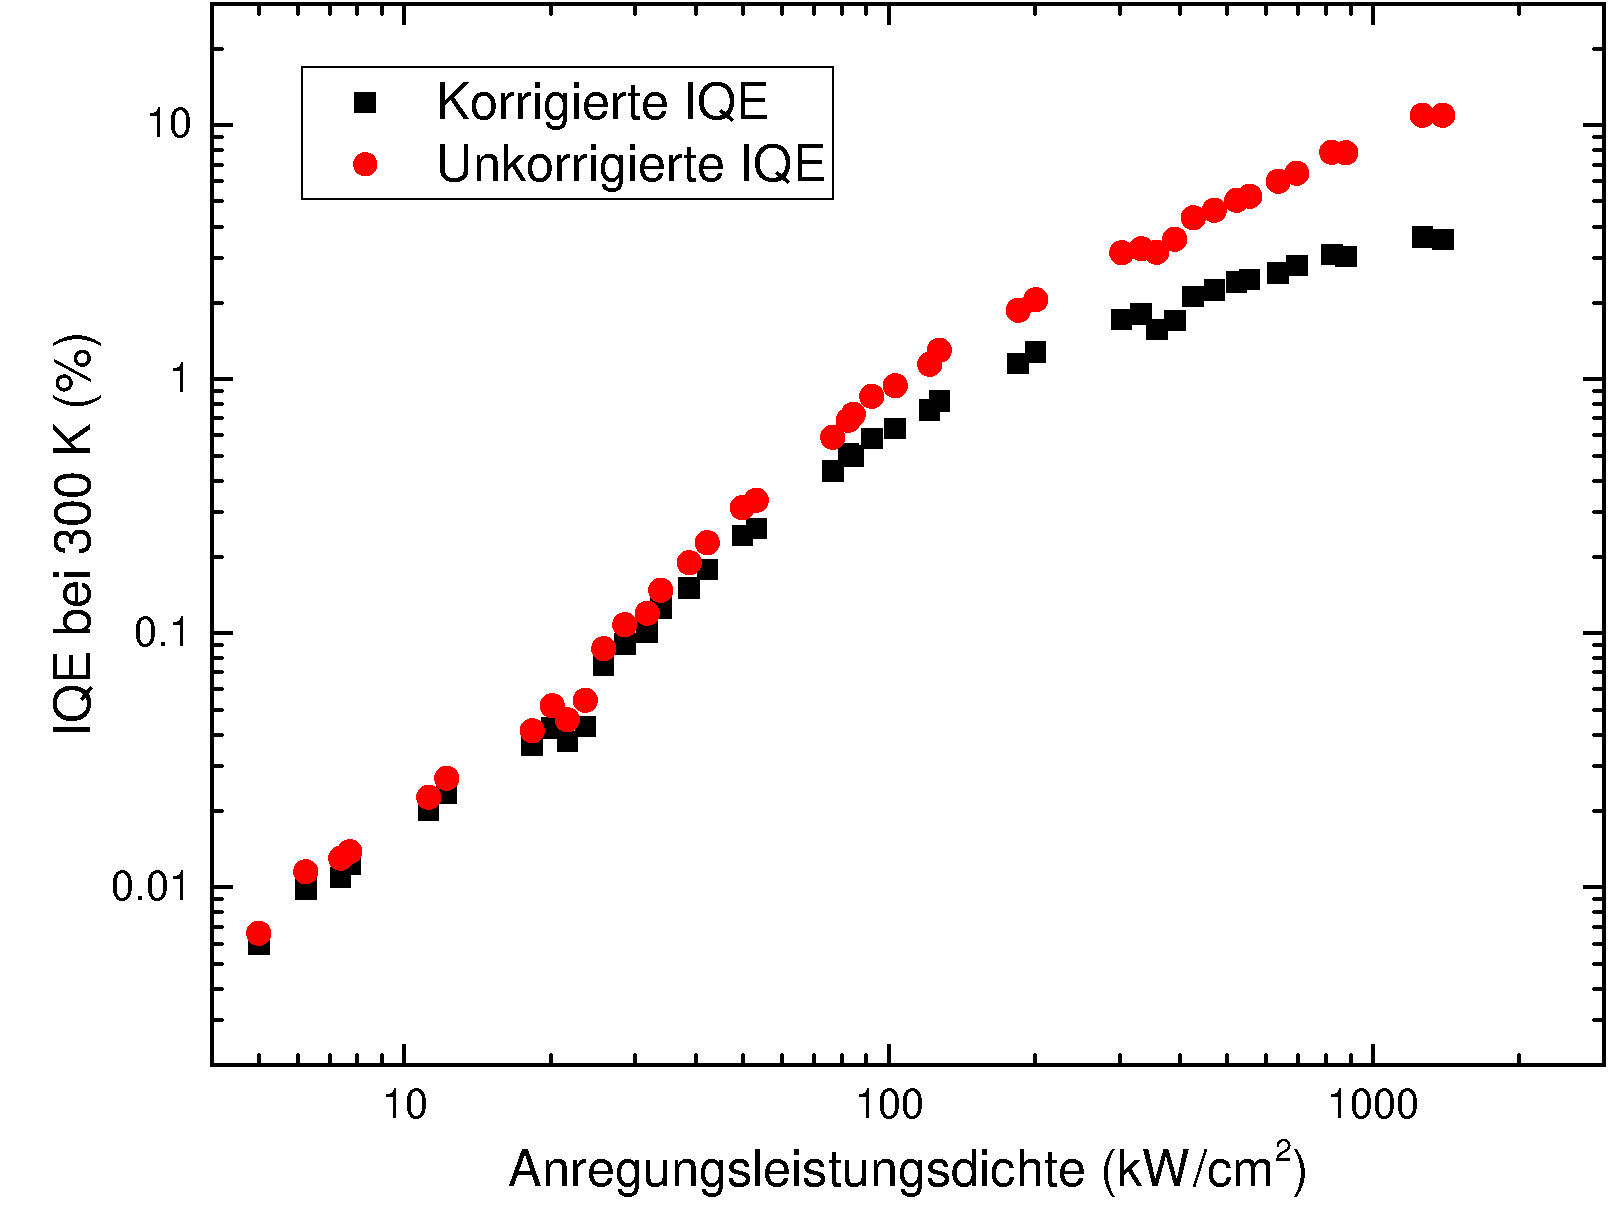
\includegraphics[width=\linewidth]{Bilder/korrigierteIQE300K.pdf}
        \caption{Vergleich von korrigierter und unkorrigierter IQE bei 300K nach Gleichung \ref{eq:iqetrue300k} }
        \label{fig:trueiqe300k}
    \end{minipage}
\end{figure}
\noindent
\newline
Wobei $I_{pl}(P_{exc})$ die von der Anregungsleistungsdichte $P_{exc}$ und Temperatur $T = 5K$ abhängige integrierte PL-Intensität ist. Die integrierte PL-Intensität wird durch die Anregungsleistungsdichte dividiert und auf das Maxmimum normiert, so dass die höchste IQE bei Tieftemperatur im Bereich der geringsten Anregungsleistungdichte mit der geringsten Auger-Rekombination liegen sollte. Um nun die IQE bei Raumtemperatur zu bestimmen, wird die nach dem alten Verfahren ermittelte IQE multipliziert mit den neu ermittelten Werten passend zur Anregungsleistungsdichte. 
\begin{equation}
    IQE_{corr}(T, A_{exc}) = \frac{IQE(T,A_{exc})}{IQE(5K,A_{exc})} \cdot IQE_{corr}(5K,A_{exc})
    \label{eq:iqetrue300k}
\end{equation}
Die IQE bei $5K$ dient hierbei also als Skalierungsfaktor, der den Einfluss der Auger-Rekombination bei einer bestimmten höher liegenden Temperatur (bspw. Raumtemperatur) korrigiert. Somit fällt im Vergleich insbesondere auf, dass die Skalierung bei den kleinsten Anregungsleistungsdichten den geringsten Einfluss hat und mit steigender Anregungsleistungsdichte kubisch steigt, so dass die nach dem alten Verfahren ermittelten IQE-Werte bei höheren Anregungsleistungsdichten deutlich nach unten korrigiert werden müssen. \newline
Auch wenn mit diesem Verfahren dem Einfluss der Auger-Rekombination mit berücksichtigt wird, so gibt es noch weitere Einflüsse die bei der IQE-Bestimmung beachtet werden müssen. Ein erhebliches Problem steckt in der nicht-resonanten Anregung mit dem ArF-Excimer Laser, denn das Laserlicht wird wegen der hohen Energie auch von allen Schichten und damit insbesondere in den Barrieren absorbiert. Die angeregten Ladungsträger müssen in den QW diffundieren und dort relaxieren, rekombinieren aber potentiell in den Barrieren, was im Spektrum als Barrieren Peak speziell bei Tieftemperatur zu sehen ist.
\newline
Daraus und aus Absorption resultierend scheitern oft AlGaN-Heterostrukturen die mit einem ArF Laser angeregt werden, eine Sättigung in der IQE zu erreichen \cite{doi:10.1063/1.4965298}. Ohne diese ist es schwer eine echte IQE anzugeben, da die in QWs gelangende Laserstrahlung, von nicht-resonanter Anregung ausgehend, von Materialparametern wie der Absorption und thermischen Diffusion abhängen und somit nicht klar ist, welche Anregungsleistungsdichte tatsächlich in die QWs gelangt. Weswegen ein Vergleich von Proben die sich in ihren Absorptionseigenschaften stark unterscheiden, schwer zu vergleichen sind, wenn die maximale IQE nicht bestimmt werden kann \cite{doi:10.1063/1.5044383}. 


	
	%\section{Einfluss der Siliziumdotierung auf die IQE}
\thispagestyle{fancy}
%
Das ABC-Modell stellt aber nur eine Vereinfachung dar und berücksichtigt nicht alle vorkommenden Effekte wie beispielsweise Lokalisierung, Screening durch Ladungsträger und Dotierung. 
Der Effekt der Dotierung spielt dabei eine besonders wichtige Rolle, da eine Silizumdotierung üblich in UV-Leds ist und einen großen Einfluss hat.
Nach \cite{schub} kann gezeigt werden, dass die Ratengleichungen, mit der Annahme einer Dotierung für die 
die Radiative Rekombination sich ändert und soll nun hergeleitet werden:
\\newline
Jeder dotierte oder undotiere Halbleiter hat zwei Arten von Ladungsträgern, Elektronen und Löcher.
Im Gleichgewicht, bedeutet ohne externe Anregung durch Absorption von Licht oder Injektion von Elektronen, ist das Produkt von Elektronen- und Lochkonzentration eine konstante Größe.
\begin{equation}
    n_0 \cdot p_0 = n_i^2
    \label{eq:constant}
\end{equation}
Hierbei sind $n_0$ und $p_0$ die Elektron- und Lochkonzentration unter Gleichgewichtsbedingung und $n_{i}$ damit die intrinsische Ladungsträgerkonzentration.
Werden zusätzlich die durch Anregung erzeugten Ladungsträger betrachtet, so ist die Gesamtladungsträgerkonzentration gegeben als Summe der Anregungs- und Gleichgewichtsladungsträger. 
\begin{equation}
    n_{ges} = n_0 + n \medspace \text{und} \medspace  p_{ges} = p_0 +  n 
\end{equation}
Hierbei sind $ n$ und $p$ die Anregungsladungsträger. 
Die Anzahl der stattfindenden Rekombination zwischen Elektronen und Löchern sind direkt proportional zur Elektronen-und Ladungsträgerkonzentration, so gilt, $R \propto n \cdot p $. Mit einer Proportionalitätkonstante, wird Rekombinationrate pro Zeit und Volumen definiert als
\begin{equation}
    R = - \frac{dn_{ges}}{dt} = - \frac{dp_{ges}}{dt} = B \cdot n_{ges} \cdot p_{ges}
\end{equation}
Weil Elektronen und Löcher bei Anregung paarweise erzeugt werden und verschwinden (durch Rekombination), gilt
\begin{equation}
    \label{eq:gleich}
    n(t) =  p(t)
\end{equation}
Die radiative Rekombinationrate wird dann mit $p_{0} = 0$ und Gleichung [\ref{eq:gleich}] zu
\begin{align}
\begin{split}
    R_{rad} &= B \cdot (n_0 + n)  \cdot (p_0 + p) ,
    \\
    R_{rad} &= B \cdot (n_0 + n) \cdot (n) ,
    \\
    R_{rad} &= B \cdot n^2 \cdot n \cdot n_0
\end{split}
\end{align}
Dabei beschreibt $n_{0}$ die Ladungsträgerkonzentration durch die Silizumdotierung. 
Somit wird die IQE zu:
\begin{equation}
    IQE = \frac{B \cdot n^2 + B \cdot n \cdot n_{0}}{A \cdot n + B \cdot n^2  + B \cdot n \cdot n_{0}+ C \cdot n^3} 
    \label{eq:dopediqe}
\end{equation}
Und hat einen enormen Einfluss auf die Ordinate, wie in Abb. [\ref{fig:abha1}] zu sehen ist.
%


	\thispagestyle{fancy}

\chapter{Untersuchung der optischen Polarisation an AlGaN MQWs mit Photolumineszenzspektroskopie}
\label{chap:pol}
\section{Einleitung}
Um die Polarisation und den Kreuzungspunkt der Simulationen von Christoph Reich experimentell zu \"uberpr\"ufen, wurden die Polarisation von zwei Probenserien mit Hilfe von Photolumineszenz-Spektroskopie untersucht. Die untersuchten Probenserien unterteilen sich in eine QW-Dicken-Variation (Serie A) und einer Serie mit Variation des Al-Gehalts (Serie B) in den QWs. 
Die Proben wurde alle bei Raumtemperatur (300K) untersucht und die Emission wurde aus der Kante der Probe gemessen um eine Absorption und Einfluss an der obersten Barriere zu vermeiden. Weil es m\"oglicherweise Auswirkungen des ELO auf die Polarisation gibt, wurde der Einfluss des ELO mit untersucht. 

\section{Variation des Al-Gehalts in den QWs}

Die Untersuchung der Al-Variations Serie, dient dem Zweck, anhand eines variierenden Al-Gehalts in den QWs und einem festen Al-Gehalt in der Barriere den \"Ubergang von TE zu TM (siehe Abb. [\ref{fig:simuchr}] in Kapitel \ref{chap:polgrund}) bei fester QW-Dicke experimentell zu \"uberpr\"ufen. Dazu wurden vier Proben auf ELO-AlN gewachsen, mit einer darauf folgenden AlN(100\%) Buffer-Schicht. Auf die Buffer-Schicht folgt zuletzt die aktiven Zone, mit einem zwischen der ersten und letzten undotierten AlN-Barriere eingebetteten dreifach $Al_{x}Ga_{1-x}N$ QWs mit einer Dicke von $1,5nm$ und dazwischen AlN-Barrieren einer Dicke von $5nm$. Der Aluminium-Gehalt der QWs wurde variiert mit x= 60 \%, 68 \%, 73 \%, 81 \%. 
Der Einfluss des unterschiedlichen Al-Gehalts auf die Emissionsenergie ist in Abb. [\ref{fig:alvariationSpektrum}] zu erkennen. Die kleinste Wellenl\"ange hat Probe A:4 mit einem Al-Gehalt von $81\%$, die theoretisch ausreicht um im Vergleich mit den anderen Proben zumindest einen Abfall des Polarisationgrades der TE-Polarisation zu erkennen.
%
\begin{figure}[htb]
  \centering
  \begin{minipage}[t]{0.49\textwidth}
    \centering
    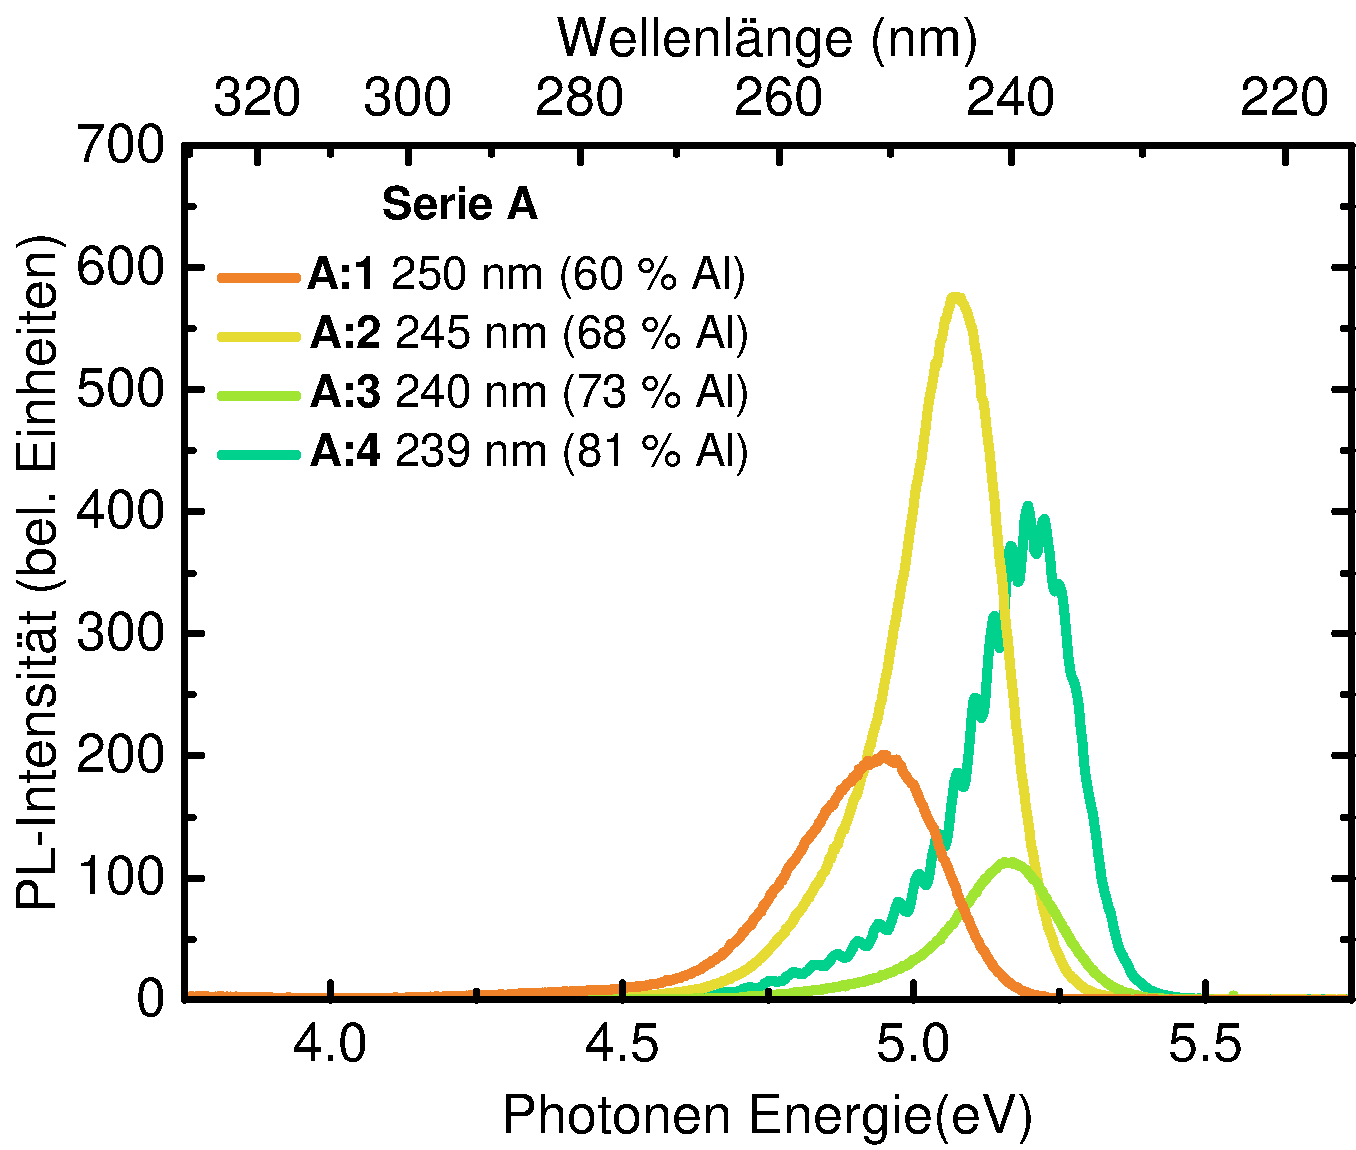
\includegraphics[width=\textwidth]{Bilder/spektrenAlvariation.pdf}
    \caption{PL-Spektren der Serie A. Die Emission verschiebt sich mit steigendem Al-Gehalt in den QWs hin zu kleineren Wellenl\"angen durch die steigende Bandl\"uckenenergie. }
    \label{fig:alvariationSpektrum}
  \end{minipage}
	\hfill
  \begin{minipage}[t]{0.49\textwidth}
    \centering
    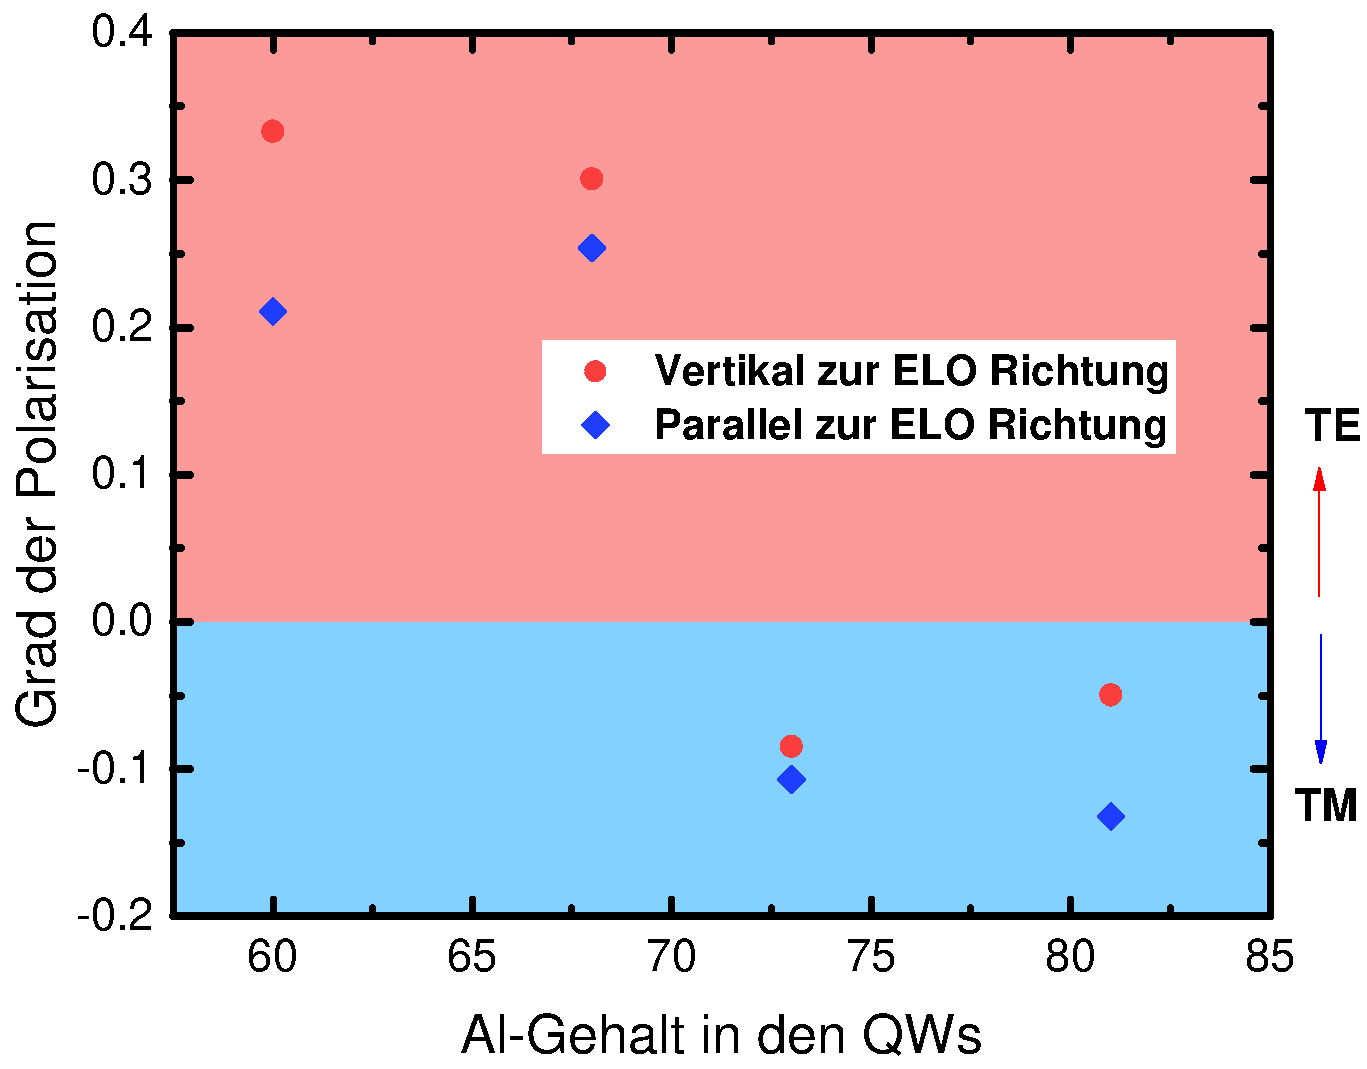
\includegraphics[width=\linewidth]{Bilder/polarisationAlvariation.pdf}
    \caption{Ergebnisse der Polarisationsmessungen an Serie A mit den Polarisationsgraden abh\"angig vom Al-Gehalt des QW und zus\"atzlich mit den Messwerten in Abh\"angigkeit der ELO-Richtung. }
    \label{fig:alvariationPolarisation}
  \end{minipage}
\end{figure}
%
Dazu wurden Proben vertikal und horizontal zur ELO-Richtung positioniert und gemessen. Abbildung [\ref{fig:alvariationPolarisation}] zeigt die Ergebnisse der Polarisationsmessungen. So zeigen die Proben A:1 und A:2 mit einem Al-Gehalt von $60\%$ und $68\%$ TE-Polarisation. Der Grad der Polarisation ist zus\"atzlich noch abh\"angig von der Positionierung der ELO-Streifen. So haben die Proben A:1 und A:2 vertikal zur ELO-Richtung Polarisationsgrade von $\rho = 0,33$ und $\rho = 0,30$ und parallel zur ELO-Richtung deutlich geringe Polarisationsgrade mit $\rho = 0,22$ und $\rho = 0,25$. Die Proben A:3 und A:4 mit $73\%$ und $81\%$ Al-Gehalt weisen TM-Polarisation auf mit Polarisationsgraden von $\rho = -0,09$ und $\rho = -0,05$ vertikal zur ELO-Richtung und $\rho = -0,11$ und $\rho = -0,14$ parallel zur ELO-Richtung. Es zeigt sich demzufolge, dass die Polarisation sich mit steigendem Al-Gehalt von TE- hin zu TM-Polarisation \"andert durch die Neuordnung der Valenzb\"ander. Der Wechsel findet bei einer Wellenl\"ange von ca. $240nm$ statt und ist in guter \"Ubereinstimmung mit den Simulation (siehe Abb. [\ref{fig:simuchr}]). \"Uberdies ist eine Abh\"angigkeit der Ausrichtung der ELO-Streifen zu beobachten. M\"ogliche Erkl\"arungen w\"aren, dass es durch Brechungsindexwechsel vom Freiraum des ELO zum Kristall, es zu Reflektion des emittierten Lichtes und damit zu Interferenzerscheinungen kommt oder das ELO beeinflusst die Verzerrung im Kristall so, dass die f\"ur die Simulation angenommene biaxiale Verzerrung nicht mehr zutrifft. 

\section{Variation der QW-Dicke}

Die Untersuchung der QW-Dicken Variations Serie, dient dem Zweck, anhand der variierenden QW-Dicke bei einem festen Al-Gehalt in QW und Barriere den \"Ubergang von TE zu TM (siehe Abb. [\ref{fig:simu1chr}] in Kapitel \ref{chap:polgrund}) experimentell zu \"uberpr\"ufen. Dazu wurden vier Proben auf ELO-AlN gewachsen, mit einer darauf folgenden AlN(100\%) Buffer-Schicht. Auf die Buffer-Schicht folgt zuletzt die aktiven Zone, mit einem zwischen der ersten und letzten undotierten AlN-Barriere eingebetteten dreifach $Al_{0.6}Ga_{0.4}N$ QWs und dazwischen $Al_{0.81}Ga_{0.19}N$-Barrieren einer Dicke von $5nm$. 
Der Einfluss des unterschiedlichen QW-Dicke auf die Emissionsenergie ist in Abb. [\ref{fig:qwvariationSpektrum}] zu erkennen. Mit steigender QW-Dicke sinkt die Emissionsenergie und steigt die Wellenl\"ange aufgrund des QCSE und Confinements. Die Emission der Barriere ist mit steigender Dicke besser erkennbar. 
%
\begin{figure}[htb]
  \centering
  \begin{minipage}[t]{0.49\textwidth}
    \centering
    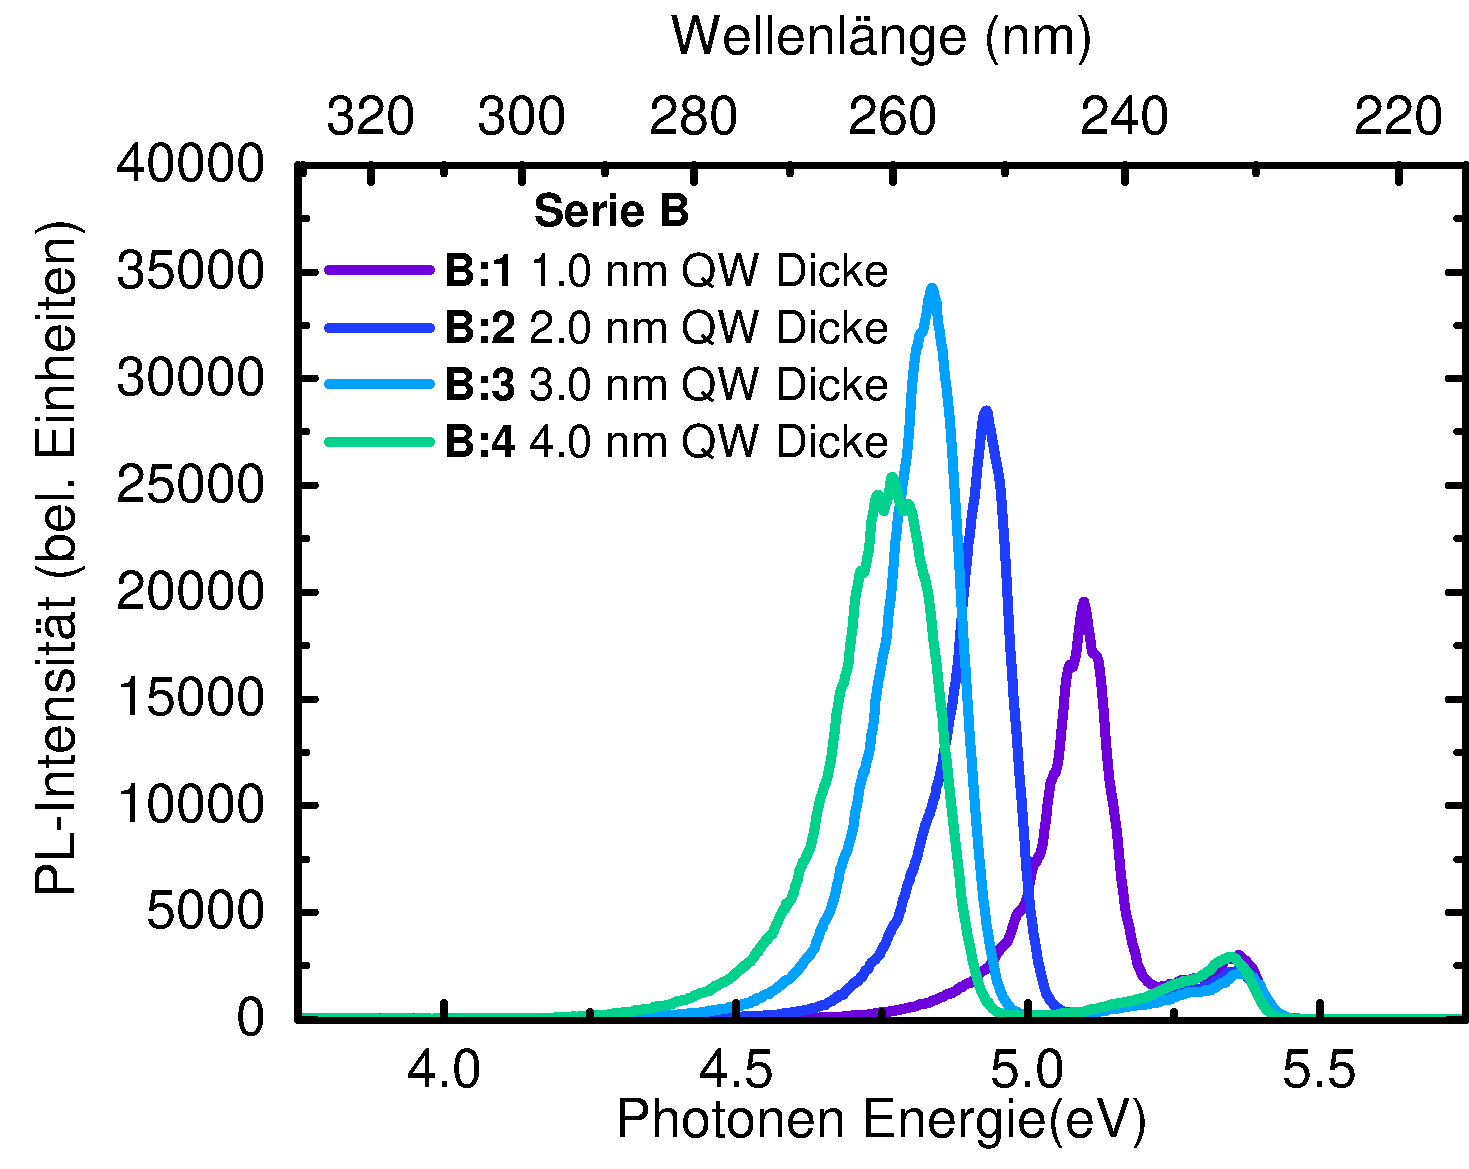
\includegraphics[width=\textwidth]{Bilder/spektrenQWvariation.pdf}
    \caption{PL-Spektren der Serie B. Die Emission verschiebt sich mit steigender QW-Dicke hin zu gr\"oßeren Wellenl\"angen durch den QCSE und Confinement.  }
    \label{fig:qwvariationSpektrum}
  \end{minipage}
	\hfill
  \begin{minipage}[t]{0.49\textwidth}
    \centering
    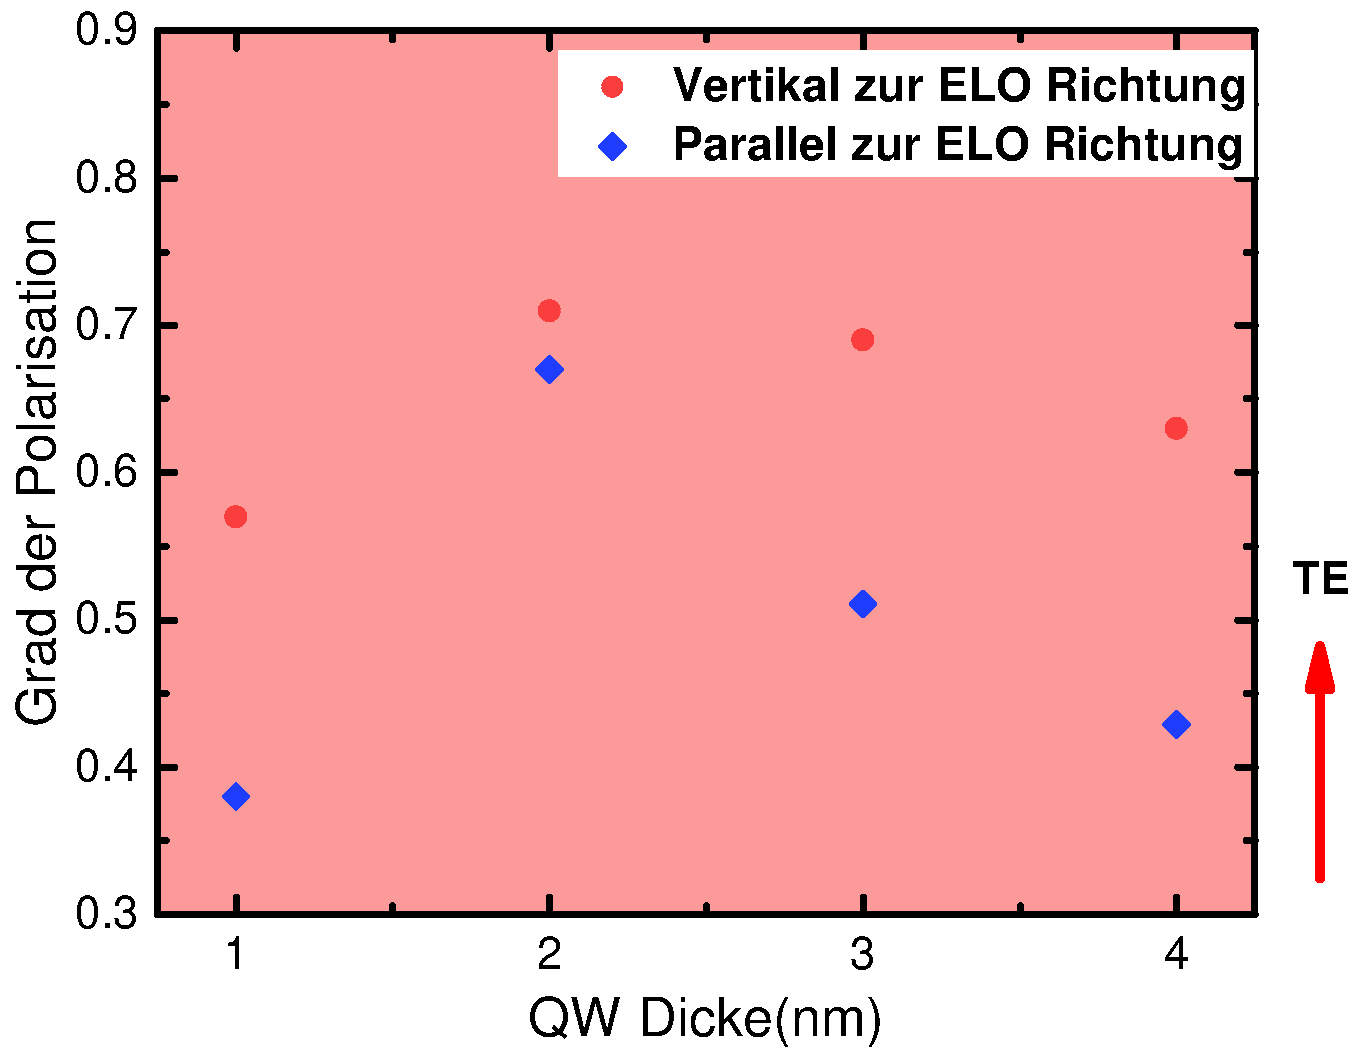
\includegraphics[width=\linewidth]{Bilder/polarisationDickenvariation.pdf}
    \caption{PL-Spektren der Serie B. Die Emission verschiebt sich mit steigendem Al-Gehalt in den QWs hin zu kleineren Wellenl\"angen durch die steigende Bandl\"uckenenergie. }
    \label{fig:qwvariationPolarisation}
  \end{minipage}
\end{figure}
%
die Ergebnisse der Polarisationsmessung zeigen eine eindeutig dominante TE-Polarisation die auch abh\"angig von der ELO-Richtung ist. Die Probe B:2 zeigt die h\"ochste TM-Polarisation mit einem Polarisationgrad von $\rho=+0,72$ vertikal zur ELO-Richtung. 



	%\chapter{Ergebnisse}
\thispagestyle{fancy}
\section{Untersuchung optisch gepumpter Laserstrukturen auf unterschiedlichen Templates}


Dieses Kapitel widmet sich der Untersuchung der beiden Probenreihen TS4045 und TS4048 von optisch gepumpten Laserstrukturen die aus Rezepten aus zwei unterschiedlichen Serien stammen. Die beiden Serien unterscheiden sich im wesentlichen dadurch, dass sie mit(TS4048) und ohne Übergitter(TS4045) gewachsen wurden. Jede Reihe für sich weist  zusätzlich noch Unterschiede den Proben selbst auf, so sind zwei Proben der Reihe TS4045 auf AlN-Bulk zweier unterschiedlicher Hersteller (HexaTech, IKZ) gewachsen und alle  anderen Proben auf ELO AlN/Sapphire mit jeweils 3 unterschiedlichen "offcut"-Winkeln. Tabellerisch sieht die  Zusammenstellung wie folgt aus: 

\vspace{1cm}


\setlength{\arrayrulewidth}{0.5mm}
\setlength{\tabcolsep}{0.5pt}
\renewcommand{\arraystretch}{1.5}
 

\begin{tabular}{ |c|c|c|c|c|c|   }
\hline
\multicolumn{3}{|c|}{TS4045} & \multicolumn{3}{c|}{TS4048}  \\
\hline
Endung & offcut& Template & Endung & offcut& Template \\
\hline
-2V* & 0.1$^\circ$m & ELO & -2V* & 0.1$^\circ$m & ELO \\
-2H & 0.1$^\circ$m & ELO & -2H & 0.1$^\circ$m & ELO \\
-2Z & 0.2$^\circ$m & ELO & -1 & 0.1$^\circ$m & ELO \\
-1 & 0.1$^\circ$m & Bulk(IKZ) & -2V* & 0.1$^\circ$m & ELO \\
-3* & 0.1$^\circ$m & Bulk(Hexatech) & -2V* & 0.1$^\circ$m & ELO \\
\hline



\end{tabular}



	

	\bibliography{Bibliographie}
\end{document}	


\begin{comment}
	\begin{figure}[b!]
    		
\includegraphics[width=0.2\textwidth]{Bilder/TU-Berlin-Logo.pdf}
    		\label{fig:tulogo}
    	\end{figure}	
\end{comment}	
